% =====================================================================
% Master's Thesis -- master document
% Wires the abstract plus five chapter files (ch0_abstract, ch1 .. ch5) into one
% FPT-template report-class PDF. Build from THIS directory:
%     latexmk -pdf main.tex
% (or: pdflatex main; bibtex main; pdflatex main; pdflatex main)
%
% Each ch*.tex is a body FRAGMENT (no preamble, no \begin/\end{document});
% top-level headings were promoted \section->\chapter, \subsection->\section,
% \subsubsection->\subsection at assembly. Cross-chapter references are real
% \ref{} into the shared label namespace this file creates.
% =====================================================================
\documentclass[a4paper,12pt]{report}

% --- Base packages (union of every fragment + the FPT template) ---
\usepackage[english]{babel}
\usepackage{indentfirst}  % indent the first paragraph after every heading too
\usepackage[utf8]{inputenc}
\usepackage[T1]{fontenc}
\usepackage{lmodern}
\usepackage{amsmath,amssymb,amsfonts}
\usepackage{bm}
\usepackage{booktabs}
\usepackage{float}
\usepackage{siunitx}
\usepackage{microtype}
\usepackage{graphicx}
\usepackage{multirow}
\usepackage{array}
\usepackage{url}
\usepackage[super]{nth}
\usepackage[margin=2.5cm]{geometry}
\usepackage{fancyhdr}

% --- Chapter 3 pipeline diagram ---
\usepackage{tikz}
\usetikzlibrary{arrows.meta,positioning,fit,backgrounds,calc,shapes.geometric}

% --- Custom siunitx units used in the timing tables/figures (Ch 3-4) ---
% (\frame is otherwise the LaTeX kernel box-frame command, not a unit.)
\DeclareSIUnit{\frame}{frame}
\DeclareSIUnit{\fps}{fps}

% --- Figures ---
% Committed copies live in figures/ (tracked, so the thesis builds from a plain
% clone on any machine). The gitignored output/ tree is kept as a fallback so a
% freshly regenerated figure is still picked up on the authoring machine.
% Paths are relative to this master in docs/writing/thesis/.
\graphicspath{{figures/}{../../../output/figures/}{../../../output/experiments/}}

% --- Header / footer (FPT template style) ---
\setlength{\headheight}{15pt}
\addtolength{\topmargin}{-3pt}
\pagestyle{fancy}
\fancyhf{}
\lhead{FPT School of Business \& Technology}
\cfoot{\thepage}
\renewcommand{\headrulewidth}{0.5pt}
\renewcommand{\footrulewidth}{0.5pt}

\begin{document}
\sloppy

% --- Title page (FPT template style) ---
\begin{titlepage}
  \begin{center}
    
\includegraphics[scale=0.3]{../report-template/Images/fpt.png}
  \end{center}

  \center
  \vspace{0.5in}
  \textbf{\large MASTER'S THESIS}
  \vspace{0.5in}

  \noindent\makebox[\linewidth]{\rule{\linewidth}{1.2pt}}
  \textbf{\large A Donor-Frame Coverage Metric for Evaluating
    Occluded-Vehicle Completion in Automotive LiDAR}
  \noindent\makebox[\linewidth]{\rule{\linewidth}{1.2pt}}

  \vspace{0.5in}

  \begin{minipage}{0.60\textwidth}
    \begin{flushleft}
      \textit{Student:} \\
      \vspace{0.1in}
      \begin{tabular}{|l|l|}
        \hline
        Ngo Vi Viet Anh & MSE13205 \\ \hline
      \end{tabular}
    \end{flushleft}
  \end{minipage}
  \begin{minipage}{0.35\textwidth}
    \begin{flushright}
      \textit{Advisor:} \\
      Dr. Doan Nhat Quang \\
    \end{flushright}
  \end{minipage}

  \vspace{2in}
  \textbf{\large Master's Thesis} \\
  \today
\end{titlepage}

% --- Front matter (roman page numbers) ---
\pagenumbering{roman}

% --- Keywords ---
\chapter*{Keywords}
\begin{itemize}\setlength{\itemsep}{2pt}
  \item Autonomous driving perception
  \item Automotive LiDAR
  \item Point cloud segmentation
  \item Vehicle detection
  \item Point cloud completion
  \item Occluded-vehicle completion
  \item Donor-frame coverage metric
  \item Reference-free evaluation
  \item Amodal bounding box
  \item SemanticKITTI
\end{itemize}
\clearpage

% Abstract removed per author request (2026-09-05); ch0_abstract.tex kept on disk, unwired.

% --- Acknowledgements and Declaration of Authorship ---
\chapter*{Acknowledgements and Declaration of Authorship}

\section*{Acknowledgements}
I would like to express my sincere gratitude to my thesis supervisor, \textbf{Dr. Doan Nhat Quang}, for his guidance, constructive feedback, and support throughout the development of this research. His academic advice and technical insights have been essential to the conceptualization and refinement of the proposed framework.

I am also grateful to the faculty and staff at the \textbf{FPT School of Business \& Technology (FSB)} for providing a structured academic environment and for the knowledge they have shared throughout the Master's programme. I also thank my colleagues and peers for their helpful discussions and feedback during the research process.

Finally, I wish to thank my family for their patience and support during the period of my graduate studies.

\section*{Declaration of Authorship}
I, \textbf{Ngo Vi Viet Anh}, student ID \textbf{MSE13205}, hereby declare that this thesis, entitled \textit{``A Donor-Frame Coverage Metric for Evaluating Occluded-Vehicle Completion in Automotive LiDAR''}, is the result of my own work carried out under the supervision of Dr. Doan Nhat Quang at the FPT School of Business \& Technology.

I solemnly declare that:
\begin{itemize}
    \item The research presented in this work, including the donor-frame coverage metric, the hybrid detection-and-completion pipeline, and the evaluation of occluded-vehicle completion, is my own original work unless otherwise referenced.
    \item All experimental results and quantitative evaluations reported in Chapter~\ref{ch:evaluation} are authentic and have been obtained through testing on the specified datasets. No data fabrication or manipulation has taken place.
    \item All sources of information utilized in this thesis have been cited in accordance with standard academic referencing practices.
    \item This thesis has not been submitted, in whole or in part, for any other degree or qualification at this or any other institution.
\end{itemize}

I take full responsibility for the content, accuracy, and academic integrity of this thesis.
\clearpage

\tableofcontents
\listoffigures
\listoftables
\clearpage

% --- Body (arabic page numbers) ---
\pagenumbering{arabic}

% Chapter 1 -- Introduction (\input by main.tex)
% Frames the problem, the modular approach, the two research questions, the
% contribution, the scope, and the thesis outline.
% Published literature uses BibTeX \cite{}.
%
% CONSISTENCY CONSTRAINTS (checked at draft time):
%   - Every claim here is a subset of the claims map (C1--C11).
%     Nothing is stated beyond the PARTIALLY-HOLDS scope of the held-out completion
%     result (C9). The single scientific contribution (the donor metric) matches
%     Chapter 2's Sec 2.5; the two diagnostic findings (recall root-cause /
%     synthetic-pretraining redundancy) are reported as findings, not contributions;
%     the pipeline, runtime characterisation, and amodal-GT builder are named as
%     ENGINEERING contributions, and tracking is explicitly not a contribution.
%
% Honesty-phrasing rules applied (personal_agenda P1):
%   - recall is stated against its car-only, >=10-surviving-points denominator
%   - the held-out completion result is PARTIALLY HOLDS, never unqualified
%   - negative results are named as findings, not buried
%   - the detection headline is a single-sequence (seq 08) result, stated as such
%
\chapter{Introduction}
\label{ch:introduction}

\section{Background and Rationale}
\label{sec:intro-background}

Autonomous driving depends on a perception system that can recover, several times a
second, the three-dimensional layout of the scene around the vehicle: where the other
road users are, how large they are, and which way they face. LiDAR is central to this
task. It measures range directly, returning an unordered cloud of over a hundred
thousand points per scan, largely invariant to lighting and carrying the metric depth
that motion planning needs. The benchmarks that opened the field were built around it:
the KITTI suite~\cite{geiger2012we} paired a scanning LiDAR with calibrated cameras,
and its point-wise successor SemanticKITTI~\cite{Behley_2019_ICCV} turned the same
sequences into the dense segmentation benchmark much of the field is now measured
against.

The dominant paradigm is to train a deep network end to end on annotated scans:
point-based segmentation networks~\cite{Qi_2017_CVPR,NIPS2017_d8bf84be,Hu_2020_CVPR},
projection- and voxel-based models~\cite{10.1109/ICRA.2018.8462926,milioto2019rangenet++,zhu2021cylindrical},
single-pass object detectors~\cite{lang2019pointpillars,yin2021centerpoint}, and
panoptic models~\cite{zhou2021panopticpolarnet,hong2021dsnet}. These define the state
of the art in accuracy, which is paid for in two costs. The first is supervision: the
results rest on dense, point-wise labels, and the annotation behind a benchmark like
SemanticKITTI --- a class on every one of billions of points --- is out of reach for
most groups and most new datasets. The second is opacity: an end-to-end network spreads
each decision across millions of weights, so when it misses a car there is no single
stage to inspect or repair.

This thesis takes the opposite starting point, asking how far a \emph{modular},
largely annotation-free pipeline can go: classical geometry for the parts geometry
solves well, and small learned models only where discrimination needs them --- an
approach to LiDAR vehicle detection that has drawn renewed interest~\cite{lim2025longrange}.
Clustering proposes candidate objects, a small binary \emph{car}/\emph{not-car}
classifier keeps the vehicles, and each detected car is completed by a PCN network;
every stage is separately inspectable, and the learned components are trained without
point-wise labels. Chapter~\ref{ch:pipeline} gives the full pipeline
(Figure~\ref{fig:pipeline}).

\section{Challenges in Real-Data Completion}
\label{sec:intro-challenges}

It is the second half of this pipeline that raises the problem the thesis is built
around. Completing a partially observed car --- recovering the far side the sensor
cannot reach --- is attractive for downstream box estimation, and networks such as
PCN~\cite{yuan2019pcnpointcompletionnetwork} are well studied on synthetic benchmarks.
On real LiDAR they cannot be evaluated: there is no clean ground-truth complete shape,
and the obvious substitute --- accumulating the same static car across many frames ---
is itself one-sided and, as this thesis shows, invalid as a reference, because the raw
partial input scores best against it. Before completion can be claimed to help,
it must be possible to measure at all. This is where the topic narrowed: an initial aim
of applying learned completion to real LiDAR ran into the fact that its quality could
not be measured validly at all, and that gap --- not the completion network itself ---
became the question the thesis is built around.

\section{Research Objectives}
\label{sec:intro-objectives}

The work is organised around two research questions about measuring and validating
completion on real LiDAR; the central contribution answers them, and two further
findings --- reported below in their own right --- record what the investigation
revealed about the detection front-end along the way.

\begin{enumerate}
  \item \textbf{A Valid Evaluation Method for Real-LiDAR Completion.}
    Establish how the quality of point-cloud completion can be evaluated on
    \emph{real} LiDAR, where no clean reference shape exists and an accumulated
    pseudo-ground-truth is itself one-sided --- a measurement question prior to any
    claim that completion helps (RQ1; answered in
    Section~\ref{sec:donor-validation}).
  \item \textbf{Evidence That Completion Recovers Unseen Surface.}
    Determine whether learned completion recovers genuinely \emph{unseen} surface,
    as opposed to redistributing the points it was already given; whether it
    improves downstream amodal bounding boxes on real LiDAR cars; and whether any
    such benefit survives on a held-out sequence under a pre-registered test (RQ2;
    answered in Section~\ref{sec:donor-validation}, with the held-out outcome
    reported exactly as it fell).
\end{enumerate}

\section{Research Contributions}
\label{sec:intro-contributions}

The thesis makes a single scientific contribution, methodological rather than
architectural, together with the engineering contributions that make it possible.

\begin{itemize}
  \item \textbf{A Validated Metric for Occluded-Vehicle Completion on Real LiDAR.}
    Chamfer distance against an accumulated pseudo-ground-truth is invalid on real
    cars, so the thesis defines a donor-frame occluded-side coverage metric: it
    scores how much of the surface seen only in other frames of the same
    static car a completion recovers, with a hallucination guard against surface
    invented outside the car's box, and validates it against a four-item gate.
    Applied to real sequence-08 cars, it shows that PCN recovers occluded surface
    several times above the symmetry-mirror baseline and improves amodal boxes on
    static, gate-passed cars, and that the benefit partially holds on a
    pre-registered held-out sequence (Section~\ref{sec:donor-validation}). The
    detection and completion stages are established building blocks, reimplemented
    and tuned here; the contribution is the measurement built on top of them.

  \item \textbf{A Modular, Near-Annotation-Free Detection-and-Completion Pipeline.}
    A pipeline in which classical geometry does the work geometry solves well and
    small learned models are used only where discrimination needs them, with every
    stage separately inspectable and its per-stage runtime cost measured rather
    than estimated.

  \item \textbf{An Amodal Ground-Truth Box Builder.}
    A procedure that accumulates a static car's frames into an amodal
    bounding-box reference, used to measure completion's effect on downstream box
    estimation where no external amodal reference exists.

  \item \textbf{Reproducibility Infrastructure.}
    The frozen configuration, deterministic seeds, and evaluation scripts on which
    every reported number rests.
\end{itemize}

Along the way the investigation produced two diagnostic findings: that recall is
limited by density clustering splitting single cars into fragments rather than by the
classifier, with a chain of repair strategies that fail to generalise
(Section~\ref{sec:recall-analysis}); and that synthetic pretraining is redundant for
the classifier once real training clusters are plentiful (Chapter~\ref{ch:evaluation}).

The directions that did not work (architecture swaps, real-data completion
fine-tuning, a sparse-fallback length model) are reported as negative findings
rather than omitted.

\textbf{The detector is car-only:} the classifier is binary (car / not-car). \textbf{The tracker is a filter only:} it removes flicker
detections and is not counted among the contributions. \textbf{Completion is trained
without real labels:} the network sees only synthetic partial renders, never a labelled
real car --- what makes the pipeline near-annotation-free, and the source of the
sim-to-real questions Chapter~\ref{ch:evaluation} takes up. \textbf{The system is
offline:} it runs at about \SI{623.5}{\milli\second} per frame (\num{1.6}~fps), and
real-time is out of scope (Section~\ref{sec:results-runtime}). \textbf{Detection is
reported at one operating point but cross-validated:} sequence~08 (\num{4071} scans) is
where the ablations, recall root-cause, and completion analysis are decomposed, and a
leave-one-sequence-out cross-validation (Section~\ref{sec:eval-loso}) bounds the
model-selection exposure to about two precision points. Throughout, ``recall'' is
reported against its car-only, at-least-ten-surviving-points denominator
(Section~\ref{sec:eval-protocol}).

\textbf{Approach and method.} The investigation is empirical and proceeds in four
steps, each held to a single frozen configuration for reproducibility. First, we
assemble the modular pipeline and train its learned components without point-wise
labels: ground removal and density clustering propose candidate objects, a binary
classifier keeps the cars, and PCN completes each one. Second, we fix a reproducible
detection protocol --- point-level IoU matching against SemanticKITTI-derived
ground truth, scored by precision, recall, F\textsubscript{1}, and mean IoU --- and
characterise the detector on real KITTI-style sequences, with leave-one-sequence-out
cross-validation guarding against model-selection bias. Third, because Chamfer distance
against an accumulated pseudo-ground-truth is invalid on real cars, we define the
donor-frame coverage metric and put it through a four-item validation gate. Fourth, we
use the validated metric to measure whether completion recovers genuinely unseen surface
and improves amodal boxes, with the outcome reported exactly as it fell on a
pre-registered held-out sequence. The perspective throughout is that geometry should be left to classical
methods and learning reserved for where discrimination needs it, and that a completion
claim on real data is only as trustworthy as the measurement behind it.

\section{Thesis Organization}
\label{sec:intro-outline}

The remainder of the thesis is organised into five chapters.

\textbf{Chapter~\ref{ch:introduction}: Introduction} presents the background and
rationale, the challenges of evaluating completion on real LiDAR, the research
objectives, the contributions, and the organisation of the thesis.

\textbf{Chapter~\ref{ch:background}: Literature Review \& Theoretical Background}
places the pipeline against the deep-learning segmentation and point-completion
literature, carries the positioning table that defends the comparison, and fixes
the notation and standard definitions for the operators the pipeline is built from.

\textbf{Chapter~\ref{ch:pipeline}: Proposed Methodology} describes every stage of
the detection pipeline and the classifier's training, the point-cloud completion
method, and --- as the chapter's destination --- the definition of the donor-frame
coverage metric that is this thesis's contribution.

\textbf{Chapter~\ref{ch:evaluation}: Experimental Evaluation} evaluates the pipeline
end to end: it fixes the detection protocol and reports the seq-08 operating point,
the ablations, the distance breakdown, and the runtime; root-causes the recall
shortfall to clustering fragmentation and reports the chain of negative repair
strategies, which is also the bridge to completion; and turns to its centre, putting
the donor metric through its validation battery and using it to report the real-data
coverage results, the amodal-box utility, the moving-car case, and the pre-registered
held-out replication.

\textbf{Chapter~\ref{ch:conclusion}: Conclusion and Future Work} answers the two
research questions, names every weakness the work is subject to, and lays out what
remains.

% Chapter 2 -- Background and Related Work (\input by main.tex)
% Positions this thesis's classical-clustering + binary-classifier + PCN-completion
% pipeline against the deep-learning LiDAR-segmentation and point-completion
% literature, and carries the B3 mandatory literature-positioning table (tab:positioning;
% now Table 2.2, since the completion-metric tab:completion-metrics in 2.1.4 precedes it)
% that defends examiner Q2 ("why F1 0.808 / R 0.73 vs SOTA?") and Q10 ("what is yours
% vs. reimplementation?").
%
% CITATIONS: unlike the results/methods siblings (which cite the internal Finding record),
% this is a literature chapter and uses classic BibTeX. \bibliography{../../references}
% resolves to docs/references.bib (same relative-path pattern as
% docs/report/progress_report_2026_05_12.tex, confirmed to compile in this repo).
%
% Scope decision (settled with advisor/author): RELATED-WORK-FOCUSED. Method mechanics
% (PointNet architecture, HDBSCAN internals, PCN encoder/decoder, Chamfer distance) are
% explained in Chapter~\ref{ch:pipeline} (pipeline) and Section~\ref{ch:completion-method} (completion) and are NOT re-derived
% here; this chapter carries only the light conceptual grounding needed to read the
% related work and the positioning table.
%
% Honesty-phrasing rules applied (personal_agenda P1):
%   - the positioning table (tab:positioning, Table 2.2) is REQUIREMENT-ONLY (approach / segmentation
%     supervision / output type); it deliberately carries NO accuracy column, because
%     mixing mIoU, per-class car IoU, PQ (and its variants), and this work's point-level
%     car F1 in one column invites a comparison those metrics do not support
%     (advisor feedback, 2026-09-07). The accuracy gap is stated in the prose below the
%     table instead.
%   - every quantitative claim about a published method traces to a cited primary source;
%     the mIoU / PQ ranges quoted in the post-table prose are SemanticKITTI test-set
%     figures verified against the paper
%   - this work's headline numbers (F1 0.808 / R 0.730 / P 0.905, seq 08;
%     Chapter~\ref{ch:evaluation}, Finding~#34) appear in the post-table prose with the
%     point-IoU>=0.3 protocol named, NOT in the table
%   - "recall" is stated against its car-only, >=10-surviving-points denominator where used
%
\chapter{Literature Review \& Theoretical Background}
\label{ch:background}

This chapter places the thesis in its research context. It reviews the two bodies of
work the pipeline draws on --- LiDAR point-cloud segmentation and object-level
point-cloud completion --- and then positions the specific design choices of this
work against them. The organising contrast runs throughout: the dominant approach to
LiDAR segmentation is a single end-to-end network trained on dense per-point
annotation, whereas this thesis builds an interpretable pipeline from training-free
geometric clustering plus a lightweight learned classifier, and treats completion as a
separate, downstream problem. Section~\ref{sec:bg-positioning} makes that contrast
quantitative in a positioning table. The chapter is in two parts. Section~\ref{sec:bg-litreview} is the literature review ---
what exists in LiDAR segmentation and object completion, and where this work sits within it
--- and Section~\ref{sec:bg-theory} is a theoretical-background section that fixes the
notation and standard definitions for the operators the pipeline is built from. The
pipeline-specific architectures, configurations, and design choices of each component are
deferred to the method chapter (Section~\ref{ch:pipeline} for detection,
Section~\ref{ch:completion-method} for completion).

\textbf{Scope of the review.} The field around automotive-LiDAR perception is far larger
than any one chapter can survey, so the review is bounded by relevance to the thesis's own
design and evaluation. Included are the deep and classical LiDAR-segmentation paradigms the
detection front-end is built from and positioned against (Sections~\ref{sec:bg-deep}
and~\ref{sec:bg-classical}), and object-level point-cloud completion together with its
evaluation metrics --- the setting of the thesis's contribution (Section~\ref{sec:bg-completion}).
Left deliberately outside are camera--LiDAR fusion and SLAM or map optimisation, both
orthogonal to a single-scan, LiDAR-only object pipeline, and full 3D object-detection
benchmarks scored by bounding-box average precision, which measure a different output than the
point-level clusters this pipeline emits --- an exclusion argued in full where it naturally
arises (Section~\ref{sec:bg-positioning}). The conceptual grounding and notation needed to
read this related work, but no more, are gathered in Section~\ref{sec:bg-theory}.

\section{Literature Review}
\label{sec:bg-litreview}

\subsection{LiDAR Point Clouds and the SemanticKITTI Benchmark}
\label{sec:bg-dataset}

A rotating LiDAR sensor returns, for each scan, an unordered set of 3D points sampled
from the surfaces around the vehicle. The points are sparse, irregularly spaced, and
strongly range-dependent: nearby objects are dense, distant ones may be a handful of
returns, and every object is seen from a single viewpoint and is therefore partial.
These properties --- irregularity, sparsity, single-view partiality --- shape every
method discussed below and every difficulty this thesis reports.

The KITTI Vision Benchmark~\cite{geiger2012we} established the standard automotive
LiDAR setting (a Velodyne HDL-64E on a car, with synchronised camera and pose). Its
segmentation-oriented successor, SemanticKITTI~\cite{Behley_2019_ICCV}, provides
dense per-point semantic labels for the 22 sequences of the KITTI odometry split
(sequences 00--10 are released with labels; the labels for sequences 11--21 are withheld
and scored only through the online test server), and a later extension adds temporally
consistent instance identities for a LiDAR-based panoptic benchmark~\cite{behley2021panoptic}. Three tasks are defined on
it. \emph{Semantic segmentation} assigns every point a class and is scored by the mean
intersection-over-union across classes (mIoU). \emph{Instance segmentation} separates
individual objects within the ``thing'' classes (car, pedestrian, cyclist, and so on).
\emph{Panoptic segmentation} unifies the two and is scored by panoptic quality (PQ),
which factorises into a segmentation-quality term (SQ, the mean IoU of matched
segments) and a recognition-quality term (RQ, an F$_1$-like matching score);
PQ$^{\text{Th}}$ restricts PQ to the ``thing'' classes, and PQ$^\dagger$ is a variant
that scores ``stuff'' by IoU. These definitions matter for
Section~\ref{sec:bg-positioning}, because they are the metrics the literature reports
and none of them is the point-level per-class F$_1$ this thesis uses.

The decisive property of SemanticKITTI for this work is its \emph{annotation cost}.
The labels are dense and per-point across billions of points, and the panoptic
extension adds a manual instance-association pass over sequences. This is the resource
the mainstream methods below consume and the one this thesis is built to avoid: its
segmentation stage requires no labelled point clouds at all, and its classifier is
trained on clusters mined and weakly labelled automatically from the pipeline's own
output (Chapter~\ref{ch:pipeline}).

\subsection{Deep Segmentation of LiDAR Point Clouds}
\label{sec:bg-deep}

The current benchmark leaders are deep networks trained end-to-end on the dense labels.
They differ mainly in how they impose structure on the irregular point set.
\emph{Projection-based} methods rasterise the scan into a 2D range image and apply
image convolutions: SqueezeSeg~\cite{10.1109/ICRA.2018.8462926} and
RangeNet++~\cite{milioto2019rangenet++} are representative, and are fast because they
reuse mature 2D machinery, at the cost of discretisation artefacts at depth
discontinuities. \emph{Point-based} methods operate on the raw points through
permutation-invariant operators: PointNet~\cite{Qi_2017_CVPR} introduced the
shared-MLP-plus-symmetric-pooling design, PointNet++~\cite{NIPS2017_d8bf84be} added
hierarchical local grouping, and RandLA-Net~\cite{Hu_2020_CVPR} made the point-based
route scale to full driving scans through efficient random sampling. \emph{Voxel-based}
methods discretise 3D space and run sparse convolutions; Cylinder3D~\cite{zhu2021cylindrical}
uses a cylindrical partition matched to the sensor's polar geometry and reports
\num{67.8} mIoU on the SemanticKITTI test set, among the higher single-scan results.

Panoptic methods extend semantic backbones with instance reasoning.
Panoptic-PolarNet~\cite{zhou2021panopticpolarnet} predicts instances proposal-free in a
polar bird's-eye-view; DS-Net~\cite{hong2021dsnet} clusters in a learned embedding via a
dynamic shifting module; Panoster~\cite{gasperini2021panoster} learns instance ids
end-to-end; and EfficientLPS~\cite{sirohi2021efficientlps} targets an efficient
architecture for the joint task. The dataset authors' own baselines pair a semantic
network with a 3D detector to supply instances~\cite{behley2021panoptic}.

Two properties are common to this whole family and frame the thesis's alternative.
First, all of them require the dense per-point (and, for panoptic, per-instance)
supervision described above; their accuracy is inseparable from that annotation budget.
Second, they are end-to-end networks whose decisions are not individually inspectable
--- a misclassified region has no stage-level explanation. PointNet and PointNet++ are
relevant to this thesis for a narrower reason as well: they are the backbone family from
which its car/not-car classifier is built (Chapter~\ref{ch:pipeline}). The classifier, however, is a
small binary network applied to already-segmented clusters, not a full-scene
segmentation model, and it is trained without any hand-drawn labels.

\subsection{Classical Geometric Segmentation}
\label{sec:bg-classical}

Before end-to-end learning dominated the benchmarks, LiDAR objects were extracted by
geometric reasoning, and that route is the one this thesis takes for the segmentation
stage. The standard recipe removes the ground plane --- commonly by RANSAC plane
fitting --- and clusters the remaining points into objects. The clustering step is
where the design choice lives. Fixed-radius methods such as Euclidean clustering and
DBSCAN~\cite{ester1996dbscan} group points within a single distance threshold
$\varepsilon$; this is fast and fully interpretable, but a single $\varepsilon$ cannot
serve both the dense near field and the sparse far field of a LiDAR scan.
HDBSCAN~\cite{campello2013hdbscan}, in the widely used implementation
of~\cite{mcinnes2017hdbscan}, replaces the fixed radius with a hierarchy over density
levels and extracts clusters that are stable across scales, which is better matched to
range-varying point density.

This clustering-plus-classification recipe remains an active design point wherever
interpretability and real-time efficiency are valued over benchmark accuracy. Recent
work for autonomous racing, for instance, pairs bird's-eye-view clustering with a
lightweight machine-learning vehicle classifier to reach long-range detection without a
deep dense-feature network~\cite{lim2025longrange}. The pipeline in this thesis is of
the same family --- ground removal, clustering, then a learned per-object classifier ---
applied to the SemanticKITTI setting.

The appeal of this route is that it needs no training data for segmentation and every
stage is inspectable. Its weaknesses are equally concrete and are documented directly in
this thesis: density-based clustering has no notion of objectness, so it fragments a
single car into several clusters when internal density gaps appear, and this
fragmentation --- not classification error --- is the dominant recall limiter
(Section~\ref{sec:recall-analysis}). The positioning below should be read with that trade in view: the
interpretability and near-zero annotation of the classical route are bought at a
measurable recall cost relative to the supervised networks.

\subsection{Object-Level Point-Cloud Completion}
\label{sec:bg-completion}

The second phase of the pipeline reconstructs a denser shape from the sparse, single-view
partial cloud of a detected car. Point-cloud completion learns this partial-to-complete
mapping. PCN~\cite{yuan2019pcnpointcompletionnetwork} established the coarse-to-fine
design --- a PointNet encoder producing a global shape code, decoded first to a coarse
set and then folded to a dense output --- and remains a strong, compact baseline. Later
work improves detail through attention and progressive refinement:
PoinTr~\cite{yu2021pointr} casts completion as set-to-set translation with a
geometry-aware transformer, SnowflakeNet~\cite{xiang2021snowflakenet} generates points
by hierarchical ``snowflake'' deconvolution, and SeedFormer~\cite{zhou2022seedformer}
introduces patch-seed representations. These models are trained on synthetic CAD shapes,
most commonly ShapeNet~\cite{chang2015shapenetinformationrich3dmodel}, with partial
inputs produced by virtual rendering.

Two points from this literature bear directly on later chapters. First, models trained
on clean synthetic partials face a synthetic-to-real domain gap when applied to noisy,
sparse LiDAR clusters; this thesis adopts PCN and confronts that gap head-on
(Section~\ref{ch:completion-method}), and its comparison of PCN against a transformer alternative found no
decisive real-data advantage for the heavier model (Section~\ref{sec:donor-validation}). Second, and more
consequentially, the standard completion metric --- Chamfer distance to a reference
shape --- presupposes a complete ground-truth surface, which real accumulated LiDAR does
not provide: the accumulation is itself one-sided. Section~\ref{sec:donor-validation} shows this makes pseudo
ground-truth Chamfer scoring invalid on real cars and develops an alternative metric in
its place. This should be distinguished from \emph{semantic scene completion}, which
fills a whole voxelised scene from a single scan; the present work completes individual
segmented objects, a different and narrower task.

Because real automotive LiDAR offers no complete target, a small toolkit of
completion metrics has grown up around the KITTI cars. The established quantitative
measures are the \emph{unidirectional} Chamfer and Hausdorff distances (UCD and UHD),
which score a completion by how closely it reproduces the points of its own partial
input: Chen et al.~\cite{chen2020unpaired} apply UHD directly to KITTI cars, and
P2C~\cite{cui2023p2c} uses UCD together with a region-aware variant (RCD) that localises
the comparison around observed skeleton points but still anchors it to seen geometry.
PCN~\cite{yuan2019pcnpointcompletionnetwork} instead scores its KITTI completions by
\emph{Fidelity} (how well the input is preserved in the output), \emph{Minimal Matching
Distance} (Chamfer distance to the nearest complete car in a synthetic reference set), and
\emph{Consistency} (agreement between the completions of one instance across consecutive
frames). Each of these references something other than the real occluded surface --- the
observed input (UCD, UHD, RCD, Fidelity), a synthetic prior (MMD), or the model's own
outputs (Consistency) --- so none directly measures how much genuinely unobserved surface a
completion recovers. Indeed, because a completion that merely copies its input is scored
best by an input-referenced measure, these metrics are used in the unpaired-completion
literature alongside a separate plausibility or adversarial term rather than as a standalone
ranking of recovered surface. Closest to the present work, Ren
et al.~\cite{ren2022selfsupervised} complete vehicles in real traffic scenes and build a
pseudo ground truth by accumulating each tracked instance across consecutive frames, then
score the completed cloud against that accumulation with Chamfer-based distances. That
accumulation is scored \emph{as a whole}, however --- indeed one of its three distance
terms measures input fidelity directly --- so it mixes the near surface the input already
observed with the little new surface the other views add, a completion is not penalised
for merely reproducing its input, and no out-of-box hallucination guard flags surface
invented outside the car. Section~\ref{sec:donor-validation} adopts the
same multi-frame idea but restricts scoring to the surface the input frame did not
see, and adds an explicit hallucination guard, precisely so that reproducing the input
earns nothing.

Table~\ref{tab:completion-metrics} summarises this landscape against the two properties
the completion claim needs: whether a metric credits genuinely never-observed surface ---
and how directly --- and whether it guards against hallucination. The existing measures
range from penalising added surface, through crediting it only indirectly or mixed with
already-seen surface, to not measuring it at all, and none guards hallucination.

\begin{table}[H]
  \centering
  \caption[Completion metrics and recovered occluded surface]{Established real-LiDAR
    completion metrics, by what each scores a completion against, whether it bounds surface
    invented outside the car (``guard''), and how it credits recovered never-observed
    surface (``unseen''): \emph{no} = does not credit it (the input-fidelity measures in
    fact penalise it); \emph{indirect} = credited only through a proxy such as resemblance
    to a synthetic car; \emph{partial} = credited, but mixed with already-seen surface;
    \emph{yes} = scored in isolation. Each measure is valid for its own purpose; none,
    however, isolates recovered unseen surface or guards hallucination, which is what the
    donor metric of Section~\ref{sec:donor-validation} adds.}
  \label{tab:completion-metrics}
  \small
  \renewcommand{\arraystretch}{1.2}
  \setlength{\tabcolsep}{6pt}
  \begin{tabular}{@{}p{2.6cm}p{4.0cm}cc@{}}
    \toprule
    Metric & Scored against & Guard & Unseen \\
    \midrule
    UCD~\cite{cui2023p2c}       & observed input & no & no \\
    UHD~\cite{chen2020unpaired} & observed input & no & no \\
    Fidelity~\cite{yuan2019pcnpointcompletionnetwork} & observed input & no & no \\
    MMD~\cite{yuan2019pcnpointcompletionnetwork} & synthetic CAD prior & no & indirect \\
    Consistency~\cite{yuan2019pcnpointcompletionnetwork} & model's own frames (cross-frame) & no & no \\
    meanCD~\cite{ren2022selfsupervised} & full multi-frame accumulation & no & partial \\
    \midrule
    \textbf{Donor cov.} (ours) & donor-only never-observed surface & yes & yes \\
    \bottomrule
  \end{tabular}
\end{table}

\subsection{Positioning of This Work}
\label{sec:bg-positioning}

The pipeline studied here is a car-only instance detector built from training-free
clustering and a binary classifier, followed by object completion. It occupies a
different point in the design space from the benchmark leaders of
Section~\ref{sec:bg-deep}. Table~\ref{tab:positioning} sets that position out along the
axes on which it actually differs --- approach, segmentation supervision, and output type
--- rather than on an accuracy score. A shared accuracy column is deliberately omitted:
the published methods are scored by mIoU and panoptic quality across all classes, this
work by a car-only point-level F$_1$, and placing those figures in one column would invite
a comparison the metrics do not support. The accuracy gap is real, and is stated plainly
in the text below the table instead.

\begin{table}[H]
  \centering
  \caption[Positioning against representative SemanticKITTI methods]{Positioning
    against representative SemanticKITTI methods by approach, segmentation supervision,
    and output type --- the axes on which this work actually differs. A reported-accuracy
    column is deliberately omitted: the published methods are scored by mIoU and panoptic
    quality across all classes and this work by a car-only point-level F$_1$, so no single
    accuracy column would be comparable across rows. The accuracy gap is stated in the
    text.}
  \label{tab:positioning}
  \small
  \renewcommand{\arraystretch}{1.25}
  \setlength{\tabcolsep}{5pt}
  \begin{tabular}{@{}p{2.7cm}p{3.7cm}p{3.5cm}p{3.0cm}@{}}
    \toprule
    Method & Approach & Supervision & Output \\
    \midrule
    RangeNet++~\cite{milioto2019rangenet++} & Range-image CNN, semantic & Dense per-point & Per-point class \\
    RandLA-Net~\cite{Hu_2020_CVPR} & Point-based, semantic & Dense per-point & Per-point class \\
    Cylinder3D~\cite{zhu2021cylindrical} & Voxel (cylindrical), semantic & Dense per-point & Per-point class \\
    \addlinespace[2pt]
    RangeNet++ \& PointPillars~\cite{behley2021panoptic} & Semantic net + detector, panoptic & Dense per-point + boxes & Per-point class + instance \\
    Panoptic-PolarNet~\cite{zhou2021panopticpolarnet} & End-to-end panoptic & Dense per-point + instance & Per-point class + instance \\
    DS-Net~\cite{hong2021dsnet} & End-to-end panoptic & Dense per-point + instance & Per-point class + instance \\
    EfficientLPS~\cite{sirohi2021efficientlps} & End-to-end panoptic & Dense per-point + instance & Per-point class + instance \\
    \midrule
    \textbf{This work} & Geometric clustering + binary classifier (+ completion) & None for segmentation; auto-mined weak labels for the classifier & Point-level car clusters (+ completion) \\
    \bottomrule
  \end{tabular}
\end{table}

Read as requirements, the table states the thesis's position plainly. On their own
benchmarks the supervised networks reach \numrange{52.2}{67.8} mIoU (semantic) and
\numrange{37.1}{57.4} PQ (panoptic) over the official test sequences~11--21, scored
across all classes; this work reports a car-only point-level F$_1$ of \num{0.808}
(recall \num{0.730} against the $\ge$-10-surviving-points denominator of
Chapter~\ref{ch:evaluation}, precision \num{0.905}) on sequence~08. These are not the
same measurement --- none of the published metrics is this work's point-level car F$_1$,
and the published rows are all-class test-set scores while this work's is a car-only,
single-sequence one --- so the lower accuracy is a difference of paradigm, not a lower
score on a shared axis, and this work does not contest the gap. What the pipeline offers
instead is a different set of properties: it
segments without any labelled point clouds, it runs on a single consumer GPU without a
training stage for detection (its runtime is reported in Section~\ref{sec:results-runtime}), and every stage of
its decision is inspectable, so its
failure modes can be --- and are --- root-caused rather than left opaque (the recall
shortfall is traced to clustering fragmentation, not classifier error, in Section~\ref{sec:recall-analysis}).
The accuracy gap is therefore a deliberate consequence of choosing interpretability and
near-zero annotation over benchmark accuracy, not an unexplained deficiency.

A related question the table anticipates is why the comparison is drawn against
segmentation methods rather than 3D object detection, the task the ``detector'' label
most naturally invokes. Detection benchmarks score oriented 3D bounding boxes by average
precision, as in PointPillars~\cite{lang2019pointpillars} and
CenterPoint~\cite{yin2021centerpoint}. This pipeline, however, emits point-level clusters
--- it must, because those clusters are the input to the completion stage (Section~\ref{ch:completion-method}) ---
and never fits an oriented box; box AP would require a box-fitting stage the pipeline
deliberately does not have. Point-level IoU against the ground-truth car points is
therefore the metric that matches the actual output, and the choice of IoU threshold and
recall denominator that make that measurement precise --- together with its sensitivity
to those choices --- is examined directly in Section~\ref{sec:eval-protocol}.

This framing also sets the boundary of the thesis's contribution. Classical
ground-removal-plus-clustering detection --- including recent
clustering-plus-classifier detectors for LiDAR vehicles~\cite{lim2025longrange} ---
a lightweight multi-object tracking stage used only to filter transient detections
across frames (in the tradition of 3D multi-object trackers such as
AB3DMOT~\cite{weng2020ab3dmot}, and not a contribution of this work), and PCN-style
completion are established building blocks, reimplemented and tuned here; the
contribution is methodological: a validated
metric for completion quality on real LiDAR where reference-based Chamfer distance is
invalid (Section~\ref{sec:donor-validation}). Two diagnostic findings sit alongside it: the root-cause
analysis of the recall bottleneck together with the
chain of negative repair results (Section~\ref{sec:recall-analysis}), and the finding that synthetic
pretraining is redundant for the classifier at scale (Chapter~\ref{ch:evaluation}). The positioning table
is the backdrop against which the contribution is argued: this is an interpretable,
annotation-light system whose value is in what it explains and measures, not in topping a
benchmark it was never designed to win.

\section{Theoretical Background}
\label{sec:bg-theory}

This section fixes notation and states the standard definitions for the operators the
pipeline is built from, in the order a scan passes through them: ground-plane fitting, voxel
downsampling, density-based clustering, the point-set classifier, and the point-set
distances used for completion and its evaluation. Each is a textbook construction cited to
its source; the pipeline's own architectures and parameter choices are given in the method
chapters. A single LiDAR scan is written as a finite point set
$P = \{\mathbf{x}_i \in \mathbb{R}^3\}_{i=1}^{N}$.

\subsection{Ground-Plane Removal by RANSAC}
\label{sec:th-ransac}
A plane is a pair $(\mathbf{n}, d)$ with unit normal $\mathbf{n}\in\mathbb{R}^3$,
$\lVert\mathbf{n}\rVert = 1$, and offset $d$; a point lies on it when
$\mathbf{n}\cdot\mathbf{x} + d = 0$, and its signed distance to the plane is
\begin{equation}
  \delta(\mathbf{x};\mathbf{n},d) = \mathbf{n}\cdot\mathbf{x} + d .
\end{equation}
RANSAC~\cite{fischler1981random} fits the ground plane by repeatedly sampling three points,
forming the plane through them, and scoring it by its inlier set --- the points closer than
a tolerance $\tau_g$,
\begin{equation}
  \mathcal{I}(\mathbf{n},d) = \bigl\{\, \mathbf{x}\in P : \lvert \delta(\mathbf{x};\mathbf{n},d)\rvert \le \tau_g \,\bigr\}.
\end{equation}
The candidate with the largest inlier set is kept and its inliers removed as ground. To draw
at least one all-inlier sample with probability $p$, given inlier fraction $w$ and $s=3$
points per sample, the required number of iterations is
\begin{equation}
  T = \left\lceil \frac{\log(1-p)}{\log\!\bigl(1 - w^{s}\bigr)} \right\rceil .
\end{equation}

\subsection{Voxel-Grid Downsampling}
\label{sec:th-voxel}
To reduce the range-dependent density bias before clustering, the non-ground points are
downsampled on a regular grid of side $v$. Each point maps to an integer cell index
\begin{equation}
  \mathrm{vox}(\mathbf{x}) = \left\lfloor \frac{\mathbf{x} - \mathbf{x}_{\min}}{v} \right\rfloor \in \mathbb{Z}^3
\end{equation}
(the floor taken per coordinate), and every occupied cell $c$ is replaced by the centroid of
the points that fall in it,
\begin{equation}
  \bar{\mathbf{x}}_c = \frac{1}{\lvert P_c\rvert} \sum_{\mathbf{x}\in P_c} \mathbf{x} .
\end{equation}

\subsection{Density-Based Clustering: DBSCAN and HDBSCAN}
\label{sec:th-clustering}
The non-ground points are grouped into objects by density. DBSCAN~\cite{ester1996dbscan}
uses a fixed radius $\varepsilon$ and a minimum count $m$: with the
$\varepsilon$-neighbourhood
$\mathcal{N}_\varepsilon(\mathbf{p}) = \{\mathbf{q}\in P : \lVert\mathbf{p}-\mathbf{q}\rVert \le \varepsilon\}$,
a point is a \emph{core point} when
\begin{equation}
  \lvert \mathcal{N}_\varepsilon(\mathbf{p}) \rvert \ge m ,
\end{equation}
and clusters are the maximal sets connected through core points. A single $\varepsilon$
cannot serve both the dense near field and the sparse far field of a scan.
HDBSCAN~\cite{campello2013hdbscan,mcinnes2017hdbscan} removes the fixed radius. With the
\emph{core distance} $d_{\mathrm{core}}(\mathbf{p})$ set to the distance from $\mathbf{p}$ to
its $m$-th nearest neighbour, it defines the \emph{mutual reachability distance}
\begin{equation}
  d_{\mathrm{mreach}}(\mathbf{a},\mathbf{b}) = \max\!\bigl(\, d_{\mathrm{core}}(\mathbf{a}),\; d_{\mathrm{core}}(\mathbf{b}),\; \lVert\mathbf{a}-\mathbf{b}\rVert \,\bigr),
\end{equation}
builds a minimum spanning tree under it, and condenses the tree into a hierarchy indexed by
$\lambda = 1/d_{\mathrm{mreach}}$. A candidate cluster $C$ born at $\lambda_{\min}(C)$, losing
each point $\mathbf{p}$ at level $\lambda_{\mathbf{p}}$, has stability
\begin{equation}
  S(C) = \sum_{\mathbf{p}\in C} \bigl(\lambda_{\mathbf{p}} - \lambda_{\min}(C)\bigr),
\end{equation}
and the flat clustering is the set of disjoint clusters of maximum total stability.
Stability-based extraction is what lets one setting cluster both near and far cars; it is
also, as Section~\ref{sec:recall-analysis} shows, what splits a single car when an internal
density gap makes two sub-clusters individually more stable than the whole.

\subsection{Permutation-Invariant Point Classification}
\label{sec:th-pointnet}
The car/not-car classifier is built on PointNet~\cite{Qi_2017_CVPR}, whose defining property
is invariance to the ordering of its input points. A function of a point set is made
permutation-invariant by applying a shared map $h$ to each point, pooling with a symmetric
operator, and passing the pooled feature through a final map $g$:
\begin{equation}
  f(\{\mathbf{x}_1,\dots,\mathbf{x}_n\}) = g\!\left( \max_{i=1,\dots,n} h(\mathbf{x}_i) \right),
\end{equation}
the maximum taken coordinate-wise over the per-point feature vectors. Because the $\max$ pool
is symmetric, $f$ is independent of the order of the points; $h$ and $g$ are multilayer
perceptrons learned end-to-end. Chapter~\ref{ch:pipeline} applies this design to a single
cluster.

\subsection{Point-Set Distances: Chamfer, IoU, and Donor Coverage}
\label{sec:th-distances}
Completion and its evaluation are expressed through distances between point sets. The
\emph{Chamfer distance} between sets $A$ and $B$ averages, in each direction, the squared
distance from every point to the nearest point of the other set,
\begin{equation}
  \mathrm{CD}(A,B) = \frac{1}{\lvert A\rvert}\sum_{\mathbf{a}\in A} \min_{\mathbf{b}\in B} \lVert\mathbf{a}-\mathbf{b}\rVert^2 \;+\; \frac{1}{\lvert B\rvert}\sum_{\mathbf{b}\in B} \min_{\mathbf{a}\in A} \lVert\mathbf{b}-\mathbf{a}\rVert^2 ,
\end{equation}
and is the standard training objective for completion on synthetic
shapes~\cite{fan2017point,yuan2019pcnpointcompletionnetwork};
Section~\ref{sec:donor-validation} shows it is invalid as a real-data \emph{score}. Detection is
scored by a point-level intersection-over-union between a predicted cluster $Q$ and a
ground-truth car's point set $G$,
\begin{equation}
  \mathrm{IoU}(Q,G) = \frac{\lvert Q \cap G\rvert}{\lvert Q \cup G\rvert},
\end{equation}
a prediction matching a ground-truth object when $\mathrm{IoU}(Q,G)\ge 0.3$
(Chapter~\ref{ch:evaluation}). Completion is scored by the \emph{donor coverage} developed
in Section~\ref{sec:donor-validation}. Given the input cluster $I$, a \emph{donor cloud} $D$ of
the same car's labelled points accumulated from other frames, and a visibility radius
$\tau$, the \emph{novel set} is the donor surface the input never observed,
\begin{equation}
  \mathcal{V} = \bigl\{\, \mathbf{d}\in D : \min_{\mathbf{p}\in I} \lVert\mathbf{d}-\mathbf{p}\rVert \ge \tau \,\bigr\},
\end{equation}
and the coverage of a candidate cloud $C$ at radius $r$ is the fraction of the novel set it
reaches,
\begin{equation}
  \mathrm{cov}_r(C) = \frac{1}{\lvert\mathcal{V}\rvert} \Bigl\lvert \bigl\{\, \mathbf{d}\in\mathcal{V} : \min_{\mathbf{c}\in C} \lVert\mathbf{d}-\mathbf{c}\rVert < r \,\bigr\} \Bigr\rvert .
\end{equation}
By construction the raw partial covers none of $\mathcal{V}$; the full construction, its
mirrored baseline, and its per-band hallucination guard are developed in
Section~\ref{sec:donor-validation}.

Three points emerge from this review and set up the rest of the thesis. First, the accuracy
of mainstream LiDAR segmentation is inseparable from a dense per-point annotation budget,
which motivates the interpretable, near-annotation-free clustering-plus-classifier route
taken here --- and whose recall cost the later chapters measure and root-cause. Second, that
route's stage-level transparency is what makes such root-causing possible at all, where an
end-to-end network offers no stage to inspect. Third, and most consequentially for the
contribution, completion on real LiDAR has no valid reference-based score: every established
metric is anchored to the observed input, a synthetic prior, or a one-sided accumulation, so
none measures recovered unseen surface. These three points are the basis on which the thesis
is built --- the last is the gap its two research questions address
(Chapter~\ref{ch:introduction}), by defining and validating a donor-frame coverage metric and
using it to test whether completion adds genuine unseen surface and improves downstream boxes.
The chapter has also fixed the notation and standard operators the later chapters build on.
Chapter~\ref{ch:pipeline} turns those operators into the detection pipeline and the completion
method, and develops the donor-frame coverage metric sketched here in full.

% Chapter 3 -- Methodology (\input by main.tex): detection pipeline + object completion
% (completion half merged in below, formerly sec_6_completion_method.tex).
%
% Honesty-phrasing rules applied (personal_agenda P1):
%   - production classifier is the FROM-SCRATCH Stage B checkpoint
%     (stage_b_scratch_best.pth, Finding #31); synthetic Stage A pretraining
%     was DROPPED from the final pipeline and is kept only as Ch-4 ablation
%     material (#25/#30). We do NOT present two-stage training as a contribution.
%   - measured vs inferred evidence tiers marked in prose; timing numbers are
%     measured (timing_seq08_full_n4068.json), cited as such.
%   - every number traceable to a finding / output artifact.
%   - "the classifier's job is precision" claim deferred to the Ch-4 ablation.
%
\chapter{Proposed Methodology}
\label{ch:pipeline}

This chapter presents the proposed method: a modular detection-and-completion system
for automotive LiDAR, and the donor-frame metric that makes its completion measurable
on real data. Section~\ref{sec:meth-architecture} gives the overall architecture; the
sections that follow describe each stage in the order a scan flows through it, and the
completion is evaluated with the donor metric in Section~\ref{sec:donor-validation}.

\section{System Architecture}
\label{sec:meth-architecture}

The method is a single system that turns a raw LiDAR scan into completed,
box-estimated cars together with a quality measurement for each completion. It is
organised as three stages in sequence, each the subject of one section below. The
\emph{detection} stage (Section~\ref{sec:meth-detection}) segments and classifies car
clusters from the raw scan, emitting an oriented bounding box and a stable track
identity per car. The \emph{completion} stage (Section~\ref{ch:completion-method})
reconstructs each detected car's full surface from the one-sided partial a single
frame observes. The \emph{measurement} stage --- the donor-frame coverage metric
(Section~\ref{sec:donor-metric}) --- makes that completion quantifiable on real data,
where no clean ground-truth complete shape exists. Figure~\ref{fig:pipeline} shows the
detection chain that produces every input the later two stages consume, annotated with
the measured per-stage cost.

The design is deliberately modular and classical: classical geometry does the work
geometry solves well, and small learned models are used only where discrimination
needs them, so every stage is separately inspectable and its cost separately
measurable. This architecture is what lets the evaluation
(Chapter~\ref{ch:evaluation}) attribute the recall limit to a single stage rather than
to an opaque network.

\section{Detection Pipeline}
\label{sec:meth-detection}

This section describes the car-detection pipeline that produces every detection
evaluated in Chapter~\ref{ch:evaluation} and every cluster completed in
Section~\ref{ch:completion-method} and Section~\ref{sec:donor-validation}. The
design is deliberately modular and classical: a chain of independent stages,
each with a small number of interpretable parameters, rather than an end-to-end
learned detector. This choice trades peak accuracy for interpretability,
reproducibility, and near-zero manual annotation --- the classifier is trained on
labels mined automatically from the pipeline itself
(Section~\ref{sec:pipeline-classifier}) --- and it is what lets Section~\ref{sec:recall-analysis}
root-cause the recall shortfall to a single stage rather than to an opaque
network.

The pipeline takes one raw LiDAR scan and emits a set of car detections, each an
oriented bounding box with a stable track identity across frames. Every stage
parameter lives in a single dictionary, \texttt{PIPELINE\_CONFIG} in
\texttt{src/pipeline.py}, which was frozen before the write-up began; the frozen
values are collected in Table~\ref{tab:pipeline-config}. Figure~\ref{fig:pipeline}
gives the full chain with the measured per-stage cost.

\subsection{Overview of the Modular Detection Pipeline}
\label{sec:pipeline-overview}

\begin{figure}[H]
  \centering
  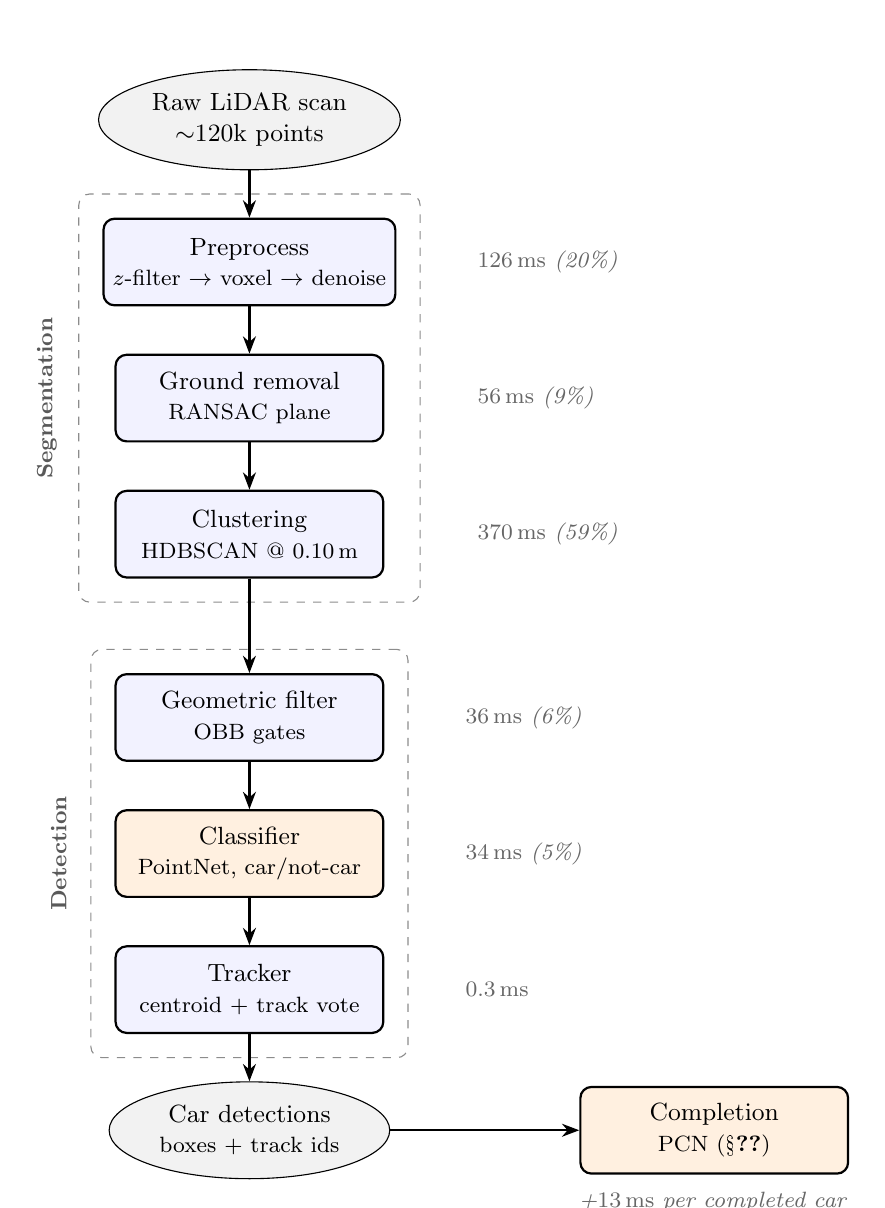
\begin{tikzpicture}[
      font=\small,
      node distance=6mm,
      stage/.style={
        draw, rounded corners, align=center,
        minimum width=34mm, minimum height=11mm,
        fill=blue!5, thick},
      learned/.style={stage, fill=orange!12},
      io/.style={draw, ellipse, align=center, fill=black!5,
        minimum width=28mm, minimum height=9mm},
      ms/.style={font=\footnotesize\itshape, text=black!60},
      arr/.style={-{Stealth[length=2.2mm]}, thick},
      grp/.style={draw=black!45, dashed, rounded corners, inner sep=3mm},
      grplab/.style={font=\footnotesize\bfseries, text=black!65},
    ]
    \node[io] (raw) {Raw LiDAR scan\\$\sim$120k points};
    \node[stage, below=of raw] (pre) {Preprocess\\{\footnotesize $z$-filter $\to$ voxel $\to$ denoise}};
    \node[stage, below=of pre] (ground) {Ground removal\\{\footnotesize RANSAC plane}};
    \node[stage, below=of ground] (cluster) {Clustering\\{\footnotesize HDBSCAN @ \SI{0.10}{\meter}}};
    \node[stage, below=12mm of cluster] (geo) {Geometric filter\\{\footnotesize OBB gates}};
    \node[learned, below=of geo] (clf) {Classifier\\{\footnotesize PointNet, car/not-car}};
    \node[stage, below=of clf] (track) {Tracker\\{\footnotesize centroid + track vote}};
    \node[io, below=of track] (out) {Car detections\\{\footnotesize boxes + track ids}};
    \node[learned, right=24mm of out] (comp) {Completion\\{\footnotesize PCN (\S\ref{ch:completion-method})}};

    \draw[arr] (raw) -- (pre);
    \draw[arr] (pre) -- (ground);
    \draw[arr] (ground) -- (cluster);
    \draw[arr] (cluster) -- (geo);
    \draw[arr] (geo) -- (clf);
    \draw[arr] (clf) -- (track);
    \draw[arr] (track) -- (out);
    \draw[arr] (out) -- (comp);

    % dashed phase blocks (segmentation: points -> clusters; detection: clusters -> cars)
    \begin{scope}[on background layer]
      \node[grp, fit=(pre)(ground)(cluster)] (segbox) {};
      \node[grp, fit=(geo)(clf)(track)] (detbox) {};
    \end{scope}
    \node[grplab, rotate=90] at ([xshift=-4mm]segbox.west) {Segmentation};
    \node[grplab, rotate=90] at ([xshift=-4mm]detbox.west) {Detection};

    % per-stage timing in one column, anchored to the phase-block right edge (uniform gap)
    \node[ms, anchor=west] at ([xshift=6mm]segbox.east|-pre)     {\SI{126}{\milli\second} (20\%)};
    \node[ms, anchor=west] at ([xshift=6mm]segbox.east|-ground)  {\SI{56}{\milli\second} (9\%)};
    \node[ms, anchor=west] at ([xshift=6mm]segbox.east|-cluster) {\SI{370}{\milli\second} (59\%)};
    \node[ms, anchor=west] at ([xshift=6mm]detbox.east|-geo)     {\SI{36}{\milli\second} (6\%)};
    \node[ms, anchor=west] at ([xshift=6mm]detbox.east|-clf)     {\SI{34}{\milli\second} (5\%)};
    \node[ms, anchor=west] at ([xshift=6mm]detbox.east|-track)   {\SI{0.3}{\milli\second}};
    \node[ms, below=1mm of comp.south, text width=34mm, align=center]
      {\footnotesize\itshape +\SI{13}{\milli\second} per completed car};
  \end{tikzpicture}
  \caption[Detection pipeline]{The detection pipeline, grouped into two phases (dashed): a
    \emph{segmentation} phase that turns a raw scan into clusters (preprocess, ground removal,
    clustering) and a \emph{detection} phase that turns clusters into tracked car boxes
    (geometric filter, classifier, tracker); the optional completion stage (right) runs off the
    tracked detections. Learned stages are shaded; all others are
    classical. Per-stage figures are mean wall-clock time on the full
    sequence~08 under the final (promoted) configuration
    (\num{4068} frames, AMD Ryzen 7 7800X3D + RTX 3070~Ti;
    \texttt{output/experiments/timing/timing\_seq08\_full\_n4068\_combined.json}), and are
    measured, not estimated. The total is
    \SI{623.5}{\milli\second\per\frame} ($\approx$\SI{1.6}{\fps}); the only learned
    \emph{per-frame} stage --- the classifier --- accounts for just
    \SI{34}{\milli\second} (\SI{5}{\percent}), and the classical clustering and
    ground-removal stages dominate. Completion runs off the tracked detections and
    is optional; it is learned, but its cost is per completed car, not per frame, so
    it does not enter this per-frame budget.}
  \label{fig:pipeline}
\end{figure}

The system is \emph{offline} by design: the tracker and the track-level filter
use the whole sequence, and real-time operation is out of scope. At
\SI{623.5}{\milli\second\per\frame} the pipeline is roughly \SI{1.6}{\fps}, an order
of magnitude below sensor rate; we characterise this cost honestly in the runtime
section of Chapter~\ref{ch:evaluation} rather than claiming real-time capability. The cost lives in the classical stages:
clustering alone is \SI{59}{\percent} of the frame budget, and the only learned
per-frame stage, the classifier, is just \SI{5}{\percent}. The expensive parts of this pipeline are
classical, not neural.

\subsection{Preprocessing: Filtering, Downsampling, and Denoising}
\label{sec:pipeline-preprocess}

Each raw scan (roughly \num{120000} points) passes through three cleaning steps
before any object reasoning:

\begin{enumerate}
  \item \textbf{Ground-height $z$-filter.} Points below
    $z = \SI{-2.0}{\meter}$ in the sensor frame are dropped. This removes the bulk
    of the road surface and any sub-ground noise cheaply, before the more
    expensive steps see them.
  \item \textbf{Voxel downsampling} at \SI{0.05}{\meter}. Points are collapsed to
    one representative per \SI{5}{\centi\meter} voxel, which both regularises the
    range-dependent density of LiDAR and cuts the point count by roughly an order
    of magnitude.
  \item \textbf{Statistical outlier removal.} Points whose mean distance to their
    \num{20} nearest neighbours exceeds \num{2.0} standard deviations of the
    local distribution are discarded, removing isolated speckle.
\end{enumerate}

The order of the last two steps is behaviour-changing. In the frozen configuration
(\texttt{voxel\_\allowbreak before\_\allowbreak denoise = True}) downsampling runs \emph{before}
denoising, so the statistical outlier test operates on roughly ten times fewer
points --- and on a regularised point set, which changes which points survive.
This ordering was adopted as part of the pipeline optimisation primarily
because it improves detection (discussed in Chapter~\ref{ch:evaluation}); its effect on the measured
denoising cost is small. It is behaviour-changing, so we flag it here rather than
presenting the two orderings as equivalent.
Preprocessing costs \SI{126}{\milli\second\per\frame} in total, split across the
$z$-filter (\SI{58}{\milli\second}), denoising (\SI{50}{\milli\second}), and
downsampling (\SI{18}{\milli\second}).

\subsection{Ground-Plane Removal by RANSAC}
\label{sec:pipeline-ground}

The dominant remaining structure after preprocessing is the ground plane, which
must be removed before clustering or it bridges every object into one component.
We fit a single plane with RANSAC: over \num{300} iterations, three points are
sampled, their plane computed, and inliers counted within
\SI{0.2}{\meter}; the best-supported plane is kept. The plane is
\emph{accepted only if its normal is near-vertical} --- the $z$-component of the
unit normal must exceed \num{0.5} --- so a spuriously-fitted vertical surface (a
wall, the side of a truck) cannot be mistaken for ground. If the check fails, no
points are removed and the whole cloud is passed on as objects; this fail-safe is
rare but prevents a bad plane fit from deleting real cars.

A single global plane is a deliberate simplification: it assumes the local ground
is approximately planar, which holds on the flat urban sequences used here but
would degrade on strong slopes. A grid-based ground model (Patchwork++-style) is
listed as future work, not a limitation we claim to have solved. The iteration
count was reduced from \num{1000} to \num{300} as part of the runtime optimisation after
confirming the plane fit converges well before \num{1000} iterations on this
data; the fit uses a fixed seed (\texttt{np.random.default\_rng(42)}) so ground
removal, and therefore the whole pipeline, is deterministic across runs. Ground
removal costs \SI{56}{\milli\second\per\frame} (\SI{9}{\percent} of the frame).

\subsection{Object-Candidate Clustering with HDBSCAN}
\label{sec:pipeline-cluster}

Non-ground points are grouped into object candidates with HDBSCAN, a
density-based hierarchical clusterer, using a minimum cluster size of \num{10}
and minimum samples of \num{5}. HDBSCAN is chosen over a fixed-radius method
because LiDAR density falls off with range: a single Euclidean radius that merges
nothing at \SI{5}{\meter} will over-segment at \SI{40}{\meter}. HDBSCAN's
variable-density hierarchy adapts to this without a hand-tuned radius schedule,
and Chapter~\ref{ch:evaluation} reports a controlled benchmark confirming it beats
DBSCAN and Euclidean extraction on recall at matched settings.

Two details of the frozen configuration are load-bearing. First, clustering runs
on a \emph{coarser} \SI{0.10}{\meter} voxel grid than the \SI{0.05}{\meter}
preprocessing grid: the object cloud is re-downsampled to \SI{0.10}{\meter},
HDBSCAN is run there, and the labels are propagated back to the full-resolution
points by nearest neighbour. This was adopted because the coarser
grid closes intra-car density gaps that otherwise cause a single car to split
into several clusters --- the central mechanism of the recall bottleneck analysed
in Section~\ref{sec:recall-analysis} (Figure~\ref{fig:clustering}) --- and it added \num{1655} true positives on the full sequence~08.
Second, HDBSCAN is by far the most expensive stage at
\SI{370}{\milli\second\per\frame} (\SI{59}{\percent} of the budget), because it is
superlinear in the point count; the coarse-grid trick is as much a speed measure
as an accuracy one. The clustering stage produces on average \num{45} candidate
clusters per frame.

\begin{figure}[H]
  \centering
  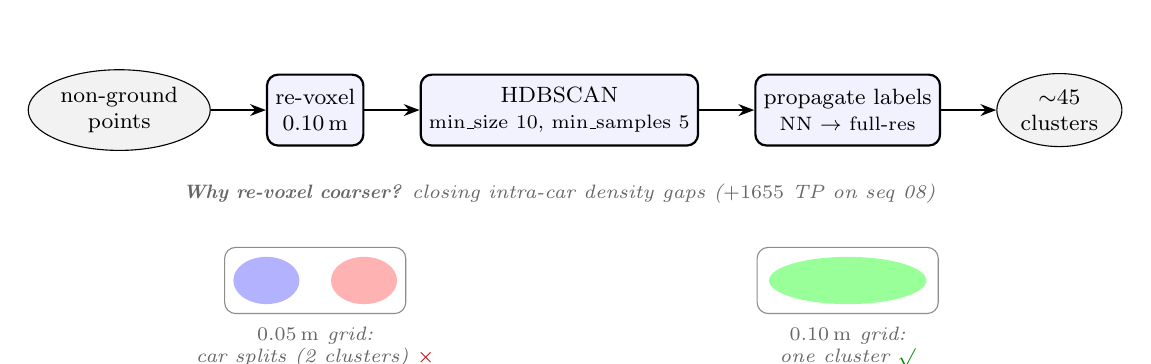
\begin{tikzpicture}[
      font=\footnotesize, node distance=5mm and 7mm,
      blk/.style={draw, rounded corners, align=center, fill=blue!5, thick,
        minimum height=9mm, inner sep=3pt},
      io/.style={draw, ellipse, align=center, fill=black!5, inner sep=2pt},
      arr/.style={-{Stealth[length=2mm]}, thick},
      note/.style={font=\scriptsize\itshape, text=black!60, align=center},
    ]
    % --- top: the clustering flow ---
    \node[io] (in) {non-ground\\points};
    \node[blk, right=of in] (vox) {re-voxel\\\SI{0.10}{\meter}};
    \node[blk, right=of vox] (hdb) {HDBSCAN\\{\scriptsize min\_size \num{10}, min\_samples \num{5}}};
    \node[blk, right=of hdb] (prop) {propagate labels\\{\scriptsize NN $\to$ full-res}};
    \node[io, right=of prop] (out) {$\sim$\num{45}\\clusters};
    \draw[arr] (in)--(vox); \draw[arr] (vox)--(hdb);
    \draw[arr] (hdb)--(prop); \draw[arr] (prop)--(out);

    % --- bottom: why the coarser grid (split vs whole) ---
    \node[note] (why) at ($(hdb.south)+(0,-6mm)$)
      {\textbf{Why re-voxel coarser?} closing intra-car density gaps ($+\num{1655}$ TP on seq~08)};
    \begin{scope}[shift={($(vox.south)+(0,-17mm)$)}]
      \draw[rounded corners, black!45] (-1.15,-0.42) rectangle (1.15,0.42);
      \fill[blue!30] (-0.62,0) ellipse (0.42 and 0.30);
      \fill[red!30]  (0.62,0)  ellipse (0.42 and 0.30);
      \node[note] at (0,-0.85) {\SI{0.05}{\meter} grid:\\car splits (2 clusters) {\textcolor{red!75!black}{$\times$}}};
    \end{scope}
    \begin{scope}[shift={($(prop.south)+(0,-17mm)$)}]
      \draw[rounded corners, black!45] (-1.15,-0.42) rectangle (1.15,0.42);
      \fill[green!40] (0,0) ellipse (1.0 and 0.30);
      \node[note] at (0,-0.85) {\SI{0.10}{\meter} grid:\\one cluster {\textcolor{green!55!black}{$\surd$}}};
    \end{scope}
  \end{tikzpicture}
  \caption[Clustering stage]{The clustering stage. Non-ground points are re-voxelised to a coarser
    \SI{0.10}{\meter} grid, clustered with HDBSCAN (density-adaptive, so a single car stays whole at
    both near and far range without a hand-tuned radius), and the cluster labels are propagated back to
    the full-resolution points by nearest neighbour. The coarser grid is load-bearing (bottom): on the
    \SI{0.05}{\meter} preprocessing grid intra-car density gaps split one car into several clusters,
    whereas the \SI{0.10}{\meter} grid closes them and keeps the car a single cluster --- worth
    \num{1655} true positives on sequence~08. HDBSCAN is the pipeline's most expensive stage at
    \SI{370}{\milli\second\per\frame} (\SI{59}{\percent}), so the coarse grid is also a speed measure.}
  \label{fig:clustering}
\end{figure}

\subsection{Geometric Filtering of Non-Car Clusters}
\label{sec:pipeline-geometric}

Most clusters are not cars: they are trees, poles, building facades, and
fragments. A geometric filter rejects clusters whose oriented bounding box (OBB)
is inconsistent with a car, using only cheap, interpretable shape gates. For each
cluster the OBB is computed and the cluster is kept only if it passes \emph{all}
of the following:

\begin{itemize}
  \item at least \num{15} points;
  \item OBB volume in $[\num{0.5}, \num{50}]\,\si{\meter\cubed}$;
  \item longest OBB extent $\leq \SI{6.0}{\meter}$, and the two largest extents
    above small floors (\SI{0.5}{} and \SI{0.4}{\meter}), rejecting slivers;
  \item box centre no more than \SI{1.5}{\meter} above the fitted ground plane,
    and vertical point span $\leq \SI{1.8}{\meter}$, rejecting tall structures;
  \item aspect ratio (longest\,/\,shortest extent) $\leq \num{6.0}$, rejecting
    thin walls and poles.
\end{itemize}

These bounds are generous car priors, not a tight car model --- they are meant to
remove obvious non-cars while leaving the fine car/not-car decision to the
learned classifier. The height gate is computed \emph{relative to the fitted
ground plane}, not to a fixed world height, so it is robust to the sensor not
being perfectly level. The filter costs \SI{36}{\milli\second\per\frame}
(\SI{6}{\percent}). Its individual gates are ablated in Chapter~\ref{ch:evaluation}; the stage is
high-recall and low-precision by construction, and the
classifier is what turns its survivors into precise detections.

\subsection{The Car / Not-Car Point Classifier}
\label{sec:pipeline-classifier}

Each surviving cluster is classified as \emph{car} or \emph{not-car} by a small
dual-branch PointNet (\texttt{src/\allowbreak classifier.py}). The binary decision
replaces
an earlier multi-class (car/bus/motorcycle) design that was dropped once the data
showed near-zero real bus and motorcycle instances, leaving the car-only detector
(Chapter~\ref{ch:introduction}).

\paragraph{Architecture.} The network has two branches
(Figure~\ref{fig:classifier}) and about \num{80000}
parameters --- deliberately small:
\begin{itemize}
  \item a \textbf{point branch} that takes \num{512} points (sampled or padded)
    normalised into the unit sphere, and applies shared per-point MLPs
    ($3 \to 64 \to 128 \to 256$) followed by a max-pool to a \num{256}-d shape
    descriptor;
  \item a \textbf{bounding-box branch} that takes an \num{8}-dimensional metric
    feature vector (sorted OBB extents, volume, two aspect ratios,
    $\log(1+\text{point count})$, vertical span), $z$-score normalised, through a
    small MLP to \num{32}-d.
\end{itemize}
The two are concatenated and passed through a small head
($288 \to 128 \to 2$) with dropout. The bounding-box branch is what re-injects
absolute metric scale, which the unit-sphere normalisation deliberately strips
from the point branch: a distant small car and a nearby one have the same
normalised shape but different real extents, and the metric branch is how the
network sees the difference. There are no T-Nets, since clusters already sit in a
consistent sensor frame.

\begin{figure}[H]
  \centering
  \resizebox{\linewidth}{!}{%
  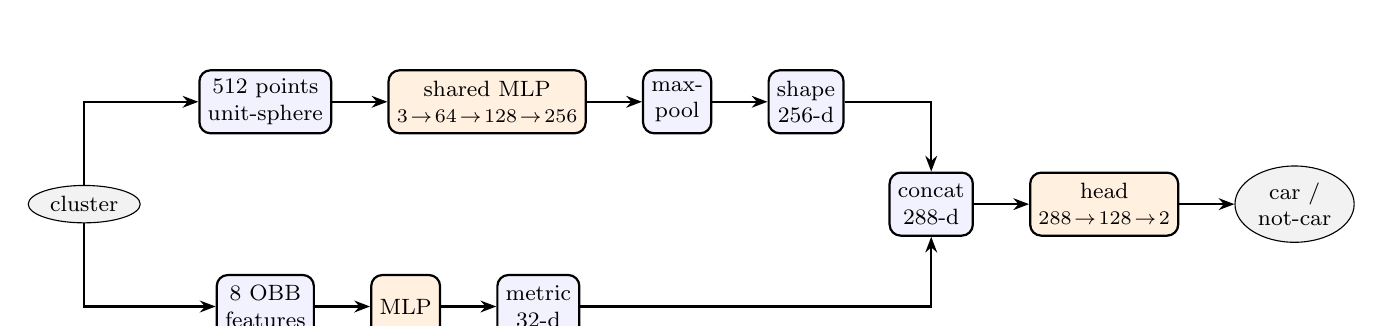
\begin{tikzpicture}[
      font=\footnotesize, node distance=6mm and 7mm,
      blk/.style={draw, rounded corners, align=center, fill=blue!5, thick,
        minimum height=8mm, inner sep=3pt},
      lrn/.style={blk, fill=orange!12},
      io/.style={draw, ellipse, align=center, fill=black!5, inner sep=2pt},
      arr/.style={-{Stealth[length=2mm]}, thick},
    ]
    \node[io] (cl) at (0,0) {cluster};
    \node[blk] (pts) at (2.3,1.3) {\num{512} points\\unit-sphere};
    \node[lrn, right=of pts] (pmlp) {shared MLP\\{\scriptsize $3\!\to\!64\!\to\!128\!\to\!256$}};
    \node[blk, right=of pmlp] (pool) {max-\\pool};
    \node[blk, right=of pool] (pd) {shape\\\num{256}-d};
    \node[blk] (feat) at (2.3,-1.3) {\num{8} OBB\\features};
    \node[lrn, right=of feat] (bmlp) {MLP};
    \node[blk, right=of bmlp] (bd) {metric\\\num{32}-d};
    \node[blk] (cat) at ($(pd.east)+(1.1,-1.3)$) {concat\\\num{288}-d};
    \node[lrn, right=of cat] (head) {head\\{\scriptsize $288\!\to\!128\!\to\!2$}};
    \node[io, right=of head] (out) {car /\\not-car};
    \draw[arr] (cl) |- (pts.west);
    \draw[arr] (cl) |- (feat.west);
    \draw[arr] (pts)--(pmlp); \draw[arr] (pmlp)--(pool); \draw[arr] (pool)--(pd);
    \draw[arr] (feat)--(bmlp); \draw[arr] (bmlp)--(bd);
    \draw[arr] (pd) -| (cat.north);
    \draw[arr] (bd) -| (cat.south);
    \draw[arr] (cat) -- (head);
    \draw[arr] (head) -- (out);
  \end{tikzpicture}%
  }
  \caption[Dual-branch classifier]{The dual-branch classifier (\texttt{src/classifier.py}), applied to one
    cluster. The \emph{point branch} takes \num{512} unit-sphere-normalised points
    through shared per-point MLPs and a max-pool to a \num{256}-d shape descriptor;
    the \emph{bounding-box branch} takes \num{8} metric shape features --- the
    absolute scale the sphere normalisation strips --- to \num{32}-d. The two are
    concatenated and passed through a small head to a car/not-car decision. Learned
    blocks are shaded.}
  \label{fig:classifier}
\end{figure}

\paragraph{Training data (mined, not hand-labelled).} The classifier is trained
on real LiDAR clusters mined automatically from SemanticKITTI
(\texttt{src/mine\_stage\_b.py}). For each training frame the pipeline's own
stages~1--5 are replayed, the ground-truth semantic labels are propagated onto the
surviving clusters by nearest neighbour, and each cluster is labelled \emph{car}
or \emph{not-car} by majority vote, keeping only clusters whose majority class
has purity $\geq \num{0.75}$. This yields \num{420333} training clusters
(sequences 00--07, 09, 10) and \num{130394} validation clusters (sequence~08),
with the intrinsic $\approx$21\,\%/79\,\% car/not-car imbalance handled by a
class-weighted loss. The key property is that the training clusters are produced
by the \emph{same} clustering and filtering the classifier meets at inference ---
including HDBSCAN splits and filter survivors --- so it learns on exactly the
distribution it must classify, at no manual-annotation cost.

\paragraph{Production checkpoint: trained from scratch.} The production classifier
is \texttt{stage\_b\_\allowbreak scratch\_\allowbreak best.pth}, trained on the
mined real clusters from
random initialisation (val macro-$F_1$ \num{0.9285}). An earlier
two-stage design first pretrained on synthetic ShapeNet partial renders
(``Stage~A'') and then fine-tuned on the real clusters (``Stage~B''). We report
the two-stage machinery in Chapter~\ref{ch:evaluation} as an \emph{ablation}, because a controlled
comparison showed the synthetic pretraining to be \emph{redundant}
given \num{420000} real clusters: the from-scratch classifier matches the
pretrained one (macro-$F_1$ \num{0.9285} vs.\ \num{0.9225}). The final pipeline
therefore uses the simpler from-scratch checkpoint, and the synthetic
pretraining, together with the finding that the sim-to-real gap is total and
symmetric, is presented as a negative result rather than as a
contribution. The classifier costs \SI{34}{\milli\second\per\frame} (about
\SI{0.75}{\milli\second} per cluster over the \num{45} clusters in a frame).

\paragraph{Training.} The from-scratch checkpoint is trained for \num{15} epochs
with Adam (learning rate \num{e-4}, weight decay \num{e-5}) and a step schedule
that halves the rate every \num{10} epochs, at batch size \num{64}. The loss is
cross-entropy weighted by inverse square-root class frequency (normalised to unit
mean), which offsets the intrinsic $\approx$21\,\%/79\,\% car/not-car imbalance
without resampling. Training clusters are augmented online with a random rotation
about the vertical axis and Gaussian jitter ($\sigma = \SI{0.005}{\meter}$); the
input is the \num{512}-point cluster of the architecture above. Runs are seeded
and the reported checkpoint is the epoch with the best validation macro-$F_1$
(\num{0.9285} on the sequence-08 validation clusters).

\subsection{Multi-Frame Tracking and Track-Level Filtering}
\label{sec:pipeline-tracker}

Detections are linked across frames by a centroid tracker
(\texttt{src/tracker.py}). Each frame, current detections are matched to existing
tracks by solving a Hungarian assignment on the pairwise centroid-distance
matrix; matches beyond \SI{2.0}{\meter} are rejected, unmatched detections start
new tracks, and a track that goes unmatched for more than \num{5} consecutive
frames is retired. This is an offline, centroid-only tracker --- no motion model,
no appearance --- which is adequate here because detection, not association, is
the bottleneck; an IoU-based (SORT-style) tracker is listed as future work.

The tracker also enables a \emph{track-level filter} that improves precision
(Figure~\ref{fig:tracker}).
Each detection carries the classifier's per-frame label; a track is accepted as a
car only if, across its lifetime, it collected at least \num{2} non-rejected
votes, those known votes are a majority of its votes
($\geq \num{0.5}$), and they agree on a single class. A cluster that the
classifier flickers on --- a car in one frame, not-car in the next --- is thus
resolved by temporal majority rather than trusted per frame. Because this filter
consults the whole track, it is an offline post-processing step, consistent with
the offline scope of the system; its contribution is isolated as an ablation row
in Chapter~\ref{ch:evaluation}. The tracker itself is effectively free at
\SI{0.3}{\milli\second\per\frame}.

\begin{figure}[H]
  \centering
  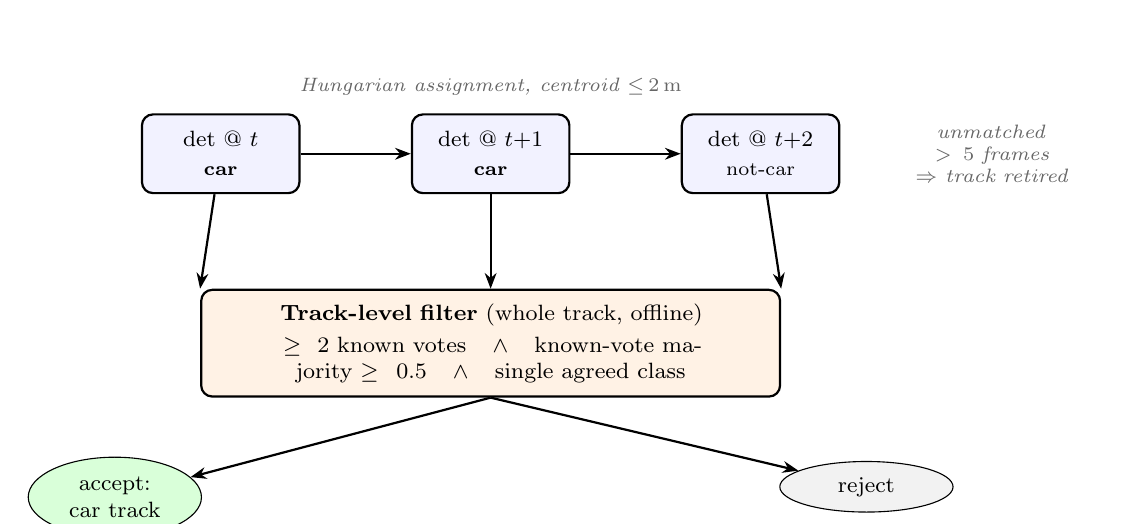
\begin{tikzpicture}[
      font=\footnotesize, node distance=6mm and 14mm,
      det/.style={draw, rounded corners, align=center, fill=blue!5, thick,
        minimum height=10mm, minimum width=20mm, inner sep=3pt},
      dec/.style={draw, rounded corners, align=center, fill=orange!10, thick, inner sep=5pt},
      res/.style={draw, ellipse, align=center, inner sep=3pt, minimum width=22mm},
      arr/.style={-{Stealth[length=2mm]}, thick},
      lbl/.style={font=\scriptsize\itshape, text=black!60, align=center},
    ]
    % one track's per-frame detections, linked by centroid association
    \node[det] (d1) {det @ $t$\\[1pt]{\scriptsize\bfseries car}};
    \node[det, right=of d1] (d2) {det @ $t{+}1$\\[1pt]{\scriptsize\bfseries car}};
    \node[det, right=of d2] (d3) {det @ $t{+}2$\\[1pt]{\scriptsize not-car}};
    \draw[arr] (d1)--(d2);
    \draw[arr] (d2)--(d3);
    \node[lbl, above=1mm of d2] {Hungarian assignment, centroid $\le$\,\SI{2}{\meter}};
    \node[lbl, right=6mm of d3, text width=24mm] (ret)
      {unmatched $>\num{5}$ frames\\$\Rightarrow$ track retired};

    % track-level filter over the whole vote sequence
    \node[dec, below=12mm of d2, text width=70mm] (filt)
      {\textbf{Track-level filter} (whole track, offline)\\[2pt]
       $\ge \num{2}$ known votes \;\, $\wedge$ \;\, known-vote majority $\ge \num{0.5}$
       \;\, $\wedge$ \;\, single agreed class};
    \draw[arr] (d1) -- (filt.north west);
    \draw[arr] (d2) -- (filt.north);
    \draw[arr] (d3) -- (filt.north east);

    \node[res, fill=green!15, below left=9mm and 3mm of filt] (acc) {accept:\\car track};
    \node[res, fill=black!5, below right=9mm and 3mm of filt] (rej) {reject};
    \draw[arr] (filt.south) -- (acc);
    \draw[arr] (filt.south) -- (rej);
  \end{tikzpicture}
  \caption[Tracker and track-level filter]{The tracker and track-level filter. Per-frame detections
    are linked into tracks by Hungarian assignment on centroid distance (matches beyond \SI{2}{\meter}
    rejected; a track unmatched for more than \num{5} frames retired). The track-level filter then
    resolves each track over its \emph{whole} vote sequence rather than per frame: a track is accepted as
    a car only with at least \num{2} known votes, a known-vote majority of at least \num{0.5}, and
    agreement on a single class. In the worked example the votes \{car, car, not-car\} clear all three
    gates, so a classifier flicker in one frame is overruled by temporal majority. Both steps are
    offline; the tracker costs \SI{0.3}{\milli\second\per\frame}.}
  \label{fig:tracker}
\end{figure}

\subsection{The Frozen Pipeline Configuration}
\label{sec:pipeline-config}

Table~\ref{tab:pipeline-config} lists the frozen parameter values that produce
every number in this thesis. They are the committed \texttt{PIPELINE\_CONFIG} and
were not altered to obtain any reported result.

\begin{table}[H]
  \centering
  \caption[Frozen pipeline configuration]{Frozen pipeline configuration (\texttt{src/pipeline.py}). These values
    were fixed before the write-up; no reported number was produced by changing
    them.}
  \label{tab:pipeline-config}
  \begin{tabular}{lll}
    \toprule
    Stage & Parameter & Value \\
    \midrule
    Preprocess & $z$-filter threshold & \SI{-2.0}{\meter} \\
               & voxel size & \SI{0.05}{\meter} \\
               & denoise neighbours / std-ratio & \num{20} / \num{2.0} \\
               & voxel before denoise & true \\
    \midrule
    Ground     & RANSAC iterations & \num{300} \\
               & inlier distance & \SI{0.2}{\meter} \\
               & min.\ normal $z$ & \num{0.5} \\
    \midrule
    Clustering & method & HDBSCAN \\
               & min.\ cluster size / min.\ samples & \num{10} / \num{5} \\
               & clustering voxel size & \SI{0.10}{\meter} \\
    \midrule
    Geometric  & min.\ points & \num{15} \\
               & volume range & $[\num{0.5}, \num{50}]\,\si{\meter\cubed}$ \\
               & max.\ longest extent & \SI{6.0}{\meter} \\
               & max.\ height above ground & \SI{1.5}{\meter} \\
               & max.\ vertical span & \SI{1.8}{\meter} \\
               & max.\ aspect ratio & \num{6.0} \\
    \midrule
    Classifier & checkpoint & \texttt{stage\_b\_scratch\_best.pth} \\
               & input points & \num{512} \\
    \midrule
    Tracker    & max.\ match distance & \SI{2.0}{\meter} \\
               & max.\ disappeared frames & \num{5} \\
               & min.\ track length & \num{2} \\
               & min.\ known votes / ratio & \num{2} / \num{0.5} \\
    \bottomrule
  \end{tabular}
\end{table}

The completion stage that operates on the tracked car detections
(Figure~\ref{fig:pipeline}, right) is the subject of Section~\ref{ch:completion-method}; the evaluation of
the detections themselves is Chapter~\ref{ch:evaluation}.


%% ===== merged from sec_6_completion_method.tex ===== %%

% Point-Cloud Completion: Method (clean-method-first; false starts gathered in a
% closing "Negative results and lessons" subsection). Folds under Chapter 3.
%
% Scope: this section is the completion METHOD and the debugging narrative that
% produced it. The completion RESULTS (donor metric, box metric, held-out
% replication, movers) live in Chapter 4 (Evaluation); here we only state each fix's headline
% effect and defer the full evaluation.
%
% Honesty-phrasing rules applied (personal_agenda P1):
%   - domain-gap failures (#15-19) and Step 1c (#45) presented as FINDINGS, not
%     apologies; #26 inference bug presented as a debugging lesson.
%   - final path = per-car length estimate ON, Step 1c flags OFF.
%   - 23% fallback (#41) stated as a live limitation.
%   - measured vs inferred tiers marked; numbers traceable to findings/artifacts.
%
% Figures (all embedded via \graphicspath from the gitignored output/ tree;
% regenerable from the named scripts):
%   Fig 6.1 fig61_partial_compare.py    -> fig61_partials/       (naive vs KITTI-like partial)
%   Fig 6.2 fig62_box_overlay.py        -> fig62_deblob/box_overlay_deblob_08.png
%           (BEV old vs corrected completion box vs amodal GT; reconstructs the
%            retired PCA+partial-radius normalization, touches nothing frozen)
%   Fig 6.3 viz_completion.py           -> completion_shape_08.png (final output, output/08)
% Floats set [htbp]. Draft-grade renders; may get a cosmetic restyle in the figure pass.
%
\section{Object Completion}
\label{ch:completion-method}

This part of the method takes each detected car and \emph{completes} it:
from the one-sided, partial cluster a single LiDAR frame observes, it predicts
the full car surface. The section presents the finished method in the order a
cluster passes through it --- the network, its training data, the inference-time
normalisation, the input gate, and the length geometry --- and then, separately,
gathers the negative results and lessons that shaped it
(Section~\ref{sec:completion-lessons}). Those false starts are of independent value
--- one is the motivating case for a project-wide rule --- so they are reported as
findings rather than smoothed over, but they are kept out of the method description
so that reads as what the pipeline does, not as how it was arrived at. The scientific
content here is not the network, a standard Point Completion Network (PCN) used off the
shelf, but the data it is trained on and the geometry by which a real partial is
presented to it. The evaluation of the finished method --- whether it adds genuinely
unseen surface, and whether that generalises --- is the subject of
Section~\ref{sec:donor-validation}; here we state each step's headline effect and defer
the rest.

\subsection{Completion Targets: Single-Frame Car Clusters}
\label{sec:completion-what}

Completion runs on the tracked car detections of Section~\ref{sec:meth-detection}. The input is a
\emph{single-frame} cluster in the sensor frame, not the accumulated multi-frame
track. This is a deliberate choice with an evidence basis: accumulating a moving car over many frames produces a
motion smear up to several metres long, which is neither a valid completion
target nor matchable to a car shape. A single frame is one clean, if partial,
observation. The value proposition --- that completing this partial improves the
car's amodal box and recovers surface the frame never saw --- is what Section~\ref{sec:donor-validation}
measures; this section is how the completion is produced.

\subsection{The Completion Network (PCN)}
\label{sec:completion-pcn}

We use PCN (Yuan et al., 2018), an encoder--decoder for point clouds
(\texttt{src/pcn.py}; Figure~\ref{fig:pcn}). The encoder is a stacked PointNet: shared per-point MLPs
lift each point to a local feature, a max-pool summarises the whole cloud into a
global vector, that global vector is concatenated back onto every point, and a
second MLP-plus-max-pool stage produces a single \num{1024}-dimensional shape
embedding. The decoder is coarse-to-fine: a fully-connected stage predicts
\num{1024} coarse seed points, then a \emph{grid-folding} stage attaches a small
2D grid patch to each seed and learns to fold it into local surface geometry,
densifying the coarse skeleton into the final cloud. Training minimises a
two-term Chamfer loss, $\mathrm{CD}_{\text{coarse}} + 0.5\,\mathrm{CD}_{\text{fine}}$;
the fine term is down-weighted so the coarse skeleton is learned first. At
inference the partial is subsampled to \num{256} points before it enters the
encoder.

\begin{figure}[H]
  \centering
  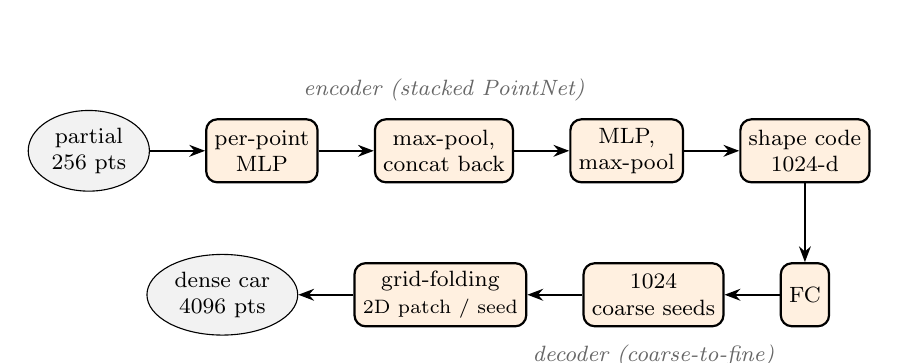
\begin{tikzpicture}[
      font=\footnotesize, node distance=6mm and 7mm,
      blk/.style={draw, rounded corners, align=center, fill=orange!12, thick,
        minimum height=8mm, inner sep=3pt},
      io/.style={draw, ellipse, align=center, fill=black!5, inner sep=2pt},
      arr/.style={-{Stealth[length=2mm]}, thick},
      lbl/.style={font=\footnotesize\itshape, text=black!60},
    ]
    \node[io] (in) {partial\\\num{256} pts};
    \node[blk, right=of in] (ppm) {per-point\\MLP};
    \node[blk, right=of ppm] (mp1) {max-pool,\\concat back};
    \node[blk, right=of mp1] (mp2) {MLP,\\max-pool};
    \node[blk, right=of mp2] (emb) {shape code\\\num{1024}-d};
    \node[blk, below=10mm of emb] (fc) {FC};
    \node[blk, left=of fc] (coarse) {\num{1024}\\coarse seeds};
    \node[blk, left=of coarse] (fold) {grid-folding\\{\scriptsize 2D patch / seed}};
    \node[io, left=of fold] (out) {dense car\\\num{4096} pts};
    \draw[arr] (in)--(ppm); \draw[arr] (ppm)--(mp1); \draw[arr] (mp1)--(mp2);
    \draw[arr] (mp2)--(emb); \draw[arr] (emb)--(fc); \draw[arr] (fc)--(coarse);
    \draw[arr] (coarse)--(fold); \draw[arr] (fold)--(out);
    \node[lbl, above=1mm of mp1] {encoder (stacked PointNet)};
    \node[lbl, below=1mm of coarse] {decoder (coarse-to-fine)};
  \end{tikzpicture}
  \caption[Completion network (PCN)]{The completion network (PCN, \texttt{src/pcn.py}). A stacked-PointNet
    encoder maps the \num{256}-point partial to a \num{1024}-d global shape code;
    a coarse-to-fine decoder predicts \num{1024} seed points and folds a small 2D
    grid patch onto each to produce the dense \num{4096}-point car. Every block is
    learned; the architecture is used off the shelf and unmodified.}
  \label{fig:pcn}
\end{figure}

The architecture is not a contribution and was not modified; the controlled comparison
against PoinTr that justifies keeping PCN --- a small synthetic edge and equivalent
real-data behaviour --- is reported with the completion ablations
(Section~\ref{sec:abl-completion}). What makes PCN
work on real cars is not the weights but the two subsections that follow: the
distribution of partials it is trained on, and the frame a real partial is normalised
into at inference.

\subsection{Training Data: KITTI-Like Partials}
\label{sec:completion-kittilike}

PCN is trained on synthetic partials, and those partials must match the distribution
of the real clusters it meets at inference or the network sees a different input at
test time than it was trained on. A derisk study comparing candidate partial
generators against real seq-08 clusters
(\texttt{scratchpad/derisk\_synth\_vs\_real.py}) isolated three properties a naive
generator gets wrong: it sampled a dense pinhole depth render, skipped the
\SI{0.05}{\meter} voxelisation and ground removal the real input has been through, and
added range-proportional noise (up to \SI{0.15}{\meter} at \SI{30}{\meter}) that
washed out the scan-ring banding real Velodyne data shows.

The generator used (\texttt{\_render\_kitti\_like} in \texttt{src/train\_pcn.py}) makes the synthetic partial match the real one: it orients the
ShapeNet car to gravity, casts a single HDL-64E viewpoint (64 elevation beams,
\SI{0.09}{\degree} horizontal resolution) from a sensor at \SI{1.73}{\meter} and
a sampled range of \SIrange{8}{30}{\meter}, adds small \emph{absolute} noise
(\SI{0.015}{\meter}), voxelises at \SI{0.05}{\meter} to match the pipeline, and
removes points within \SI{0.30}{\meter} of the ground plane. The dense complete
mesh sample remains the target. PCN retrained on these partials
(\texttt{pcn\_kitti\_best.pth}, best val loss \num{0.1246}) is in-distribution
with the real input, and on a held-out synthetic set produces clean cars, not
blobs (Chamfer \SI{0.16}{\meter}, F-score@\SI{0.1}{\meter} \num{0.76}).
Figure~\ref{fig:kitti-like-partial} contrasts the naive and KITTI-like partials
for the same ShapeNet car.

\paragraph{Training.} PCN is trained on the KITTI-like synthetic partials (input
\num{256} points, target the dense mesh sample) for \num{100} epochs with Adam
(learning rate \num{e-4}, weight decay \num{e-6}) and a step schedule that halves
the rate every \num{40} epochs, at batch size \num{8}, minimising the two-term
Chamfer loss above. No real cars enter training; the reported checkpoint
(\texttt{pcn\_kitti\_best.pth}) is the best-validation-loss epoch (\num{0.1246}).
The subsequent geometry work is all inference-time and does not retrain the
network.

\begin{figure}[htbp]
  \centering
  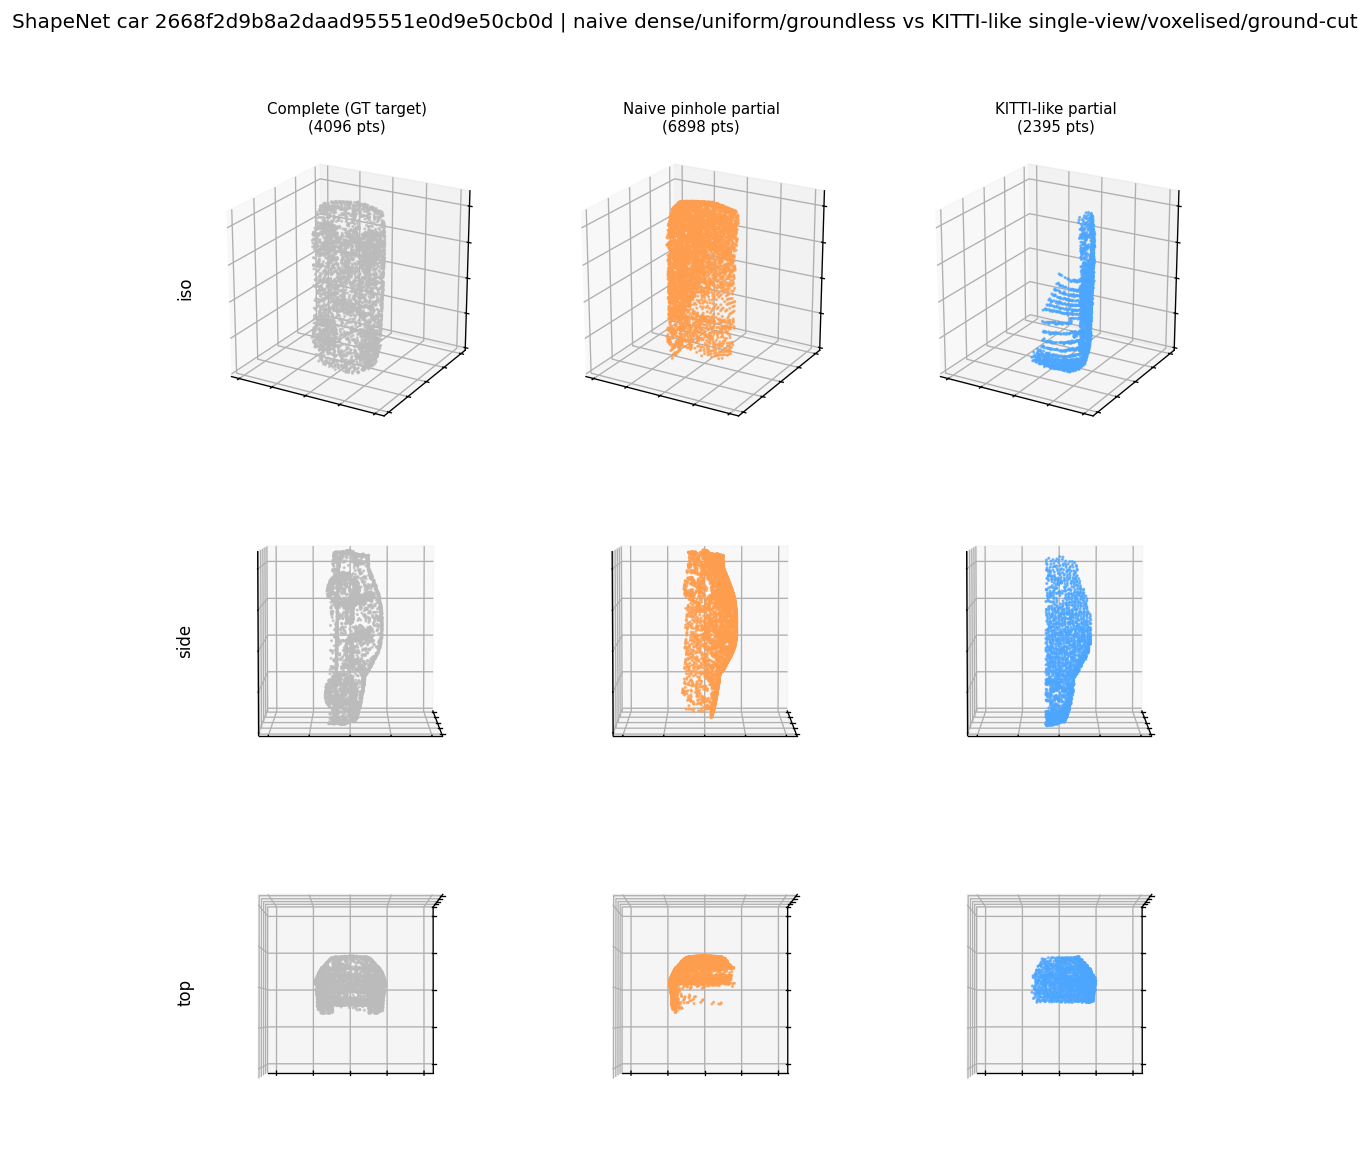
\includegraphics[width=\linewidth]{fig61_partials/partials_2668f2d9b8a2daad95551e0d9e50cb0d.png}
  \caption[Training-input distribution]{The training-input distribution: one ShapeNet car in
    three views, with its complete-surface target (left, grey) and two candidate
    training \emph{inputs}. The naive pinhole partial (centre, orange) is dense and
    uniform; the KITTI-like partial (right, blue) reproduces what real LiDAR
    delivers --- scan-ring banding, single-viewpoint coverage, \SI{0.05}{\meter}
    voxelisation, and the ground cut. Neither is a completion output; ``better''
    here means closer to the real input distribution, not more complete. Training on
    the KITTI-like distribution is what keeps the network in-distribution on real data.}
  \label{fig:kitti-like-partial}
\end{figure}

\subsection{Inference-Time Partial Normalisation}
\label{sec:completion-normalisation}

PCN is trained on shapes expressed in a fixed canonical car frame, centred on the
true car centre and scaled by the true car radius, so at inference a real partial
must be mapped into that \emph{same} frame before it is completed --- anything else
hands the network a normalisation it never saw during training. Reconstructing that
frame from a one-sided partial is non-trivial, because a partial reveals neither the
true centre nor the true radius directly. The inference path
(\texttt{estimate\_canonical\_frame}) reconstructs it in three steps:

\begin{itemize}
  \item \textbf{Reorientation.} The sensor frame is rotated into the canonical
    car frame (X${}={}$width, Y${}={}$up, Z${}={}$length): gravity maps to the
    up axis, and the horizontal heading axis maps to length. Heading comes from the
    L-shape footprint fit (Section~\ref{sec:completion-lshape}), not a principal-axis
    alignment.
  \item \textbf{Full-car centre estimate.} A one-sided partial's bounding-box
    centre is not the car centre, so the centre is corrected on each axis: shift
    \emph{down} to undo the upward bias from the ground cut (the dominant
    correction, \SI{0.25}{\meter}); push \emph{outward} along width toward the
    occluded far side to a half-car-width prior (\SI{1.9}{\meter}); and push
    along length toward the occluded far end (Section~\ref{sec:completion-length}).
  \item \textbf{Scale.} Normalise by the maximum point-to-centre distance divided
    by a fixed scale correction (\num{1.137}), the calibrated ratio between a
    one-sided partial radius and the true car radius.
\end{itemize}

With this path the same real seq-08 clusters recover the correct pose and scale; the
ablation isolating this normalisation against a naive partial-frame alternative, and the
box-overlap gains it produces, is reported with the completion ablations
(Section~\ref{sec:abl-completion}). Viewed in the
canonical car frame, the corrected completions are recognisably car-shaped: they
recover the car footprint in bird's-eye view and a rough side silhouette
(roofline included) even from very sparse input --- a clean car footprint from a
\num{64}-point cluster in the extreme case. We are nonetheless careful about the
strength of the claim: crispness varies with input density (cleaner on
well-observed cars, blobbier on the sparsest), and a completion is a filled
\num{4096}-point cloud rather than a CAD-clean surface. The sharpest completions
are the \emph{in-distribution synthetic} ones of
Section~\ref{sec:completion-kittilike} (Chamfer \SI{0.16}{\meter}); on real data
the normalisation's value is corrected geometry --- pose, scale, and the
surface-coverage gains quantified in Section~\ref{sec:donor-validation}. A calibration study on
synthetic cars further identified the residual dominant error as
\emph{centre estimation}, not scale --- which is what motivates the geometry work
in the rest of this section.

\subsection{L-Shape Gating of Completion Inputs}
\label{sec:completion-lshape}

Even with correct normalisation, some clusters cannot complete into a plausible
car because the \emph{input} is not one car: HDBSCAN fragments (part of a car) and
merges (two cars, or a \SI{90}{\degree} heading error) both feed the completion
network implausible input. To detect them we fit the cluster's ground-plane footprint with a
search-based L-shape fit (Zhang et al., 2017), which scores edge adherence over
candidate yaw angles and stays well-defined on near-square footprints where PCA
degenerates. The fitted footprint gives an input-quality gate: a
cluster is rejected as a fragment if its fitted length is below \SI{2.7}{\meter},
or as a merge if its fitted width exceeds \SI{2.3}{\meter}.

On seq-08 (\texttt{scratchpad/ab\_heading.py}) \emph{every} implausible completion
originated from a fragment or merge input, so the gate's effect on completion quality
is a clean ablation, reported in Section~\ref{sec:abl-completion}. An honest secondary
finding from the same study: the L-shape heading itself is neutral against plain PCA on
real data --- the fit earns its place by \emph{detecting bad inputs}, not by giving a
better heading.

\subsection{Per-Car Length Estimation}
\label{sec:completion-length}

The canonical-frame centre estimate re-centres the occluded lateral side and the
ground cut, but a partial truncated at the occluded far \emph{end} is normalised
around its observed near portion, so PCN's output stops short of the far end. The
donor metric of Section~\ref{sec:donor-validation} confirmed the far end as the single worst-covered
region. Two successive fixes address it, both inference-only (no retraining).

\paragraph{The fixed length prior.} A longitudinal, extend-only
push mirrors the width prior along the length axis: the centre is pushed toward
the occluded far end so the completion reaches an assumed full car length of
\SI{4.14}{\meter} (the real amodal-GT median). This more than doubled far-end
coverage on the donor metric and reversed the box-length regression (signed
$\Delta L$ \SI{-0.44}{}$\to$\SI{-0.32}{\meter}). A larger \SI{4.5}{\meter} prior
was rejected because it broke the hallucination guard by over-extending genuinely
compact cars.

\paragraph{The per-car estimate.} A single \SI{4.14}{\meter}
prior is a population median, so it is wrong in both tails --- it over-extends
compact cars and under-extends long ones. It is replaced by a per-car length,
\texttt{track\_length\_estimate}: the \nth{90} percentile of the car's own
gate-passed footprint-length fits, plus a \SI{0.12}{\meter} bias correction,
falling back to the fixed prior when a track has fewer than \num{5} gate-passed
frames. The estimator was chosen offline against amodal GT with no PCN inference:
a length-from-width shortcut is impossible (the correlation between true length
and width is \num{0.018}), and the aggregate must be a \emph{quantile}, not the
maximum, because a single contaminated L-shape fit sets the maximum. This is a
per-track quantity, so the pipeline (which owns the track) computes it and passes
it in; the completion module itself stays stateless. It removes the compact
over-extension (compact signed $\Delta L$ \SI{+0.295}{}$\to$\SI{+0.063}{\meter})
and improves the box metric overall (BEV IoU \num{0.747}$\to$\num{0.771}), at a
measured cost in pooled donor coverage that Section~\ref{sec:donor-validation} reports in full.

\paragraph{Limitation.} The fallback is not rare: on the
regenerated seq-08 output, \num{119} of \num{518} completed tracks
(\SI{23}{\percent}) fell back to the fixed prior because they had fewer than five
gate-passed frames. This is above a comfortable threshold and is stated as a live
limitation, not a solved problem; it is revisited in the discussion.

\subsection{The End-to-End Completion Path}
\label{sec:completion-summary}

To summarise, a single-frame car cluster is completed by: fitting its footprint
and rejecting fragments and merges (L-shape gate); reorienting it into the
canonical car frame with no PCA; estimating the full-car centre (down-shift for
the ground cut, width prior for the occluded side, per-car length estimate for
the occluded far end); normalising by the scale-corrected radius; running the
KITTI-like-trained PCN; and rotating the output back to the sensor frame. Every
step is inference-time geometry except the one-off retraining on KITTI-like
partials; no step fine-tunes on the evaluation cars.

Figure~\ref{fig:completion-shape} shows what this path produces on real seq-08
cars across the input-density range, in the canonical car frame. The completed
cloud (green) fills the car footprint and a rough side silhouette that the
single-frame partial (blue) leaves one-sided --- recognisably car-shaped down to a
\num{64}-point input, with fitted dimensions in the expected car range
($L \approx \SI{4.2}{\meter}$, $W \approx \SI{1.9}{\meter}$,
$H \approx \SI{1.6}{\meter}$ on the well-observed cars). Consistent with the
caveats above, the sparsest inputs complete more coarsely and can inflate the
width (Section~\ref{sec:donor-validation}), and the clouds are filled rather than CAD-clean;
the point here is qualitative shape, with the quantitative real-data assessment ---
whether the completion adds genuinely unseen surface, and whether that survives a
pre-registered held-out replication --- being what Section~\ref{sec:donor-validation} sets out to measure.

\begin{figure}[htbp]
  \centering
  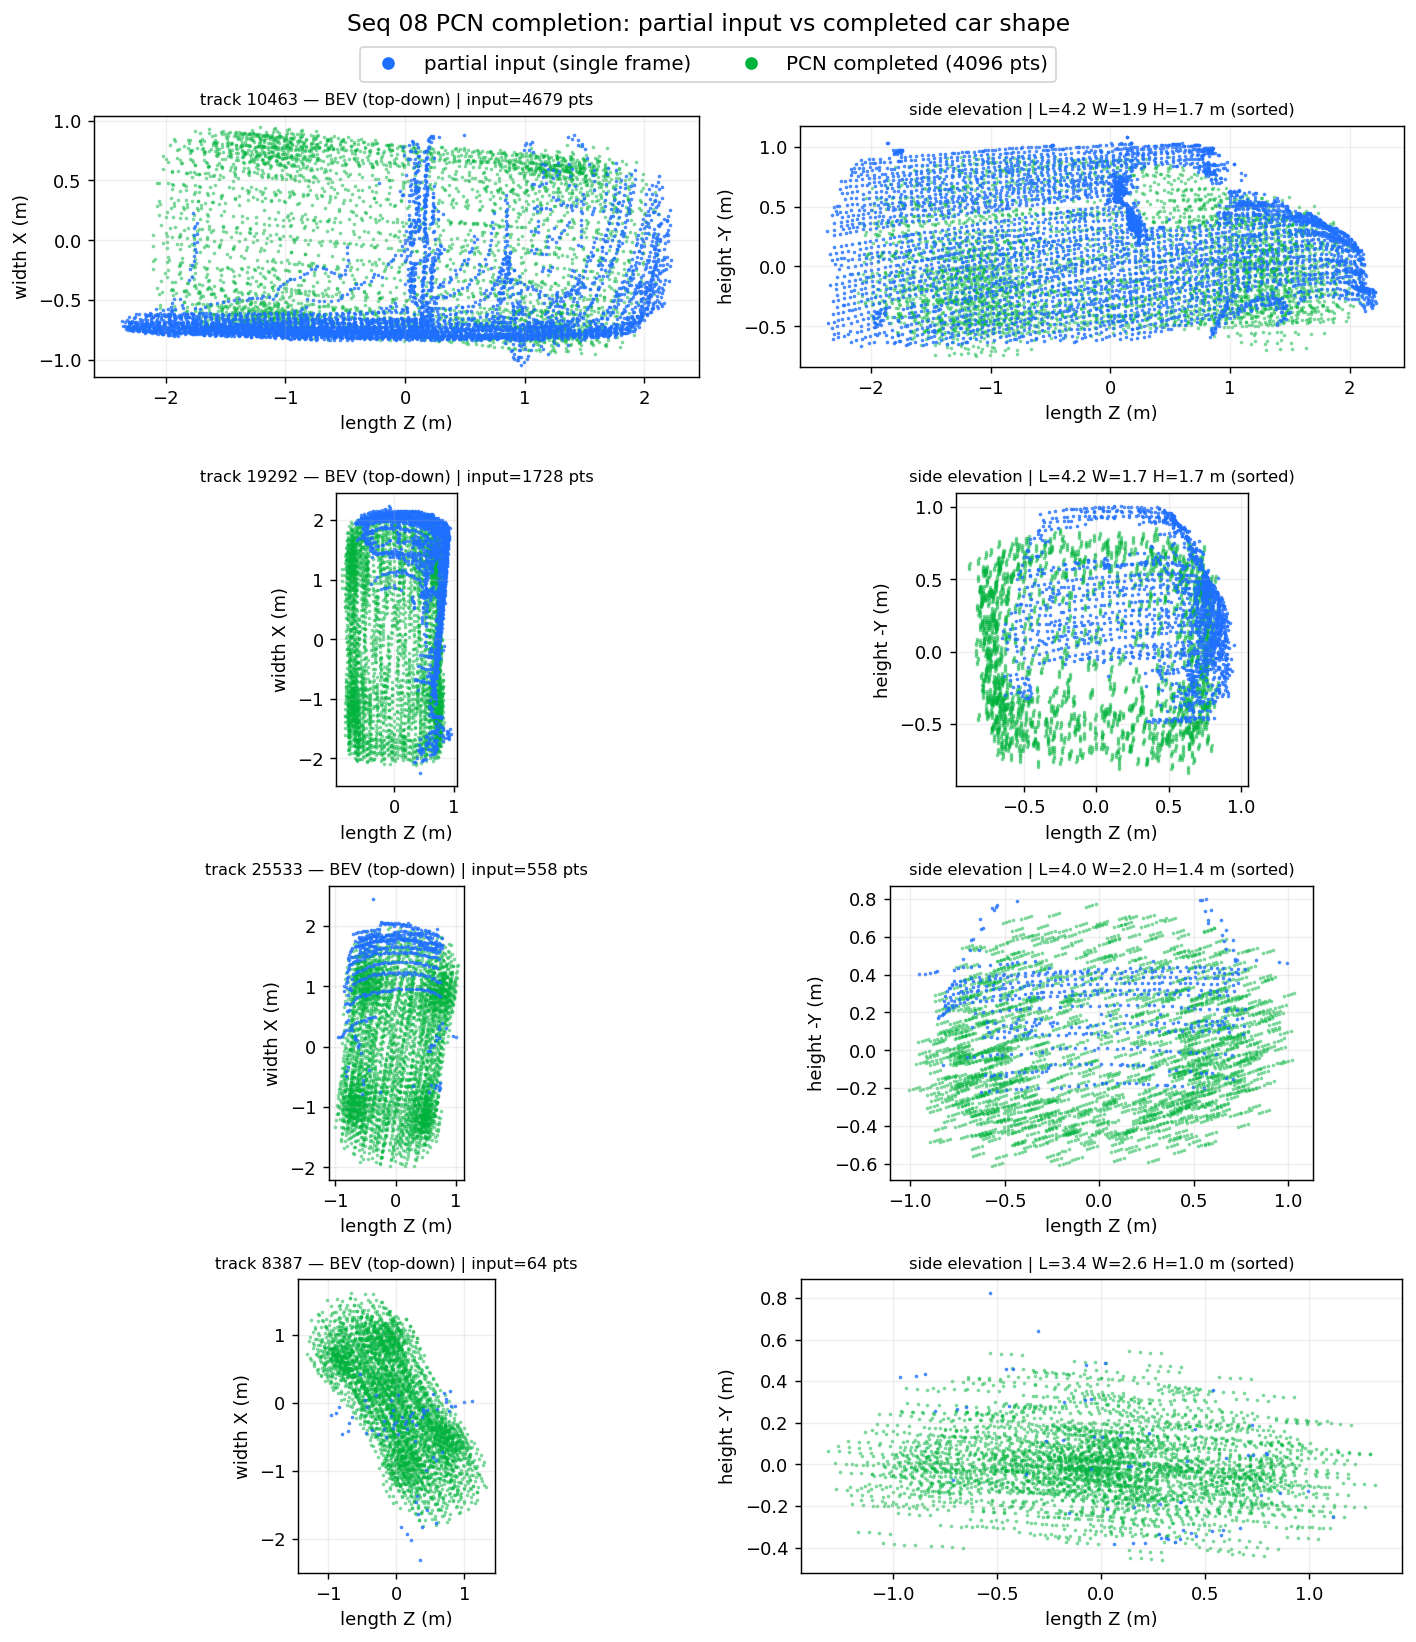
\includegraphics[width=\linewidth]{completion_shape_08.png}
  \caption[Completions on real seq-08 cars]{What the final completion path produces on real seq-08 cars, four
    tracks spanning the input-density range (\num{4679} down to \num{64} input
    points), each in the canonical car frame: bird's-eye view (left of each pair)
    and side elevation (right). Blue is the single-frame partial input, green the
    PCN completion. The completion recovers the full car footprint and a rough
    roofline silhouette from a one-sided partial; crispness and dimensional
    accuracy degrade on the sparsest inputs (the \num{64}-point car shows the
    width inflation discussed in Section~\ref{sec:donor-validation}). Rendered by
    \texttt{scratchpad/viz\_completion.py} from the final-config \texttt{output/08}.}
  \label{fig:completion-shape}
\end{figure}

\subsection{Negative Results and Lessons}
\label{sec:completion-lessons}

The method above was not reached in one step. Two false starts shaped it, and each
carries a lesson worth stating in its own right rather than smoothing over. They are
gathered here so that the method description reads as what the pipeline does. A third
intervention that was tried and rejected --- a length-dependent far-end
compensation --- is reported as a completion ablation
(Section~\ref{sec:abl-completion}).

\paragraph{The blobs were not a synthetic-data problem.}
\label{sec:completion-domaingap}
The first attempts to run PCN on real cars all produced ``blobs'' --- rounded,
car-sized clouds with no recognisable car structure. This was initially attributed to
the training data being synthetic, and the response was a series of sim-to-real
remedies: LiDAR-noise augmentation of the synthetic partials, and real-data
fine-tuning. None of them fixed the blobs, and the fine-tuning attempt is recorded as
a negative result --- on this data, fine-tuning PCN on mined real pairs did not recover
real-car geometry. The blobs had two causes, and neither was the network weights: the
training-input distribution (Section~\ref{sec:completion-kittilike}) and the inference
normalisation (Section~\ref{sec:completion-normalisation}), the two method steps above.
The lesson is to suspect the data and the input pipeline before the model.

\paragraph{Train and inference semantics must match.}
\label{sec:completion-inferencebug}
Even after retraining on KITTI-like partials, real clusters still blobbed, and the
cause is the sharper lesson. An earlier inference path normalised each real partial by
a 3D PCA frame and the \emph{partial's} own centroid and radius --- a normalisation the
model had never seen, since it was trained in the canonical car frame of
Section~\ref{sec:completion-normalisation}. This silent train/inference mismatch alone
produced blobs, and it did so for \emph{every} checkpoint, including in-distribution
synthetic ones (it worsened Chamfer by roughly \num{3.5}$\times$ even where the model
is otherwise clean). Because the two frames each looked internally reasonable, the
divergence was invisible until measured. This incident is the motivating example for
the project's rule that any external integration or reuse gets a written semantics map
--- coordinate frame, centring, and scale conventions --- reconciled before code is
run.

\section{The Donor-Frame Completion Metric}
\label{sec:donor-metric}

Evaluating the completion output requires a metric, and on real LiDAR there is no
complete ground-truth surface to score against. This section explains why the
obvious choice --- Chamfer distance to a pseudo ground truth --- is invalid, then
defines the \emph{donor-frame} metric used in its place. The metric is
validated and applied to the completion output in Section~\ref{sec:donor-validation};
it is defined on static cars by construction, with moving cars treated separately in
Section~\ref{sec:results-movers}.

\subsection{The Invalidity of Chamfer Distance on Real Cars}
\label{sec:chamfer-invalid}

The natural way to score a completed car is Chamfer distance (CD) against a
ground-truth surface. Real LiDAR offers no such surface: a car is seen once, from
one side. The obvious substitute is a \emph{pseudo}-ground-truth cloud --- the
labelled points of one static car accumulated across every ego frame that
observed it. This subsection explains why that substitute is not a valid target,
and hence why the completion work of Section~\ref{ch:completion-method} needed a different metric
altogether.

The fundamental limitation is that the accumulation is itself one-sided. A parked car is
observed from a road running past one of its flanks, so every frame sees broadly
the same near faces --- the road-facing side, the near end, the roofline edge ---
and none sees the occluded far side or the underbody. Pooling those frames
densifies the \emph{visible} surface but adds almost no genuinely new surface: the
pseudo-ground-truth is a denser partial, not a whole car.

Scored against such a reference, plain Chamfer \emph{rewards under-completion}.
The distance is symmetric, so every predicted point pays the distance to its
nearest reference point. A completion that correctly reconstructs the occluded
far side places points where the reference has nothing, and each such point adds
cost; a model that predicts only the already-observed surface pays nothing for
what it omits. The raw partial --- which by construction sits exactly on observed
surface and predicts nothing new --- therefore scores the \emph{lowest} (best) CD
of any cloud, on every real example. A metric that ranks the
un-completed input first cannot be used to measure completion.

This is a measured failure rather than a conjecture: across the real seq-08 cars
we scored, the raw partial had the lowest pseudo-ground-truth CD of the raw /
mirrored / completed clouds in every case (renders in
\texttt{output/experiments/verify\_pcn\_step2/}). Its consequence is that when the geometry work
began, completion had no valid real-data metric at all --- the in-distribution
synthetic CD of Section~\ref{ch:completion-method} (\SI{0.16}{\meter}) measures the network on synthetic
cars but says nothing about a real cluster. The next subsection turns the very
one-sidedness that breaks Chamfer into the basis of a metric that works.

\subsection{The Donor-Frame Occluded-Side Principle}
\label{sec:donor-principle}

The idea turns the one-sidedness of LiDAR from a problem into the measurement.
For a static car observed across many frames, we complete it from \emph{one}
frame's pipeline cluster and then score the completed cloud only against surface
that the \emph{other} frames --- the \emph{donor} frames --- saw but the input
frame did not (Figure~\ref{fig:donor-principle}). Two properties make this a fair
test of completion:

\begin{itemize}
  \item The raw partial covers \emph{none} of that donor-only surface by
    construction, so any coverage the completion achieves is genuinely added,
    previously-unseen surface --- not a rescoring of the input points.
  \item The reference is built from ground-truth labelled points only, never
    from a pipeline output, so no detection or completion error can leak into
    the thing we measure against. The metric is a \emph{paired} comparison of
    raw versus completed on identical inputs, so it tolerates reference noise
    the same way the box evaluation does.
\end{itemize}

\begin{figure}[htbp]
  \centering
  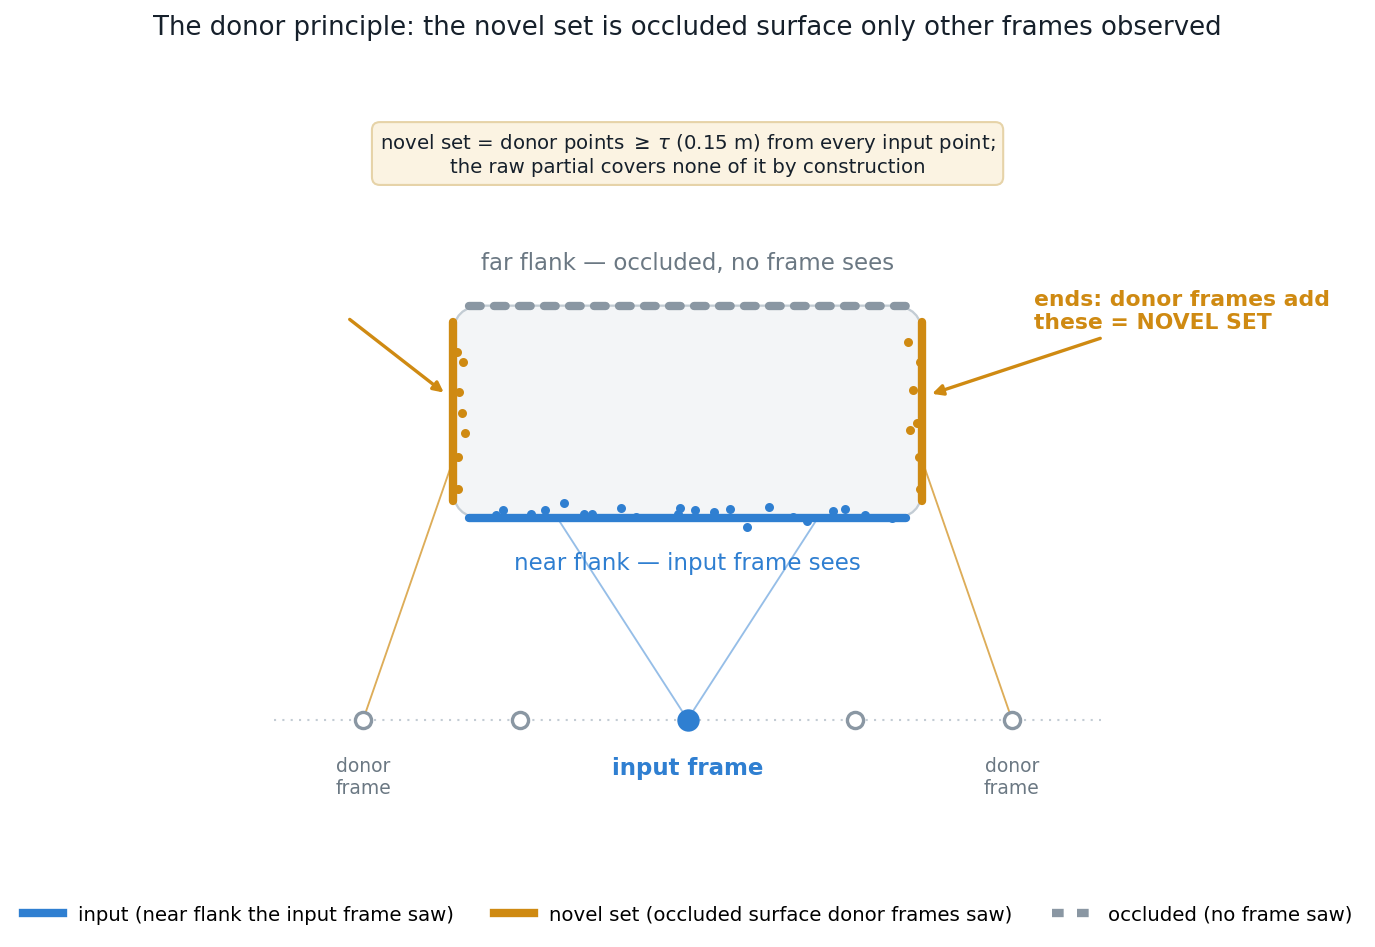
\includegraphics[width=0.86\linewidth]{donor_principle.png}
  \caption[Donor-frame occluded-side principle]{The donor-frame occluded-side principle (schematic; a car seen from
    above, the road below). The input frame observes the near flank (blue); as the
    ego drives past, the \emph{donor} frames additionally observe the two ends
    (amber), which together form the \emph{novel set} --- the surface the metric
    scores against. The far flank (grey) is occluded from every frame and is not
    part of the reference. Because the novel set lies at least $\tau$ from every
    input point, the raw partial covers none of it by construction. Illustrative
    geometry, not measured data; real per-car coverage on seq~08 is
    Figure~\ref{fig:donor-coverage}.}
  \label{fig:donor-principle}
\end{figure}

\paragraph{Relation to existing completion metrics.} Completion on real LiDAR has
been scored before without a complete target, but not against the previously-unseen
surface specifically. The KITTI completion metrics introduced with
PCN~\cite{yuan2019pcnpointcompletionnetwork} --- Fidelity, Minimal Matching Distance, and
Consistency --- reference the input, a synthetic car prior, and the model's own cross-frame
outputs respectively, so a completion that merely reproduces its input can score well on
all three. Ren et al.~\cite{ren2022selfsupervised} come closest to the construction used
here: they too accumulate each tracked vehicle across frames to form a pseudo ground truth.
The difference is what the accumulation is scored against. They compare the completed cloud
to the accumulation \emph{in full}, mixing the near surface the input already observed with
the small amount the other views add; the donor metric keeps only the novel set --- the
surface at least $\tau$ from every input point --- so already-observed surface contributes
nothing and the raw partial scores zero by construction. This is also what separates the
metric from semantic scene completion~\cite{Behley_2019_ICCV}, which scores voxel occupancy
over a whole scene rather than surface coverage of one object. The novel-set restriction,
the mirrored baseline of Section~\ref{sec:donor-definition}, and the per-band hallucination
guard of Section~\ref{sec:donor-guard-lesson} are what make the metric measure
occluded-surface recovery specifically, rather than overall resemblance to an accumulated
cloud.

\subsection{Definition of the Donor-Frame Coverage Metric}
\label{sec:donor-definition}

For each (frame, instance) true-positive pair on the well-observed static cars,
we form three point sets and score them against a common target.

\paragraph{Inputs.} The \textbf{input} is the production pipeline's cluster for
that car in that frame, completed through the production path (the KITTI-like
PCN checkpoint behind the L-shape input gate). The \textbf{donor cloud} is the
union of the instance's ground-truth (labelled-car) points from every observing
frame \emph{except} the input frame, transformed to the world frame and
voxelised at \SI{3}{\centi\meter}.

\paragraph{Novel set (the visibility mask).} From the donor cloud we keep only
points that lie at least $\tau$ from \emph{every} input point (nearest-neighbour
test). This \emph{novel set} is exactly the surface the input frame did not
observe. We use $\tau = \SI{0.15}{\meter}$ as the primary radius and
\SI{0.10}{} / \SI{0.20}{\meter} as stability checks.

\paragraph{Scored clouds.} We score three clouds against the novel set so that
completion is judged against meaningful baselines rather than in isolation:
\begin{itemize}
  \item \textbf{raw} --- the partial input (the floor: covers no novel surface
    by construction);
  \item \textbf{mirrored} --- the input unioned with its own reflection across
    the car's estimated symmetry plane (a cheap, hallucination-free way to add
    surface; the baseline completion must beat to justify a learned model);
  \item \textbf{completed} --- the PCN output.
\end{itemize}

\paragraph{Scores.} Each cloud gets three numbers, all one-directional from the
novel set to the cloud:
\begin{itemize}
  \item \textbf{coverage} (\texttt{cov@0.1}) --- the fraction of novel points
    within \SI{0.1}{\meter} of the cloud (the primary quality score: how much
    unseen surface was recovered);
  \item \textbf{median novel distance} --- the median distance from novel points
    to the cloud (a threshold-free companion to coverage);
  \item \textbf{out-of-box} --- the fraction of the cloud's points falling
    outside the amodal ground-truth box (plus a \SI{0.2}{\meter} margin): a
    \emph{hallucination guard}, since a model can trivially raise coverage by
    inventing surface everywhere.
\end{itemize}

\paragraph{Eligibility.} The metric applies to any completion whose input is a
\emph{single, well-formed object cluster} --- one cluster corresponding to one
car, with a footprint consistent with a whole vehicle --- so that there is a
coherent object shape to score. In this pipeline that admission is realised by the
L-shape input gate of Section~\ref{ch:completion-method} (fitted footprint length
$\geq \SI{2.7}{\meter}$ and width $\leq \SI{2.3}{\meter}$, rejecting fragments and
merges), but the metric itself does not depend on that particular gate: any
admission rule that isolates a single object serves in its place.

\paragraph{Statistics.} A pair counts if its input is admitted and its novel set
has at least \num{100} points at the primary $\tau$. Because the frames of one
parked car are autocorrelated, we reduce each car to its per-car median and test
across cars with the Wilcoxon signed-rank test --- the same paired, per-car design
used for the box evaluation.

\subsection{Summary and Methodological Limitations}
\label{sec:meth-limitations}

This chapter has set out the full method: the modular detection pipeline that turns a
raw scan into car detections, the single-frame completion path with its input gate and
length prior, and the definition of the donor-frame coverage metric. Several limitations
are built into these choices and are flagged here so the evaluation is read with them in
view; each is taken up in full in the discussion of Chapter~\ref{ch:conclusion}.

\begin{itemize}
  \item \textbf{Ground model.} A single global RANSAC plane assumes near-planar
    ground; it holds on the flat urban sequences used here but would degrade on
    strong slopes, where a grid-based model (future work) would be needed
    (Section~\ref{sec:pipeline-ground}).
  \item \textbf{Offline by design.} The tracker and track-level filter consult the
    whole sequence, and at $\approx$\SI{1.6}{\fps} the pipeline is far below sensor
    rate; real-time operation is out of scope (Section~\ref{sec:pipeline-overview}).
  \item \textbf{Single-frame, static-car completion.} Completion runs on one frame's
    cluster, and the donor metric is defined on static cars; moving cars are treated
    separately and are not scored for completion accuracy
    (Section~\ref{sec:completion-what}).
  \item \textbf{Length-prior fallback.} The per-car length estimate falls back to the
    fixed \SI{4.14}{\meter} prior on \SI{23}{\percent} of tracks (those with fewer
    than five gate-passed frames), and a residual far-end under-extension on long cars
    is a characterised, not eliminated, limit (Sections~\ref{sec:completion-length}
    and~\ref{sec:completion-step1c}).
  \item \textbf{Synthetic-only completion training.} PCN sees only synthetic
    KITTI-like partials; real-data fine-tuning was a negative result, so a sim-to-real
    residual remains (Section~\ref{sec:completion-domaingap}).
  \item \textbf{Metric admissibility.} The donor metric requires a single well-formed
    object cluster and multi-frame donor observations, so it does not score fragments,
    merges, or movers (Section~\ref{sec:donor-definition}).
\end{itemize}

With these caveats stated, Chapter~\ref{ch:evaluation} puts each component to the test
--- the detection operating point and its ablations, the recall root-cause, and the
donor metric's validation and completion results --- and Chapter~\ref{ch:conclusion}
returns to the limitations above alongside the evaluation-validity questions the results
raise.

               % Chapter 3: detection pipeline + object completion
% Chapter 4 -- Evaluation (\input by main.tex): detection protocol + detection results
% + recall analysis + donor-metric validation + completion results. Merged from the
% former sec_4_1 / sec_4_results / sec_5 / sec_7_2 / sec_7_results fragments (seam
% markers below).
%
% Honesty-phrasing rules applied (personal_agenda P1):
%   - "mean IoU" always qualified as "of matched detections"
%   - recall denominator stated explicitly (>=10 points surviving preprocessing)
%   - evaluation is leave-one-sequence-out (LOSO): each sequence is scored by a
%     classifier that never saw it in training or selection; seq 08 is the reported
%     operating point (fold-08 confirms the final seq-08 numbers)
%   - measured vs inferred evidence tiers marked in prose
%   - every number traceable to a finding / output artifact
%
\chapter{Evaluation}
\label{ch:evaluation}

This chapter evaluates the full pipeline end to end, but its destination is the
contribution: the donor-frame coverage metric and what it reveals about
completion. The route there runs through the detection front-end that supplies
the metric its inputs. We first fix the detection evaluation protocol
(Section~\ref{sec:eval-protocol}) and report the detection operating point,
ablations, range, and runtime (Sections~\ref{sec:results-detection}--\ref{sec:results-runtime});
we then diagnose why detection recall is capped, because the same clustering
step that limits recall is what governs input cleanliness for completion
(Section~\ref{sec:recall-analysis}). The chapter then turns to its centre: the
donor metric is put through its validation battery
(Section~\ref{sec:donor-validation}) and used to score completion on real cars ---
surface coverage, the downstream amodal box, moving cars, and a pre-registered
held-out replication (Sections~\ref{sec:results-coverage}--\ref{sec:results-heldout}).

\section{Evaluation protocol}
\label{sec:eval-protocol}

Every quantitative claim about detection in this thesis is produced by a single
evaluation script (\texttt{src/evaluate.py}) under one fixed protocol. Because
the results, ablation, and recall-analysis sections all report numbers from this
protocol, we state it in full here and refer back to it rather than restating it
per table. The protocol was frozen before the write-up began; no configuration,
checkpoint, or metric definition described below was altered to produce a
reported number.

\subsection{Sequences, roles, and leave-one-sequence-out cross-validation}
\label{sec:eval-sequences}

We evaluate on the eleven labelled SemanticKITTI odometry sequences
(\numrange{00}{10}), whose per-point semantic and instance labels serve as
ground truth. The official test sequences \numrange{11}{21} carry \emph{no}
public labels, so no ground-truth detection metric can be computed on them; this
is a property of the dataset, not a choice, and it is why no labelled sequence
can be reserved as a conventional held-out test set.

\paragraph{Classifier evaluation uses leave-one-sequence-out cross-validation.}
Rather than report detection on the sequence the classifier was tuned against, we
evaluate the binary classifier under \emph{leave-one-sequence-out} (LOSO)
cross-validation over all eleven sequences. For each held-out sequence~$K$ a
classifier is trained on the other ten sequences and then run on the full
sequence~$K$; the held-out sequence contributes \emph{zero} clusters to that
fold's training data and is never used to select the checkpoint. Checkpoint
selection is removed entirely: every fold trains for a fixed \num{15}-epoch
budget and the last-epoch checkpoint is used (historically the best epoch was
\num{13}/\num{15}, so last~$\approx$~best), so the held-out sequence is untouched
during both training and model selection. In the per-fold table below,
therefore, the classifier scoring sequence~$K$ has never seen
sequence~$K$ during training or model selection. Because the
Stage~B clusters are stored with a sequence prefix in their filenames, the folds
are a re-partition of the existing mined data and require no re-mining.

\paragraph{Two sequences carry additional, distinct roles.}
\begin{itemize}
  \item \textbf{Sequence 08 (reported operating point; \num{4071} frames).} The
    largest labelled sequence is the operating point at which the pipeline is
    reported in detail: the stage ablations (Section~\ref{sec:results-ablations}),
    the recall root-cause analysis (Section~\ref{sec:recall-analysis}), the
    IoU-threshold sensitivity below, and the completion evaluation
    (Section~\ref{sec:donor-validation}) are all computed on the sequence-08 output
    of the \emph{final} classifier. Sequence~08 was never used to tune the
    classical stages. The final classifier was historically selected on
    sequence~08, so its sequence-08 numbers could in principle be optimistic; the
    LOSO fold-08 classifier (trained on \numrange{00}{07},\,\numrange{09}{10},
    last-epoch, never selected on 08) settles this empirically below.
  \item \textbf{Sequence 00 (completion held-out; 100 frames).} Sequence~00 is
    the held-out sequence for the \emph{completion} replication
    (Section~\ref{sec:donor-validation}), where its being unseen by the completion
    model is what matters. Its classical pipeline parameters
    (\texttt{PIPELINE\_CONFIG}) were historically hand-tuned on it, so the
    seq-00 detection fold retains classical-stage familiarity even though its
    classifier is still properly held out; we isolate that residual in the
    aggregate below (dropping fold-00 moves pooled recall by \num{0.022}).
\end{itemize}

\subsection{Ground-truth targets and the eligibility rule}
\label{sec:eval-targets}

The pipeline is a car detector, so the evaluation counts only the two
car-bearing SemanticKITTI classes as valid ground-truth objects:
\emph{car} (class~10) and \emph{moving-car} (class~252); we refer to this target
set as \emph{supported-vehicles}. A ground-truth car \emph{instance} is a
maximal set of points sharing one instance id within these classes.

An instance is counted in the evaluation only if at least \textbf{10 of its
points survive preprocessing} --- the $z$-filter, voxel downsampling, statistical
denoising, and ground removal that every scan passes through before clustering.
This is the recall denominator: \emph{recall is computed against ground-truth car
instances with $\geq 10$ points surviving preprocessing}, not against every
annotated car. The rule exists because an instance reduced to a handful of points
by occlusion or range cannot be segmented by any clustering method, so including
it would measure sensor sparsity rather than the pipeline.

This choice narrows the denominator, and honesty requires quantifying by how
much. On a stride-20 sample of sequence~08 (204 of \num{4071} frames, drawn
uniformly across the drive), of all annotated car instances
(\num{2332} pooled), \textbf{25.5\% are excluded} by the surviving-points rule;
measured instead against instances that have $\geq 10$ points in the \emph{raw}
scan (\num{2033} pooled), \textbf{14.6\% are excluded} by preprocessing.\footnote{%
These are two distinct $\geq 10$-point rules: one thresholds \emph{raw} label
points (a distinct-car count), the other thresholds points \emph{surviving
preprocessing} (the eval denominator). They are not interchangeable.}
Because an excluded instance can never be matched, the sequence-08 operating-point
recall of \num{0.730} against the eligible denominator corresponds, by inference, to a
recall of \emph{approximately} \num{0.54} against \emph{all} annotated cars
(the eligible-to-annotated survival ratio on this sample is
$\num{1737}/\num{2332}=\num{0.745}$; the ratio is a stride-20 estimate, so this
figure is inferred, not separately measured). We report the eligible-denominator
recall as the headline and disclose the all-annotated figure alongside it.

\subsection{Matching and metrics}
\label{sec:eval-matching}

Detections and ground-truth instances are compared at the \emph{point level}.
For a detection mask $D$ and an instance mask $G$ over the surviving points, the
overlap is the intersection-over-union
\[
  \mathrm{IoU}(D,G) \;=\; \frac{|D \cap G|}{|D \cup G|}.
\]
All detection--instance pairs with $\mathrm{IoU} \geq \tau$ are collected, sorted
by descending IoU, and assigned \emph{greedily and one-to-one}: the highest-IoU
pair is matched first, and once a detection or an instance is used it cannot be
matched again. This yields, per frame:
\begin{itemize}
  \item a \textbf{true positive} (TP) for each matched pair,
  \item a \textbf{false positive} (FP) for each unmatched detection,
  \item a \textbf{false negative} (FN) for each unmatched eligible instance.
\end{itemize}
Precision, recall, and $F_1$ are then computed from TP, FP, and FN
\emph{micro-averaged} over the sequence: counts are pooled across all frames and
the ratios taken once, so denser frames contribute proportionally more. We also
report the \textbf{mean IoU of matched detections} --- the mean of the IoU values
of the accepted TP pairs only. This is a quality measure of the matches that were
made; it says nothing about missed cars and must not be read as an overall
segmentation score.

Track-level filtering is enabled by default for the headline numbers: an offline
centroid tracker links detections across frames, and only tracks meeting a
minimum length and class-consistency requirement are accepted. This is a
post-hoc, offline step (it uses the whole sequence), consistent with the
offline scope of the system; its effect is isolated as an ablation row in the
ablation section (Section~\ref{sec:results-ablations}).

\subsection{Operating point}
\label{sec:eval-operating-point}

Table~\ref{tab:headline} gives the reported operating point on the full
sequence~08 under this protocol, produced by the final classifier (the one the
completion pipeline actually runs with). This is the operating point the
ablation and recall-analysis sections of this chapter decompose; the
cross-validation that confirms it follows in Section~\ref{sec:eval-loso}.

\begin{table}[H]
  \centering
  \caption[Reported detection operating point]{Reported detection operating point under the frozen protocol, using
    the final classifier. Sequence~08 is the largest labelled sequence and was
    never used to tune the classical stages; sequence~00 is a completion held-out
    reference whose classifier saw seq-00 clusters in training (so its detection
    recall reads optimistically). Mean IoU is the mean over matched detections
    only. Section~\ref{sec:eval-loso} re-scores every sequence with a classifier
    that never saw it.}
  \label{tab:headline}
  \setlength{\tabcolsep}{5pt}
  \begin{tabular}{lccccc}
    \toprule
    Sequence & Precision & Recall & $F_1$ & Mean IoU & TP / FP / FN \\
    \midrule
    08 (full, \num{4071} fr.) & 0.905 & 0.730 & 0.808 & 0.912 & \num{25478} / \num{2676} / \num{9444} \\
    00 (100 fr., reference)   & 0.967 & 0.777 & 0.862 & 0.962 & \num{1296} / \num{44} / \num{371} \\
    \bottomrule
  \end{tabular}
\end{table}

The pipeline is precision-saturated and recall-limited: false positives are flat
at roughly one per frame, while recall is set by how many eligible cars the
clustering stage recovers as single objects. The remaining sections of this
chapter report the ablations that decompose this operating point, and Section~\ref{sec:recall-analysis}
root-causes the recall shortfall.

\subsection{Leave-one-sequence-out cross-validation}
\label{sec:eval-loso}

The operating point above is reported on sequence~08, which is also the sequence
the final classifier was historically selected on. To show that this selection
does not inflate the result, and to characterise the per-sequence recall spread
that a single reporting sequence cannot, we ran the LOSO protocol of
Section~\ref{sec:eval-sequences}: eleven folds, each training a classifier on ten
sequences and evaluating the full held-out eleventh, so every fold's classifier
is blind to the sequence it scores. Table~\ref{tab:loso} reports all eleven folds,
the pooled micro-average (counts summed across folds, comparable to the single
operating-point number), and the macro mean~$\pm$~standard deviation across folds.

\begin{table}[H]
  \centering
  \caption[Leave-one-sequence-out cross-validation]{Leave-one-sequence-out cross-validation over all eleven labelled
    sequences (full sequences, $\tau=0.3$, final configuration). Each fold's
    classifier trained on the other ten sequences and was never selected on the
    held-out one, so no row's classifier has seen the sequence it scores.
    ``Pooled'' sums TP/FP/FN across folds; the excl.-seq00 pool isolates the
    residual seq-00 classical-tuning familiarity (Section~\ref{sec:eval-sequences}).}
  \label{tab:loso}
  \setlength{\tabcolsep}{3pt}
  \footnotesize
  \begin{tabular}{lccccc}
    \toprule
    Held-out seq & Precision & Recall & $F_1$ & Mean IoU & TP / FP / FN \\
    \midrule
    00 (\num{4541} fr.) & 0.913 & 0.761 & 0.830 & 0.932 & \num{42763} / \num{4079} / \num{13427} \\
    01 (\num{1101} fr.) & 0.951 & 0.336 & 0.496 & 0.953 & \num{539} / \num{28} / \num{1067} \\
    02 (\num{4661} fr.) & 0.793 & 0.700 & 0.743 & 0.903 & \num{10919} / \num{2857} / \num{4685} \\
    03 (\num{801} fr.)  & 0.733 & 0.623 & 0.673 & 0.904 & \num{1527} / \num{556} / \num{926} \\
    04 (\num{271} fr.)  & 0.797 & 0.501 & 0.615 & 0.835 & \num{529} / \num{135} / \num{527} \\
    05 (\num{2761} fr.) & 0.861 & 0.731 & 0.791 & 0.910 & \num{10671} / \num{1723} / \num{3927} \\
    06 (\num{1101} fr.) & 0.861 & 0.637 & 0.732 & 0.906 & \num{6374} / \num{1031} / \num{3637} \\
    07 (\num{1101} fr.) & 0.905 & 0.729 & 0.808 & 0.929 & \num{11131} / \num{1162} / \num{4137} \\
    08 (\num{4071} fr.) & 0.881 & 0.737 & 0.803 & 0.912 & \num{25733} / \num{3477} / \num{9189} \\
    09 (\num{1591} fr.) & 0.824 & 0.646 & 0.724 & 0.911 & \num{5141} / \num{1097} / \num{2813} \\
    10 (\num{1201} fr.) & 0.725 & 0.559 & 0.632 & 0.871 & \num{1832} / \num{694} / \num{1444} \\
    \midrule
    \textbf{Pooled (all 11)} & \textbf{0.874} & \textbf{0.719} & \textbf{0.789} & \textbf{0.919} & \num{117159} / \num{16839} / \num{45779} \\
    Pooled (excl.\ seq~00)   & 0.854 & 0.697 & 0.767 & 0.911 & \num{74396} / \num{12760} / \num{32352} \\
    Macro mean $\pm$ std     & $0.840{\pm}0.070$ & $0.633{\pm}0.121$ & $0.713{\pm}0.097$ & $0.906{\pm}0.030$ & --- \\
    \bottomrule
  \end{tabular}
\end{table}

Three things follow. First, \textbf{model selection did not inflate the reported
recall}. The fold-08 classifier, blind to sequence~08, reaches recall \num{0.737} against
the sequence-08 operating point's \num{0.730} --- if anything marginally higher,
not lower --- so the recall headline is not a product of having selected the
classifier on the reporting sequence. The model-selection optimism that does
exist is confined to precision and is small: fold-08 precision is \num{0.881}
versus the final \num{0.905} (an extra \num{801} false positives across
\num{4071} frames), exactly the two-point, precision-only exposure the stage
decomposition predicts (Section~\ref{sec:disc-eval-validity}). The two
sequence-08 rows are not two separate experiments but \emph{one classifier under
two checkpoint-selection rules}: the final model and the fold-08 model share the
same architecture, the same ten training sequences (\numrange{00}{07},
\numrange{09}{10}), and the same from-scratch \num{15}-epoch regime, and differ
only in which epoch is frozen --- the final model takes the epoch that scored
best on the sequence-08 validation set, the fold-08 model takes the last epoch and
never inspects sequence~08 at all. The \num{0.730}~$\rightarrow$~\num{0.737}
(recall) and \num{0.905}~$\rightarrow$~\num{0.881} (precision) deltas therefore
isolate the effect of that selection: selecting on sequence~08 bought about two
precision points and no recall. The isolation is not perfect --- because
sequence~08 cannot serve as the fold's loss-monitoring split, the fold-08 model
trains on \SI{95}{\percent} of the final model's clusters (a \num{5}-percent
monitoring slice is set aside) --- but that confound removes training data from
the fold-08 model, which would depress its recall, not inflate it, so it only
strengthens the ``recall was not inflated'' reading. Second, the
\textbf{pooled cross-validated operating point} over all eleven sequences ---
precision \num{0.874}, recall \num{0.719}, $F_1$~\num{0.789}, mean IoU
\num{0.919} --- sits within roughly one point of the sequence-08 operating point
on every metric, so the reported numbers are representative of the labelled set
and not specific to sequence~08. Third, the \textbf{per-sequence spread} is now
explicit: recall ranges from \num{0.336} on sequence~01 (a sparse highway drive)
to \num{0.761} on sequence~00 (dense urban), with a macro mean of
\num{0.633}~$\pm$~\num{0.121}; precision is far steadier
(\num{0.840}~$\pm$~\num{0.070}). The gap between the pooled recall (\num{0.719})
and the macro mean (\num{0.633}) is driven by the smallest, sparsest sequences
(seq~01 and seq~04, the latter only \num{271} frames), which the count-weighted
pool down-weights and the unweighted mean does not; both figures are reported so
neither hides the spread. Finally, the residual seq-00 classical-tuning exposure
is bounded: dropping the seq-00 fold lowers pooled recall only from \num{0.719}
to \num{0.697} (a \num{0.022} delta), so the historical seq-00 pipeline tuning
does not drive the aggregate.

\subsection{Choice of IoU threshold and its sensitivity}
\label{sec:eval-iou-threshold}

All headline numbers use $\tau = 0.3$. A point-level threshold of 0.3 is
permissive relative to the bounding-box 0.5 common in detection benchmarks, so
it is fair to ask whether the results are an artifact of a lenient gate. They
are not, and the reason is visible in Table~\ref{tab:headline}: the mean IoU of
matched detections is \num{0.912} on sequence~08, far above either threshold, so
the matches are not marginal overlaps sitting just past $\tau$.

To make this concrete we re-ran the full sequence~08 evaluation at
$\tau \in \{0.25, 0.30, 0.50\}$ with everything else frozen
(Table~\ref{tab:iou-sensitivity}).

\begin{table}[H]
  \centering
  \caption[IoU-threshold sensitivity on seq~08]{IoU-threshold sensitivity on the full sequence~08 (frozen
    configuration). The $\tau = 0.30$ row is the headline. $F_1$ moves by at most
    \num{2.6} points across the tested range (\num{0.811} at $\tau=0.25$ to
    \num{0.785} at $\tau=0.50$); mean IoU of matched detections rises at the
    stricter gate because it keeps only the better-overlapping matches.}
  \label{tab:iou-sensitivity}
  \begin{tabular}{cccccc}
    \toprule
    $\tau$ & Precision & Recall & $F_1$ & Mean IoU & TP / FP / FN \\
    \midrule
    0.25 & 0.908 & 0.732 & 0.811 & 0.910 & \num{25576} / \num{2578} / \num{9346} \\
    0.30 & 0.905 & 0.730 & 0.808 & 0.912 & \num{25478} / \num{2676} / \num{9444} \\
    0.50 & 0.879 & 0.709 & 0.785 & 0.927 & \num{24744} / \num{3410} / \num{10178} \\
    \bottomrule
  \end{tabular}
\end{table}

$F_1$ falls only \num{2.3} points from the headline $\tau = 0.30$ to the strict
$\tau = 0.50$ (\num{0.808} to \num{0.785}), and \num{2.6} points across the full
tested range from the permissive $\tau = 0.25$ (\num{0.811}), so the reported
quality is stable under the choice of threshold and does not depend on the lenient
value. We had
pre-registered that a threshold-sensitive result would be \emph{reported as a
finding rather than tuned away}; it was not sensitive.


%% ===== merged from sec_4_results.tex ===== %%

% Detection Results, Ablations, Range, Runtime (Sections 4.2--4.5; folds under Chapter 4).
% Opens with \section{Detection Evaluation} carrying its own distinct label
% (\label{ch:detection-eval-results}), which does not clash with the chapter's
% \label{ch:evaluation}.
%
% Honesty-phrasing rules applied (personal_agenda P1):
%   - "mean IoU" always qualified as "of matched detections"
%   - recall denominator restated / cross-referenced (>=10 surviving points)
%   - seq 08 = classifier model-selection set, not a held-out test set
%   - negative results reported AS FINDINGS, not apologised for
%     (C5 synthetic-pretraining redundant; clustering "adopt nothing")
%   - the distance table is per-frame / track-filter-OFF: stated as a deviation,
%     read as a trend, NOT a restatement of the 0.730 headline
%   - every number traces to a finding / output artifact (cited Finding~\#NN)
%
\section{Detection results}
\label{sec:results-detection}

The headline operating point is the sequence~08 row of Table~\ref{tab:headline}
(Section~\ref{sec:eval-protocol}): precision \num{0.905}, recall \num{0.730}, $F_1$ \num{0.808}, and
a mean IoU of matched detections of \num{0.912}, over
\num{25478}~/~\num{2676}~/~\num{9444} TP~/~FP~/~FN. Two properties of this
operating point organise the rest of the chapter, and both are visible directly
in the per-frame record rather than only in the pooled totals.

First, the pipeline is \emph{precision-saturated}. Across the full sequence the
false-positive count is low and stable --- about \num{0.7} per frame
(\num{2676} over \num{4071} frames), independent of how many cars are in view.
Figure~\ref{fig:bev-detections} shows this spatially --- detections track the
true parked and moving cars along the street, with few spurious boxes --- and
Figure~\ref{fig:timeseries} shows it over time: the FP trace is low and
stationary while the number of ground-truth cars per frame swings widely.

Second, the pipeline is \emph{recall-limited}, and the limit is structural. The
recall shortfall traces to a measured clustering failure: HDBSCAN splits large,
close cars into fragments that no longer match a single instance, and the split rate is highest exactly where cars are densest and
nearest (\SI{66}{\percent} at \SIrange{0}{10}{\metre}).
Section~\ref{sec:results-distance} exhibits the resulting near-range recall dip
directly, and the time series (Figure~\ref{fig:timeseries}) shows per-frame
recall tending to fall in the denser frames while false positives stay flat. We
root-cause the splitting mechanism in Section~\ref{sec:recall-analysis}; here we establish only that
recall, not precision, is the dominant error mode, and that it does not come from
the classifier misfiring (false positives stay flat regardless).

\begin{figure}[htbp]
  \centering
  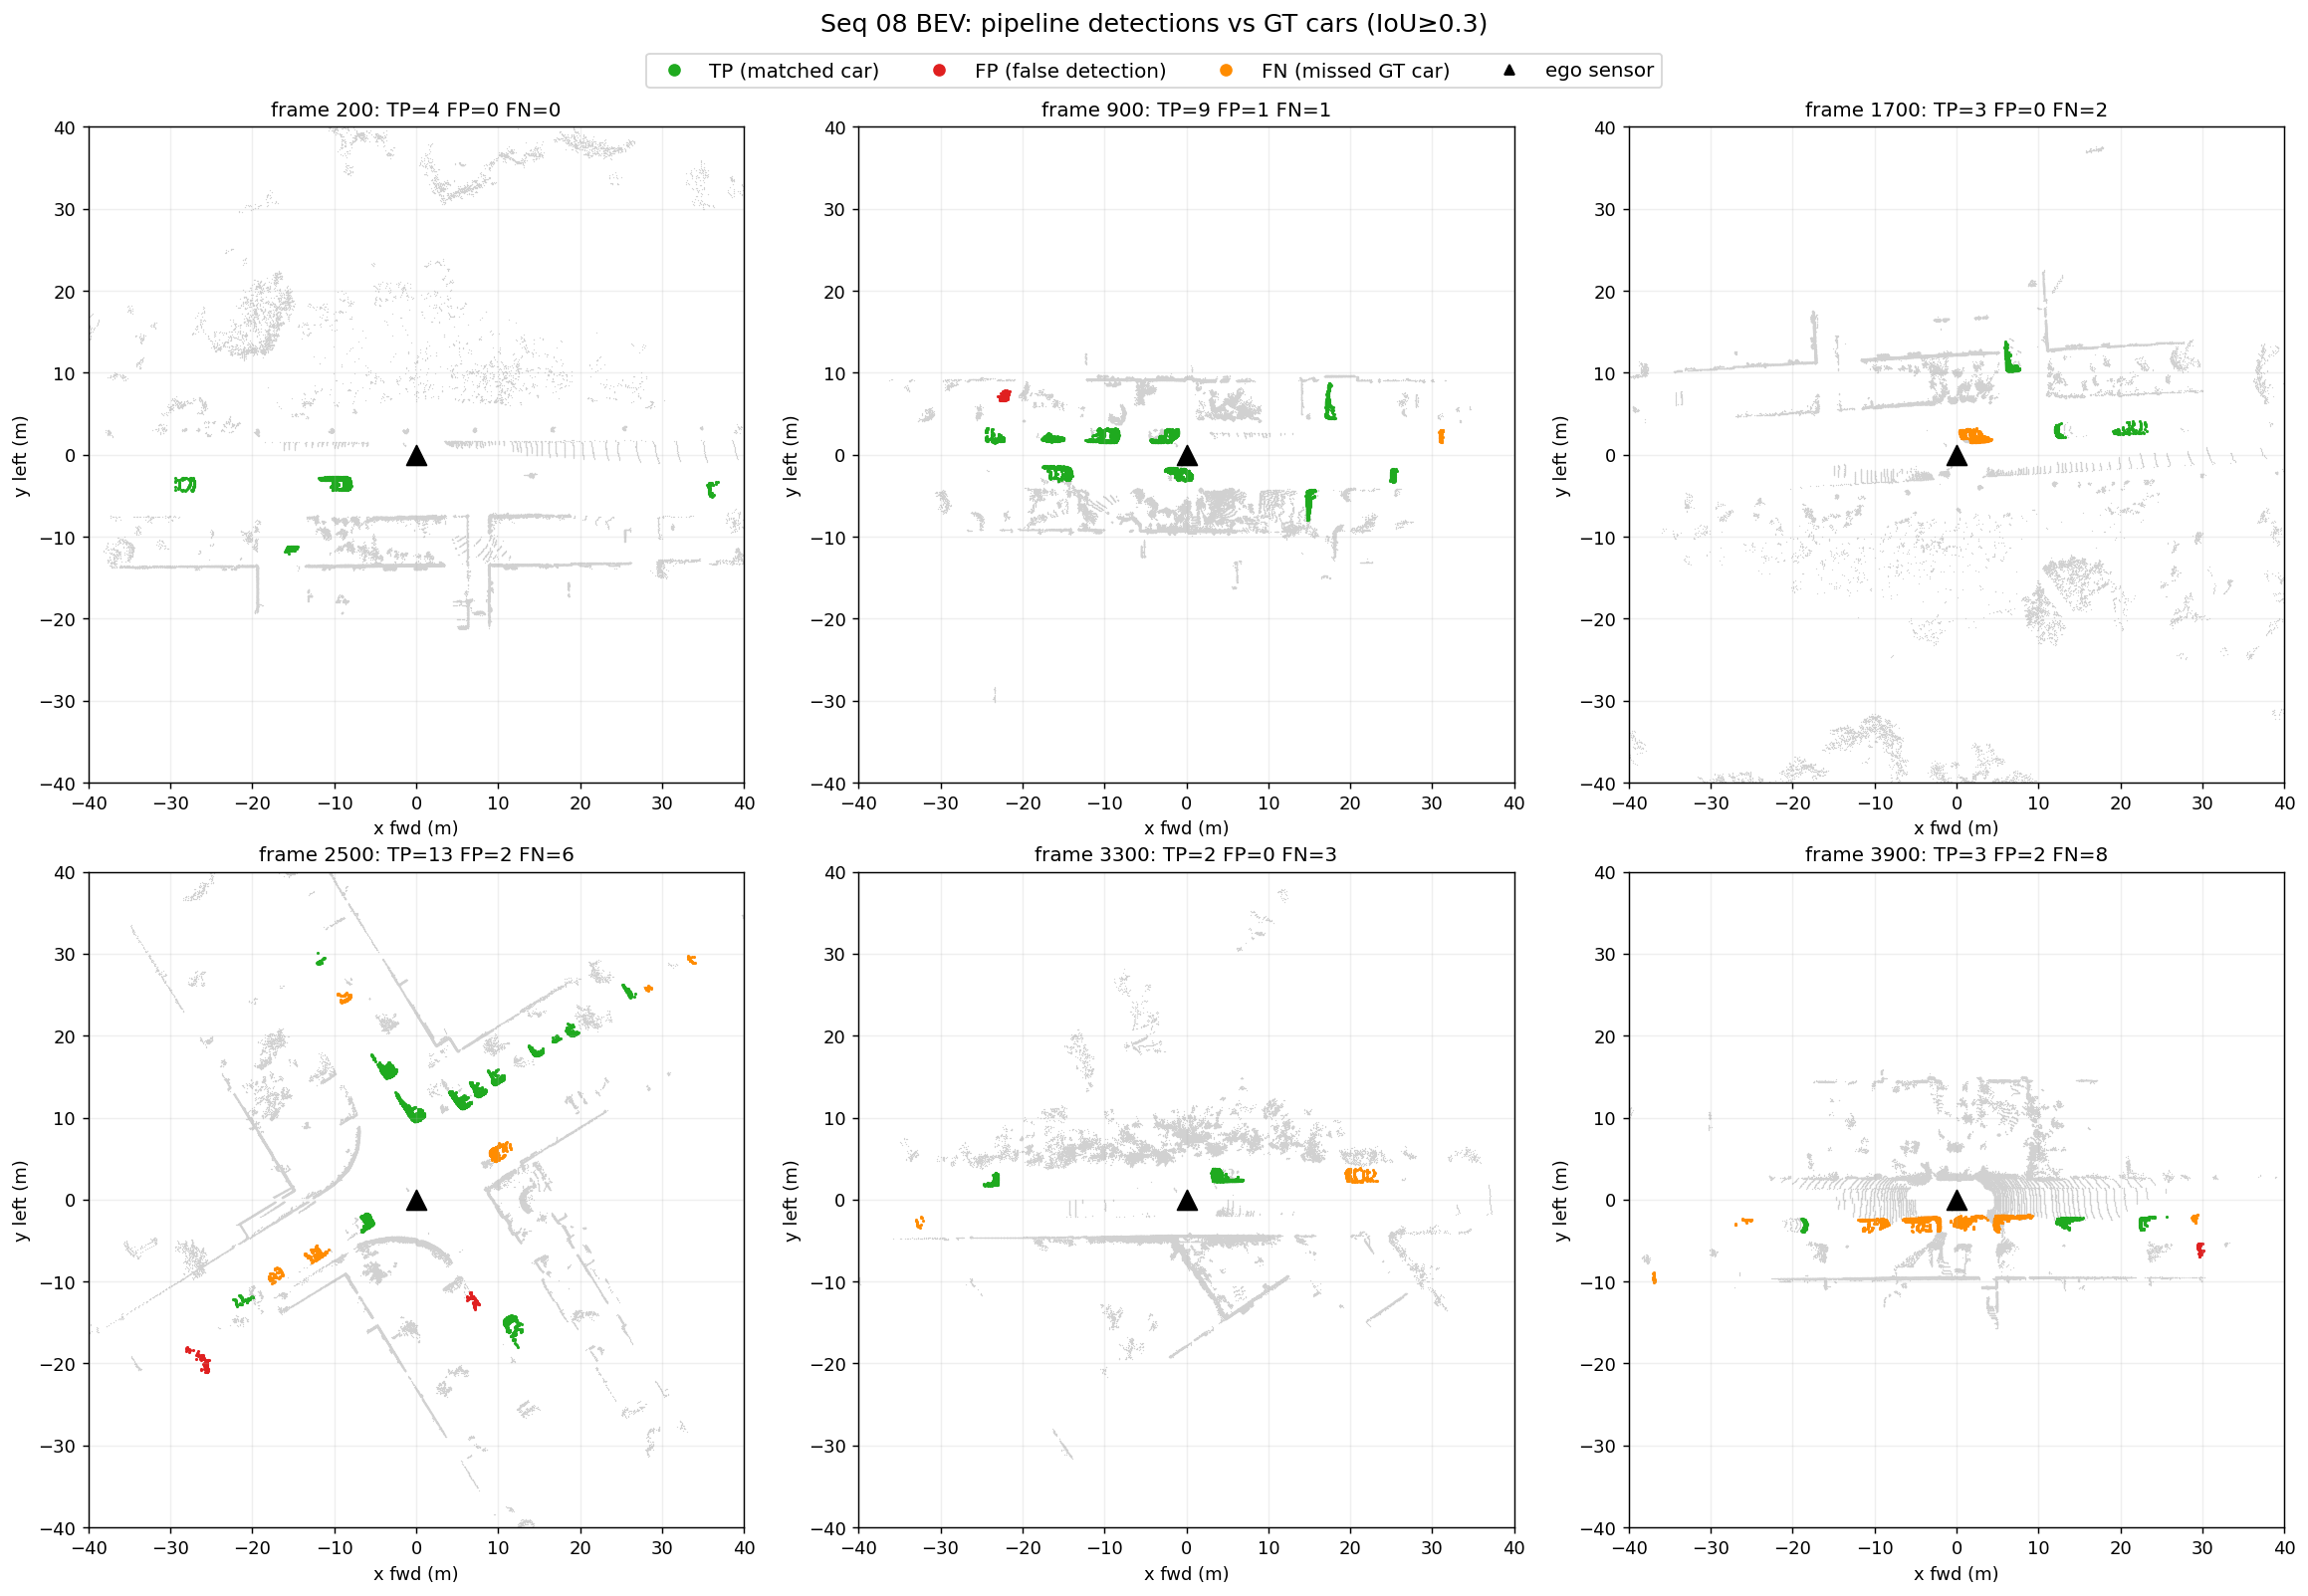
\includegraphics[width=\linewidth]{seq08_bev_detections.png}
  \caption[Bird's-eye view of detections on seq~08]{Bird's-eye view of detections on a representative sequence~08 frame.
    Detected car clusters (coloured) are overlaid on the ground-removed point
    cloud; ego is at the origin. Detections concentrate on true vehicles, with
    few spurious clusters --- the precision-saturated behaviour reported in
    Table~\ref{tab:headline}.}
  \label{fig:bev-detections}
\end{figure}

\begin{figure}[htbp]
  \centering
  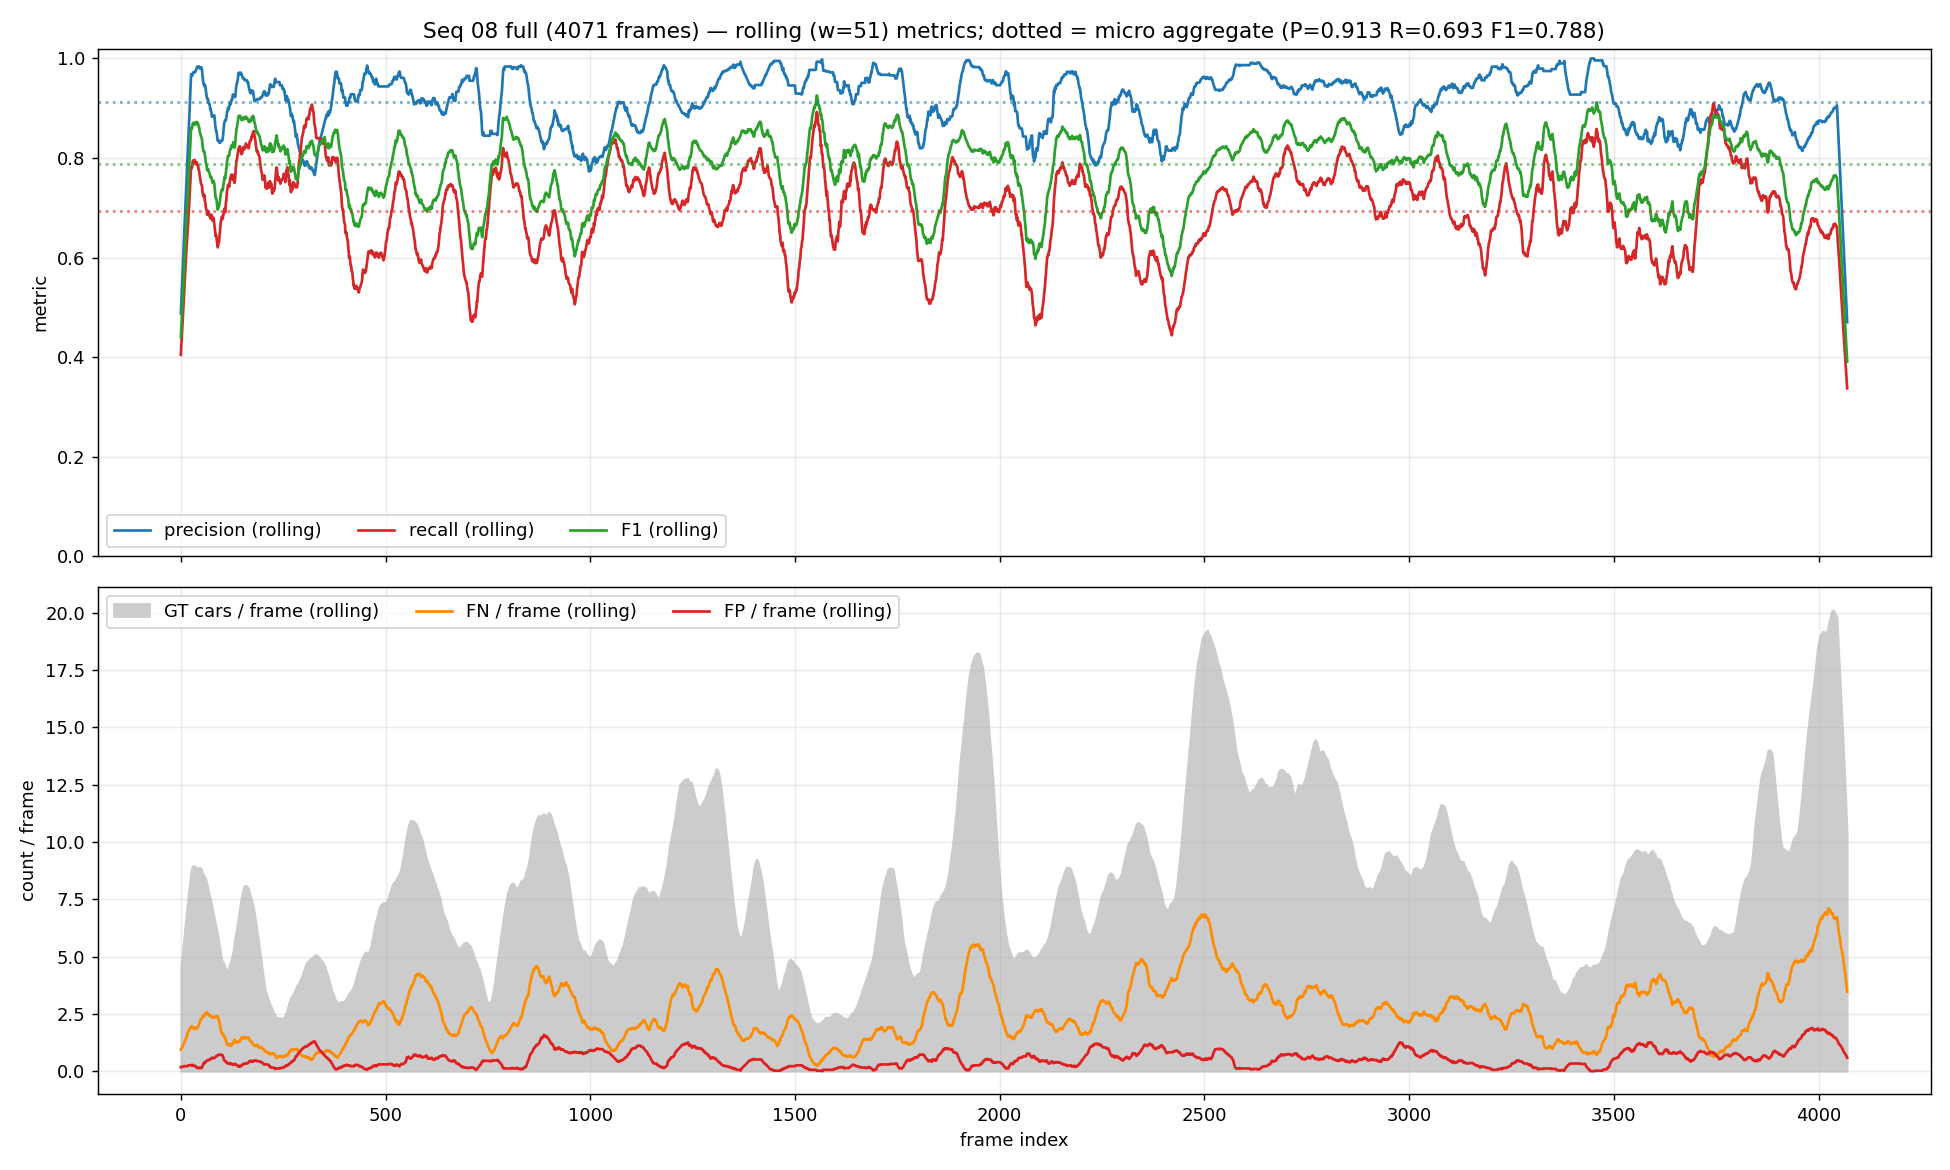
\includegraphics[width=\linewidth]{seq08_timeseries.png}
  \caption[Per-frame detection behaviour on seq~08]{Per-frame detection behaviour over sequence~08. False positives (lower
    trace) stay low and flat --- under one per frame --- regardless of scene
    content, while per-frame recall tends to fall in frames with more
    ground-truth cars. The structural recall limit is root-caused in Section~\ref{sec:recall-analysis}
    (HDBSCAN splitting).}
  \label{fig:timeseries}
\end{figure}

\section{Ablations}
\label{sec:results-ablations}

This section decomposes the headline operating point into the contribution of
each learned or post-hoc stage. Every ablation row is produced under the frozen
protocol of Section~\ref{sec:eval-protocol} unless a deviation is stated explicitly.

\subsection{Stage decomposition: classifier and track-filter contributions}
\label{sec:ablation-stage}

Table~\ref{tab:ablation-stage} isolates the two filtering stages that sit on top
of geometric clustering. The geometric-only row uses clustering plus the
geometric size/shape filters with \emph{no} learned classifier and \emph{no}
track filter (like-for-like under the promoted
configuration); the full row is the headline.

\begin{table}[H]
  \centering
  \caption[Stage ablation on seq~08]{Stage ablation on the full sequence~08 (frozen configuration). Rows
    add one filtering stage at a time on top of geometric clustering. The
    per-frame classifier is the precision mechanism (it removes $\sim$\num{149000}
    junk clusters) but is conservative on borderline cars (recall drops); the
    offline track filter then recovers recall by temporal voting while raising
    precision further. Mean IoU is over matched detections only. Geometric-only
    and the middle row are per-frame (no track filter); the full row uses the
    offline track filter.}
  \label{tab:ablation-stage}
  \setlength{\tabcolsep}{5pt}
  \begin{tabular}{lccccc}
    \toprule
    Configuration & Precision & Recall & $F_1$ & Mean IoU & TP / FP / FN \\
    \midrule
    Geometric only                & 0.149 & 0.775 & 0.250 & 0.907 & \num{27051} / \num{154612} / \num{7871} \\
    \;+\,classifier              & 0.820 & 0.677 & 0.741 & 0.921 & \num{23629} / \num{5204} / \num{11293} \\
    \;+\,classifier, track filter & 0.905 & 0.730 & 0.808 & 0.912 & \num{25478} / \num{2676} / \num{9444} \\
    \bottomrule
  \end{tabular}
\end{table}

The decomposition tells a two-step story. The \textbf{classifier
is the precision mechanism}: geometric clustering under the promoted coarse-voxel
setting emits many mostly-junk clusters (precision \num{0.149}), and the per-frame
classifier removes about \num{149000} of them across the sequence
(FP \num{154612}~$\rightarrow$~\num{5204}), lifting precision from \num{0.149} to
\num{0.820}. It pays for this with recall --- being conservative, it discards
borderline true clusters too, so recall falls from \num{0.775} to \num{0.677}.
The \textbf{track filter then recovers that recall while improving precision
again}: linking detections across frames and accepting only consistent tracks
lifts precision to \num{0.905} \emph{and} recall to \num{0.730} (TP
\num{23629}~$\rightarrow$~\num{25478}), because a car seen across many frames is
kept even where a single frame classified it as unknown, while transient
false positives fail the track-length test. The net of both stages is still a
recall trade --- geometric-only recall (\num{0.775}) exceeds the full-pipeline
recall (\num{0.730}), roughly \num{1600} true positives forgone for the
$\sim$\num{152000}-false-positive removal --- but that trade runs through a
recall dip and a partial recovery, not a simple monotone loss. We report it
rather than hiding it: the system is deliberately tuned for precision, and the
recall it forgoes here is small next to the recall it never had (Section~\ref{sec:recall-analysis}). The
pre-promotion geometric-only figure ($F_1$~\num{0.305}) is
superseded by this like-for-like \num{0.250} and kept only as a historical
record.

\subsection{Redundancy of synthetic pretraining (Stage~A ablation)}
\label{sec:ablation-stagea}

The classifier ships as a binary car/not-car network trained \emph{from scratch}
on mined real clusters (Stage~B). A natural alternative is a two-stage
recipe in which a synthetic-ShapeNet Stage~A pretraining seeds Stage~B; we tested
whether that pretraining is necessary and found it is not --- a negative result we
report as a finding, because it changes the recommended recipe.

At the classifier level, on the sequence~08 validation clusters, the from-scratch
network matches the pretrained one: macro $F_1$ \num{0.9285} from scratch versus
\num{0.9225} pretrained (the two are within run-to-run noise, with
scratch marginally ahead). At the pipeline level a small precision edge for the
pretrained checkpoint appeared on a 100-frame sample (FP \num{27} versus
\num{62}), but it was uncontrolled (different training seed and code) and
\textbf{did not survive at full scale}: on the full sequence~08 the two
checkpoints are identical in $F_1$ to three decimals. We therefore
drop Stage~A from the production pipeline and keep it as ablation material.

The reason the synthetic prior is redundant --- and cannot simply be added for
safety --- is a total, symmetric domain gap between synthetic and real point
clusters. Table~\ref{tab:cross-domain} gives the cross-domain
transfer matrix: a model trained on one domain and evaluated on the other scores
a car-class $F_1$ of \num{0.000} in \emph{both} off-diagonal directions, and
fine-tuning on real data erases whatever the synthetic pretraining had learned.
Given \num{420000} real training clusters, the real data does essentially all the
work; the synthetic prior neither helps nor, once fine-tuned, survives.

\begin{table}[H]
  \centering
  \caption[Cross-domain classifier transfer]{Cross-domain classifier transfer (car-class $F_1$). Each
    model is trained on one domain and evaluated on the other's validation set;
    diagonal cells (italic) are in-domain, for scale. Both off-diagonal cells
    collapse to \num{0.000} --- against strong in-domain performance
    (\num{0.999}, \num{0.885}) --- so synthetic and real clusters are mutually
    out-of-distribution and synthetic pretraining transfers nothing to real
    inference.}
  \label{tab:cross-domain}
  \begin{tabular}{lcc}
    \toprule
    & \multicolumn{2}{c}{Evaluated on} \\
    \cmidrule(lr){2-3}
    Trained on & Synthetic & Real \\
    \midrule
    Synthetic (Stage~A) & \emph{0.999} & 0.000 \\
    Real (Stage~B)      & 0.000        & \emph{0.885} \\
    \bottomrule
  \end{tabular}
\end{table}

\subsection{Clustering method: cost and benefit of HDBSCAN}
\label{sec:ablation-clustering}

The clustering stage is HDBSCAN. Because it is by far the most expensive stage
(Section~\ref{sec:results-runtime}), we benchmarked it against two cheaper
density/connectivity clusterers --- DBSCAN and Euclidean-tolerance clustering ---
at the same voxel resolution and under an identical pipeline
(Table~\ref{tab:clustering}). \textbf{Deviation:} this benchmark is
per-frame with the track filter \emph{off}, because it strides across the
sequence and the tracker requires contiguous frames; the numbers are therefore
comparable to each other but not to the track-filtered headline.

\begin{table}[H]
  \centering
  \caption[Clustering-method benchmark]{Clustering-method benchmark at fixed voxel resolution
    ($\SI{0.10}{\metre}$), identical pipeline, per-frame / track-filter-off. HDBSCAN wins $F_1$ on both sequences, entirely through
    recall; precision is essentially method-independent. The alternatives are
    5--7$\times$ faster. Mean IoU is over matched detections; the timing column is
    the mean per-frame clustering time.}
  \label{tab:clustering}
  \begin{tabular}{llccccc}
    \toprule
    Seq & Method & Precision & Recall & $F_1$ & Mean IoU & Clustering (mean ms) \\
    \midrule
    \multirow{3}{*}{00}
      & HDBSCAN   & 0.962 & \textbf{0.731} & \textbf{0.831} & 0.968 & 391 \\
      & DBSCAN    & 0.962 & 0.637 & 0.767 & 0.964 & 59 \\
      & Euclidean & 0.967 & 0.636 & 0.768 & 0.982 & 78 \\
    \midrule
    \multirow{3}{*}{08}
      & HDBSCAN   & 0.813 & \textbf{0.671} & \textbf{0.735} & 0.923 & 451 \\
      & DBSCAN    & 0.848 & 0.565 & 0.678 & 0.927 & 69 \\
      & Euclidean & 0.838 & 0.576 & 0.683 & 0.950 & 93 \\
    \bottomrule
  \end{tabular}
\end{table}

The gap is entirely a recall gap --- precision is within \num{0.035} across all
methods on either sequence, while HDBSCAN's recall exceeds the alternatives by
\numrange{9}{11} points. An $\varepsilon$-sweep confirms no fixed radius closes
it: the best fixed-radius setting (Euclidean at $\varepsilon=\SI{0.4}{\metre}$)
reaches $F_1$ \num{0.800} on sequence~00, still short of HDBSCAN's \num{0.831}.
HDBSCAN's variable-density criterion recovers cars that a single radius cannot,
which is exactly the recall margin that matters here. We therefore
\textbf{adopt nothing} from the benchmark and keep HDBSCAN in production, paying
its runtime cost knowingly; DBSCAN and Euclidean remain available as
command-line options for reproduction.

\section{Detection range}
\label{sec:results-distance}

Recall is not uniform in range, and the way it varies is not the naive
``far~=~worse'' monotone one might expect. Table~\ref{tab:distance} stratifies
detection by the range of each cluster's centroid from the ego sensor, on a
stride-20 sample of sequence~08 under the frozen configuration.
\textbf{Deviation:} like the clustering benchmark, this table is
\emph{per-frame with the track filter off} (striding breaks the tracker), so its
pooled recall (\num{0.671}) is a per-frame figure and does \emph{not} restate the
track-filtered headline \num{0.730}; read the table as a range \emph{trend}, not
as a re-derivation of the headline.

\begin{table}[H]
  \centering
  \caption[Detection stratified by range-to-ego on seq~08]{Detection stratified by range-to-ego on sequence~08 (stride-20 sample,
    frozen configuration, per-frame / track-filter-off). Recall is
    \emph{non-monotonic}: it dips in the nearest bin, peaks at
    \SIrange{10}{20}{\metre}, then falls with range. The nearest-bin dip is
    over-segmentation, the far decline is sparsity. Mean IoU is
    over matched detections. Summing the two near bins recovers the
    \SIrange{0}{20}{\metre} figure ($R=\num{0.829}$) comparable to the earlier
    range analysis.}
  \label{tab:distance}
  \begin{tabular}{lccccc}
    \toprule
    Range (m) & Precision & Recall & $F_1$ & Mean IoU (matched) & TP / FP / FN \\
    \midrule
    0--10   & 0.896 & 0.787 & 0.838 & 0.902 & \num{311} / \num{36}  / \num{84}  \\
    10--20  & 0.855 & \textbf{0.862} & 0.859 & 0.926 & \num{432} / \num{73}  / \num{69}  \\
    20--40  & 0.762 & 0.549 & 0.638 & 0.934 & \num{400} / \num{125} / \num{329} \\
    40+     & 0.393 & 0.196 & 0.262 & 0.943 & \num{22}  / \num{34}  / \num{90}  \\
    \midrule
    Pooled  & 0.813 & 0.671 & 0.735 & 0.923 & \num{1165} / \num{268} / \num{572} \\
    \bottomrule
  \end{tabular}
\end{table}

The counter-intuitive result is the \textbf{nearest-bin recall dip}: recall at
\SIrange{0}{10}{\metre} (\num{0.787}) is \emph{lower} than at
\SIrange{10}{20}{\metre} (\num{0.862}), even though near cars carry far more
points. This is not sparsity --- it is over-segmentation. The split-rate analysis shows
that HDBSCAN splits the majority of the very-near cars (a split rate of
\SI{66}{\percent} at \SIrange{0}{10}{\metre}, falling to \SI{4}{\percent} at
\SIrange{30}{50}{\metre}): a large, close car dissolves into several clusters,
none of which matches the whole instance, so it is counted as a miss. The nearest bin
also has the \emph{lowest} mean IoU of matched detections (\num{0.902}),
consistent with fragments eroding the overlap even on the cars that do match. We
develop this splitting mechanism, and why post-hoc fragment-merging fails to
recover it, in Section~\ref{sec:recall-analysis}.

Beyond the peak the decline is ordinary sparsity: recall falls from \num{0.862}
at \SIrange{10}{20}{\metre} to \num{0.549} at \SIrange{20}{40}{\metre} and
\num{0.196} past \SI{40}{\metre}, as cars thin to too few surviving points to
cluster or to clear the \num{10}-point eligibility rule (Section~\ref{sec:eval-protocol}).
Mean IoU of matched detections \emph{rises} with range
(\num{0.902}~$\rightarrow$~\num{0.943}): the far cars that are detected at all are
compact, single-cluster instances, so their overlap is clean even as their number
collapses. The earlier precision-only, seq-00, pre-promotion range analysis is superseded by this on-frozen-config sequence-08 table and is
retained only as a historical note.

\section{Runtime}
\label{sec:results-runtime}

Table~\ref{tab:runtime} breaks the per-frame cost down by stage, measured over
the full sequence~08 under the final (promoted) configuration
(\num{4068} timed frames, RTX~3070~Ti / Ryzen~7~7800X3D;
per-stage figures from \texttt{timing\_seq08\_full\_n4068\_combined.json}). The breakdown shows where
the time goes: the two classical geometric stages --- ground-plane RANSAC and,
above all, HDBSCAN clustering --- dominate, together taking roughly
\SI{68}{\percent} of the frame; adding preprocessing and the geometric filter,
the classical CPU stages account for about \SI{94}{\percent}, leaving the single
learned component --- the classifier --- at only $\sim$\SI{5.4}{\percent} (the
centroid/Hungarian tracker is a classical assignment step, not learned). The
classifier is \SI{33.7}{\milli\second} for the $\sim$\num{45} clusters in a frame
($\sim$\SI{0.75}{\milli\second} each) and the tracker is negligible.

\begin{table}[H]
  \centering
  \caption[Per-frame runtime by stage on seq~08]{Per-frame runtime by stage on the full sequence~08 under the final
    (promoted) configuration (\num{4068} timed frames; mean ms).
    Clustering alone is nearly \SI{60}{\percent} of the frame. The total is
    $\approx\SI{623.5}{\milli\second}$ ($\approx$\num{1.6}~fps) on this full run;
    a stride-20 sample of the same configuration estimates
    $\approx\SI{650.6}{\milli\second}$ (the two agree to within the sampling
    variation of the expensive stages). The pre-optimisation configuration
    totalled \SI{921.3}{\milli\second}. Percentages are of the
    \SI{623.5}{\milli\second} total.}
  \label{tab:runtime}
  \begin{tabular}{lcc}
    \toprule
    Stage & Mean (ms) & Share \\
    \midrule
    Data load                       & 0.7   & 0.1\% \\
    Preprocessing (z-filter, denoise, voxel) & 125.9 & 20.2\% \\
    Ground removal (RANSAC)         & 56.2  & 9.0\% \\
    Clustering (HDBSCAN)            & 370.4 & 59.4\% \\
    Geometric filter                & 36.2  & 5.8\% \\
    Classification                  & 33.7  & 5.4\% \\
    Tracking                        & 0.3   & 0.1\% \\
    \midrule
    Total                           & 623.5 & 100\% ($\approx$1.6 fps) \\
    \bottomrule
  \end{tabular}
\end{table}

The promoted configuration is itself the product of a runtime optimisation that
targeted the dominant classical stages directly: reducing the
RANSAC iteration count and coarsening the clustering voxel to \SI{0.10}{\metre}
cut the per-frame total by roughly a third, from a pre-optimisation
\SI{921.3}{\milli\second} to \SI{623.5}{\milli\second} on the full sequence
(\SI{650.6}{\milli\second} on the stride-20 sample), and the coarser voxel also
\emph{improved} detection --- it is the promoted configuration used throughout
this chapter. A sub-\SI{400}{\milli\second} target was shown to be unreachable
through the authorised optimisation tiers --- the post-ground object cloud is
intrinsically sparse, so coarser voxelisation compresses it little and the Python
HDBSCAN retains a floor of $\sim$\SI{185}{\milli\second} --- and the achieved
operating point was accepted, real-time operation being out of scope (user
decision, \num{2026}-07-23). Point-completion, when it runs, adds
$\sim$\SI{13}{\milli\second} per completed car on top of detection and is not part
of the detection budget above.


%% ===== merged from sec_5_recall_bottleneck.tex ===== %%

% The Recall Bottleneck (folds under Chapter 4 as a section, not a chapter of its own).
% Root-causes the recall shortfall established earlier in the chapter and reports the
% failed repair strategies as a negative-results contribution. Sub-tables are
% referenced by section + Finding number rather than hard-coded table number, to stay
% robust to renumbering.
%
% Honesty-phrasing rules applied (personal_agenda P1):
%   - recall denominator restated / cross-referenced (>=10 surviving points, Sec 4.1)
%   - "mean IoU" always qualified as "of matched detections"
%   - negative results (#21/#24, temporal aggregation) reported AS FINDINGS, not
%     apologised for
%   - the retracted "~0.74 hard limit" is corrected explicitly (#24 Correction / #34)
%   - two measurement eras kept separate: the pre-promotion seq-00 repair search
%     (baseline F1 0.844; #21/#24/temporal) vs the promoted-config seq-08 fix (#34)
%   - every number traces to a finding / session log artifact (cited Finding~\#NN /
%     session_history.md)
%
\section{Recall analysis: the bridge to completion}
\label{sec:recall-analysis}

The detection operating point above established two facts: the pipeline is
precision-saturated (false positives are low and flat, about \num{0.7} per frame),
and it is recall-limited, missing roughly one car in four
($R=\num{0.730}$ on sequence~08). This section explains \emph{why} the recall is
limited, and it is the bridge to the completion evaluation that follows: the same
clustering step that caps recall is the one that decides whether a detected car
reaches completion as a clean single-object cluster. We show that the shortfall is
a clustering failure rather than a classification failure
(Section~\ref{sec:recall-diagnosis}), root-cause it to HDBSCAN splitting large,
close cars into fragments (Section~\ref{sec:split-analysis}), report a search of
repair strategies that all fail to generalise (Section~\ref{sec:repairs}), and
describe the one intervention that did help --- coarsening the clustering
resolution --- which forces a correction of an earlier, overstated ``hard
ceiling'' claim (Section~\ref{sec:resolution-fix}). The negative results are
reported as findings, not apologised for: mapping which repairs fail, and why, is
itself a finding worth reporting, and it is what justifies the residual limitation carried to
Chapter~\ref{ch:conclusion}. Unless stated otherwise, the recall denominator
throughout is the one defined in Section~\ref{sec:eval-protocol} --- ground-truth
car instances with at least \num{10} points surviving preprocessing.

\subsection{The shortfall as a clustering failure}
\label{sec:recall-diagnosis}

The recall ceiling is upstream of the learned classifier. The stage decomposition
of Section~\ref{sec:results-ablations} makes this direct: geometric clustering with the
size/shape filters but \emph{no} learned classifier and \emph{no} track filter
already reaches recall \num{0.775}, which is \emph{higher} than the full pipeline's
\num{0.730}. Every learned stage that follows can only hold or reduce that recall:
the classifier discards clusters, and the centroid tracker only re-labels and
filters clusters that geometric clustering has already produced --- it emits a
detection in a frame only where a cluster exists in that frame, and never
interpolates a detection across a gap (\texttt{src/tracker.py};
\texttt{src/evaluate.py}), so neither stage can invent a detection where clustering
found nothing. Across the full sequence the two stages together trade roughly
\num{1600} true positives (\num{27051} geometric-only versus \num{25478} full) for the removal of $\sim$\num{152000} false positives; this is a
distinct trade from the $+\num{1655}$ true positives that the resolution change of
Section~\ref{sec:resolution-fix} later recovers. Whatever caps recall is therefore
already present in the clusters that geometric clustering produces, before the
classifier sees them.

The geometric filters are not the cap either. Table-level ablation of the
size/shape gates (sequence~00, \num{100} frames) shows that of the
\num{16454} HDBSCAN clusters in the sample, only \num{2651} (\SI{16.1}{\percent})
pass the filters, and \num{1827} of the rejected clusters do overlap a ground-truth
car --- dominated by \texttt{min\_volume} (\SI{67.9}{\percent} of the GT-matching
rejections) and \texttt{min\_points} (\SI{26.4}{\percent}); sequence~08 shows the
same pattern (\SI{66.5}{\percent} / \SI{28.0}{\percent}). The dominant gates are
\texttt{min\_volume} and \texttt{min\_points} --- the two that reject \emph{small}
clusters. This is consistent with the rejected clusters being the smaller
sub-fragments of cars that HDBSCAN has already split (the dominant fragment passing
while the splinters fail the size gates), which the split analysis of
Section~\ref{sec:split-analysis} then confirms is the prevailing failure mode. We
state this as an inference rather than a direct measurement: the ablation records
only that a rejected cluster overlaps \emph{some} ground-truth car
(\texttt{src/analyze\_clustering.py}), not whether that same car also retains a
surviving cluster, so it establishes that the rejections are dominated by small
fragments, not that every one belongs to an otherwise-detected car. Either way the
diagnosis points one stage further upstream, at the clustering itself.

\subsection{Root cause: HDBSCAN fragmentation of large, close cars}
\label{sec:split-analysis}

To quantify how clustering caps recall we measured, for every eligible ground-truth
car, how its points distribute across HDBSCAN clusters. Each car is
assigned to exactly one of four states that partition the population: \emph{ok} (one
dominant cluster, under \SI{30}{\percent} noise), \emph{split} (points spread over
two or more clusters), \emph{noisy} (one cluster but at or above \SI{30}{\percent}
noise), or \emph{all-noise}. A separate, cross-cutting flag marks \emph{merged} cars
(a car whose dominant cluster is shared with another car); a merged car still has a
dominant cluster, so it is \emph{not} a fifth partition class and is reported below
as a memo count rather than a table row that would be summed.
Table~\ref{tab:split} gives the result on both sequences.

\begin{table}[H]
  \centering
  \caption[Ground-truth cars across HDBSCAN clusters]{Distribution of ground-truth cars across HDBSCAN clusters
    (pre-promotion configuration; sequence~00, \num{100} frames;
    sequence~08, held-out sample). The four states partition the population and sum
    to the denominator; \emph{split} is the dominant failure mode and \emph{merging}
    (the cross-cutting memo row, not summed) is negligible. Split cars are uneven ---
    the largest fragment holds a median \num{0.92} of the points on sequence~00 and
    \num{0.77} on sequence~08 --- but a large point-fraction does not guarantee a
    match (see text): recall shows most split cars are lost.}
  \label{tab:split}
  \begin{tabular}{lcccc}
    \toprule
    & \multicolumn{2}{c}{Seq 00 (\num{1631} cars)} & \multicolumn{2}{c}{Seq 08 (\num{811} cars)} \\
    \cmidrule(lr){2-3}\cmidrule(lr){4-5}
    Status & Count & \% & Count & \% \\
    \midrule
    ok (single dominant cluster) & 1117 & 68.5 & 509 & 62.8 \\
    split (2+ clusters)          & 514  & 31.5 & 301 & 37.1 \\
    noisy / all-noise            & 0    & 0.0  & 1   & 0.1  \\
    \midrule
    partition total              & 1631 & 100  & 811 & 100  \\
    \addlinespace
    \textit{merged} (cross-cutting) & 8 & 0.5 & 0 & 0.0 \\
    \bottomrule
  \end{tabular}
\end{table}

Three things follow. First, \textbf{splitting, not merging, is the failure mode}:
\SIrange{31}{37}{\percent} of cars split, while merging is at most
\SI{0.5}{\percent}. The pipeline almost never fuses two cars into one detection; it
repeatedly breaks one car into several. Second, \textbf{the split is worst where
cars are largest and nearest}: the split rate falls monotonically with range ---
\SI{66}{\percent} at \SIrange{0}{10}{\metre}, \SI{40}{\percent} at
\SIrange{10}{20}{\metre}, \SI{19}{\percent} at \SIrange{20}{30}{\metre}, and
\SI{4}{\percent} at \SIrange{30}{50}{\metre}. Large, close cars return many points, and
HDBSCAN finds internal density variations within that dense return --- the roof line
against the body, the near side against the far side --- and cuts the car along
them. This is the mechanism behind the counter-intuitive near-range recall dip
reported in Section~\ref{sec:results-distance}: the nearest bin has \emph{lower} recall than
the \SIrange{10}{20}{\metre} bin despite carrying far more points, because a close
car dissolves into fragments that no longer match the whole instance. Third,
\textbf{the cleanly-clustered fraction tracks recall, and splitting usually loses
the car}. The fraction of cars that form one dominant cluster
(\SI{68.5}{\percent} on sequence~00, \SI{62.8}{\percent} on sequence~08) sits just
\emph{below} the recall the pipeline achieves on the same configuration
(\num{0.739} and \num{0.699} respectively). Two things follow. The pipeline recovers
essentially every cleanly-clustered car, so that fraction is close to a floor on
recall --- not a ceiling; recall exceeds it only by the few split cars whose dominant
fragment happens to survive matching and filtering. And because recall
(\num{0.699}) barely exceeds the clean fraction (\SI{62.8}{\percent}) while
\SI{37.1}{\percent} of cars split, the great majority of split cars are \emph{not}
recovered: a large dominant point-fraction (median \num{0.77}--\num{0.92}) does not
translate into a match, because matching depends on spatial overlap and on the
fragment clearing the size filters, not on point count. Splitting is therefore the
mechanism by which cars are lost, which is exactly why it is the recall bottleneck.
This also predicts the resolution fix of Section~\ref{sec:resolution-fix}: coarsening
the voxel converts split cars into clean ones, which should lift recall by shrinking
the reliance on recovering splits --- and it does, narrowing the sequence-08 gap
between the clean fraction and recall from \num{7.1} points (\SI{62.8}{\percent}
versus \num{0.699}) to \num{3.1} points (\SI{69.9}{\percent} versus \num{0.730}).

Figure~\ref{fig:failure-zooms} shows the mechanism directly on three sequence~08
frames. Missed cars (orange) appear as broken rows of points close to the ego
vehicle, each row too small on its own to survive the size filters, while cleaner
mid- and far-range cars (green) are detected as single clusters.

\begin{figure}[htbp]
  \centering
  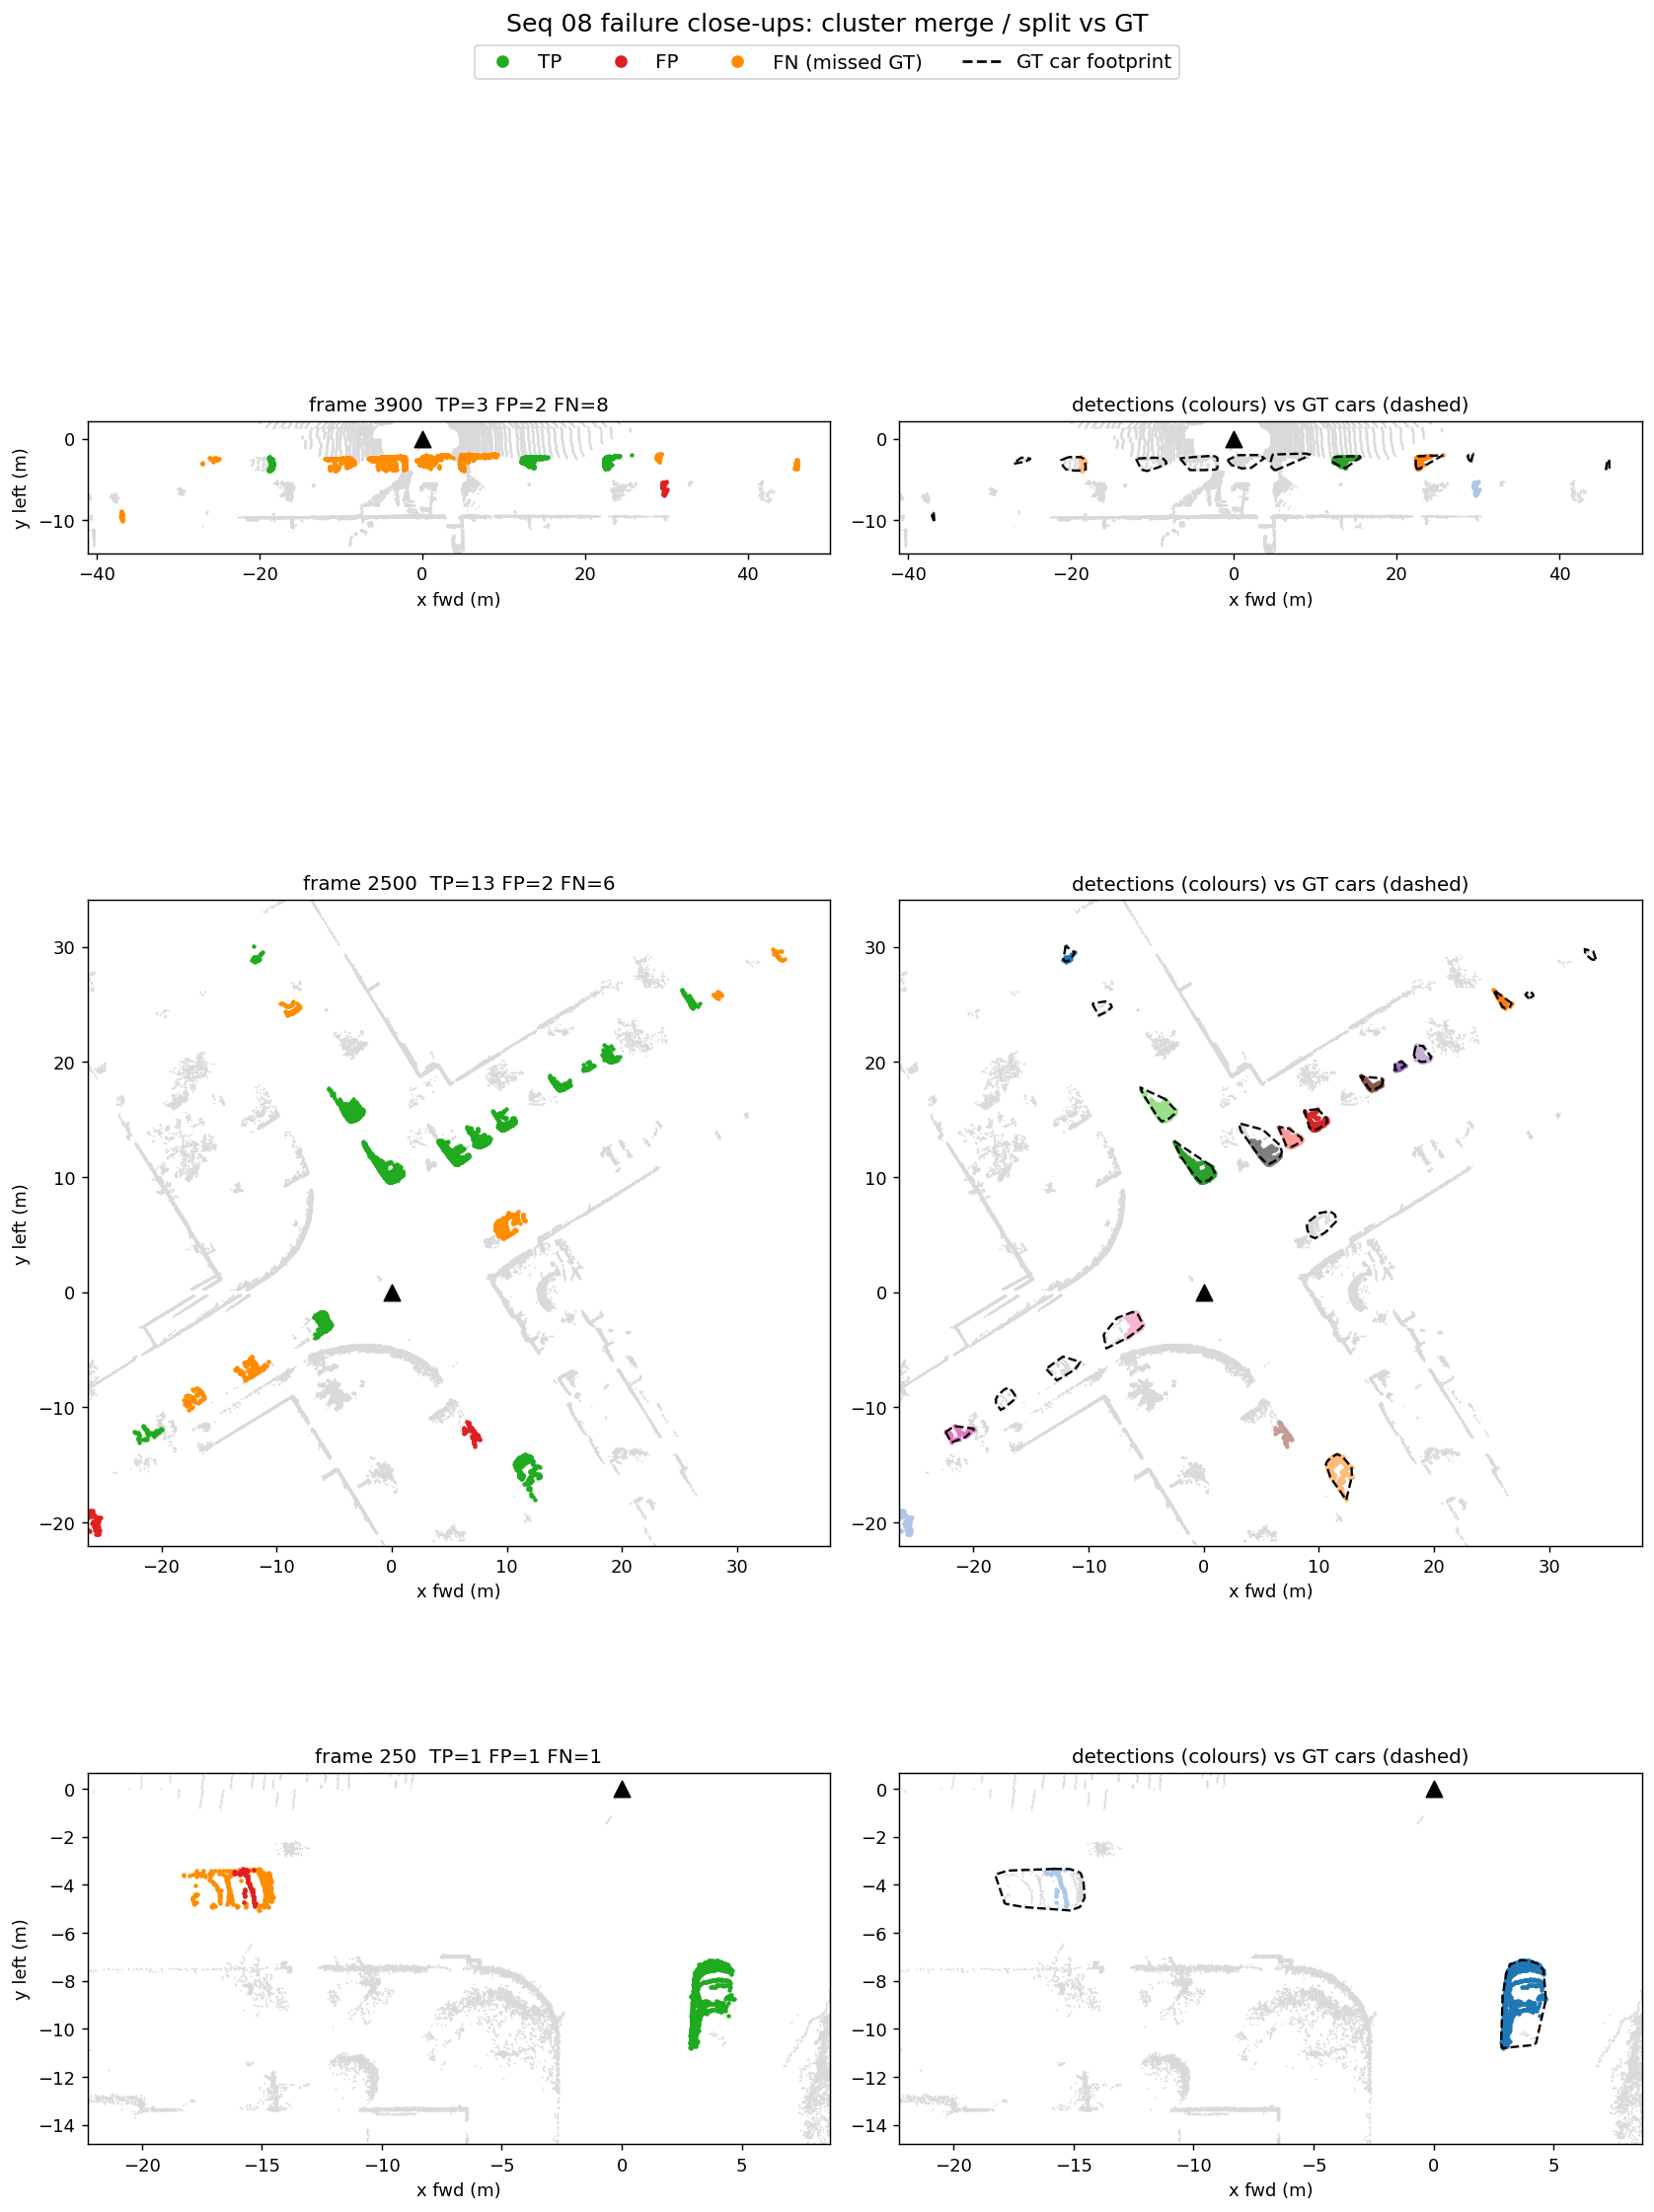
\includegraphics[width=\linewidth]{seq08_failure_zooms.png}
  \caption[Detection failure close-ups on seq~08]{Failure close-ups on sequence~08 (true positives green, false positives
    red, missed ground-truth cars orange; dashed outlines are ground-truth car
    footprints). Near-ego missed cars are fragmented into several small point groups
    rather than one cluster, matching the split mechanism of
    Table~\ref{tab:split}. Although the panel title mentions both merge and split,
    merging is measured at $\leq\!\SI{0.5}{\percent}$ (Table~\ref{tab:split}), so the
    misses shown are fragmentation, not fusion of neighbouring cars.}
  \label{fig:failure-zooms}
\end{figure}

\subsection{Limits of the repair strategies}
\label{sec:repairs}

Given that splitting caps recall, the obvious responses fall into two families:
change how clusters \emph{form} (a larger minimum cluster size, a different
clusterer, distance-adaptive parameters, or pre-clustering point accumulation) or
\emph{reassemble} fragments after HDBSCAN has split them. We tried six in total;
Table~\ref{tab:strategies} collects the four with a reproducible quantitative
outcome, and two further strategies (temporal accumulation and threshold lowering)
are discussed in prose below. All were evaluated against the same pre-promotion
sequence-00 baseline (full pipeline, classifier and track filter on;
$F_1=\num{0.844}$), and the load-bearing ones were re-checked on the held-out
sequence~08.

\begin{table}[H]
  \centering
  \caption[Recall-repair strategies]{Recall-repair strategies against the pre-promotion baseline (full
    pipeline, sequence~00, \num{100} frames; held-out sequence-08 $F_1$ where
    measured). Every strategy either loses $F_1$ outright or fails to hold its
    sequence-00 gain on the held-out sequence. This is the \emph{pre-promotion}
    repair search --- it predates the coarse-voxel configuration of
    Section~\ref{sec:resolution-fix}, which is why the baseline here is
    $F_1=\num{0.844}$, not the promoted headline. Sources in the ``Src'' column are
    finding numbers. Two further strategies --- temporal point accumulation and
    lowering the size thresholds --- are discussed in the text but omitted here:
    temporal accumulation is single-sourced to a reverted feature in the session
    log (not reproducible under the research freeze), and threshold lowering
    produced no change in true positives; both belong in prose rather than the main
    results table.}
  \label{tab:strategies}
  \setlength{\tabcolsep}{4pt}
  \begin{tabular}{lcccc}
    \toprule
    Strategy & Seq 00 $P$ & Seq 00 $R$ & Seq 00 $F_1$ & Seq 08 $F_1$ \\
    \midrule
    Baseline (HDBSCAN, MCS \num{10}) & 0.984 & 0.739 & \textbf{0.844} & \textbf{0.829} \\
    BEV clustering (res \SI{0.30}{\metre})   & 0.993 & 0.640 & 0.779 & --- \\
    Higher MCS \num{20}                       & 0.976 & 0.755 & 0.852 & 0.801 \\
    Fragment merge (\SI{1.5}{\metre}, \num{30}\,pt) & 0.931 & 0.755 & 0.834 & 0.815 \\
    Adaptive HDBSCAN (\num{30}/\num{15}/\num{10}) & 0.935 & 0.748 & 0.831 & --- \\
    \bottomrule
  \end{tabular}
\end{table}

Each strategy fails for a structural reason, and the reasons are consistent with the
diagnosis of Section~\ref{sec:split-analysis}:

\begin{itemize}
  \item \textbf{Higher minimum cluster size (MCS \num{20})} is the most instructive.
    It is the only variant to \emph{improve} $F_1$ on sequence~00
    (\num{0.844}~$\rightarrow$~\num{0.852}), by discouraging the small splinter
    clusters. But it does not generalise: on the held-out sequence~08 it drops to
    $F_1$~\num{0.801}, \emph{below} the \num{0.829} baseline, because a larger
    minimum also erases genuinely sparse distant cars. The sequence-00 gain was
    over-fitting.
  \item \textbf{Post-clustering fragment merge} (join clusters within
    \SI{1.5}{\metre}) raises sequence-00 recall to \num{0.755} but loses precision
    (\num{0.984}~$\rightarrow$~\num{0.931}), because the same proximity rule also
    fuses nearby non-car structure --- walls, poles --- into oversized clusters. On
    held-out data the precision loss cancels the recall gain
    ($F_1$~\num{0.815}~$<$~\num{0.829}).
  \item \textbf{Distance-adaptive HDBSCAN} (a larger minimum cluster size near the
    ego, smaller far away) introduces boundary artefacts at the ring transitions and
    is worse than the global setting.
  \item \textbf{Bird's-eye-view clustering}, a cheaper
    connected-component alternative, collapses recall to \num{0.640}: projecting to
    two dimensions merges objects that overlap in the ground plane but are separated
    in height, and morphological cleanup destroys sparse distant clusters.
  \item \textbf{Temporal aggregation} --- accumulating object points over three
    consecutive frames before clustering, to densify sparse cars --- collapses the
    pipeline ($F_1$~\num{0.073}, recall \num{0.039}).\footnote{Source:
    \texttt{docs/session\_history.md} (2026-06 exploratory session). The
    \texttt{temporal\_window} feature was implemented and then fully reverted, so
    this result is on the pre-promotion baseline and was not re-run under the
    research freeze; it is reported here in prose, not in Table~\ref{tab:strategies},
    for that reason, and its value is the mechanism below rather than the exact
    figure.} Accumulating points does not densify
    the existing clusters; it reshapes the clustering landscape entirely
    (about \num{134000} accumulated points yield \num{645}+ clusters versus
    $\sim$\num{240} single-frame, of which fewer pass the geometric filters,
    \num{17} versus \num{34}).
  \item \textbf{Lowering the cluster-size thresholds} to admit sparser groups
    produced no change in true positives at all: the binding constraint is cluster
    quality, not the count threshold, so relaxing the threshold merely admits more
    noise (\texttt{docs/session\_history.md}).
\end{itemize}

The failure modes are strategy-specific --- over-fitting, precision loss, ring
artefacts, projection ambiguity, a reshaped clustering landscape --- but they share
a limit. The two strategies that reassemble after the split (fragment merge, and to
a lesser extent the proximity-based part of the adaptive scheme) run into the fact
that density-based clustering has no notion of objectness: once a dense car is
partitioned along an internal density gap, no proximity- or size-based rule can
reliably tell ``rejoin these two fragments of one car'' apart from ``do not join
these two adjacent cars.'' The strategies that instead change how clusters
\emph{form} --- a larger minimum size, a different clusterer, per-ring parameters,
pre-clustering accumulation --- avoid the reassembly trap but hit the same wall from
the other side: any single global density criterion that is loose enough to keep a
split car whole is also loose enough to fuse a close pair, so a sequence-00 gain
becomes a held-out loss. The one lever that helped, changing the clustering
\emph{resolution} (Section~\ref{sec:resolution-fix}), is also a formation change; it
works not by escaping this limit but by happening to sit at a resolution that closes
intra-car gaps before it starts closing inter-car ones. This is why the earlier
project conclusion --- that recall was fixed at a hard ceiling of about \num{0.74}
--- was reasonable given only the evidence
in Table~\ref{tab:strategies}, and also, as the next section shows, wrong: it read a
limit on \emph{these} repairs as a limit on the approach.

\subsection{Clustering resolution and the corrected ceiling}
\label{sec:resolution-fix}

The intervention that helped was not a repair at all but a change to the clustering
\emph{resolution}: re-voxelising the object cloud to a \SI{0.10}{\metre} grid
\emph{before} running HDBSCAN, rather than clustering the full-resolution
\SI{0.05}{\metre} cloud (adopted in the runtime optimisation of
Section~\ref{sec:results-runtime}). A coarser grid closes the small intra-car density gaps that HDBSCAN was
cutting along, so fewer splits form in the first place. It is a formation change like
the failed ones in Section~\ref{sec:repairs}, but it lands on the favourable side of
the trade described there --- coarse enough to close intra-car gaps, still fine
enough not to fuse neighbouring cars.

\begin{table}[H]
  \centering
  \caption[Effect of coarsening the clustering voxel]{Effect of coarsening the clustering voxel from \SI{0.05}{\metre} to
    \SI{0.10}{\metre} on the split rate (sequence~08, \num{100}
    frames, \num{810} ground-truth cars). More cars cluster cleanly and none newly
    merge --- the coarsening removes splits without fusing neighbours.}
  \label{tab:splitrate}
  \begin{tabular}{lcc}
    \toprule
    & Full-res (\SI{0.05}{\metre}) & Coarse (\SI{0.10}{\metre}) \\
    \midrule
    clustered ``ok''            & 504 (62.2\%) & 566 (69.9\%) \\
    split                        & 305 (37.7\%) & 242 (29.9\%) \\
    merged                       & 0 (0.0\%)    & 0 (0.0\%) \\
    mean clusters per split car  & 3.3          & 2.7 \\
    \bottomrule
  \end{tabular}
\end{table}

Table~\ref{tab:splitrate} shows the split rate falling by \num{7.8} points
(\SI{37.7}{\percent}~$\rightarrow$~\SI{29.9}{\percent}) with \emph{zero} new
merges.\footnote{The full-resolution counts here (\num{810} cars, split
\SI{37.7}{\percent}) and those in Table~\ref{tab:split} (\num{811}
cars, split \SI{37.1}{\percent}) are separate runs of the same analysis on the same
pre-promotion configuration; they differ by at most one car and \num{0.6} percentage
points, and the percentages are unaffected.}
At the pipeline level, on the full sequence~08, this lifts recall from \num{0.699} to
\num{0.730} ($+\num{1655}$ true positives) with precision essentially unchanged
(\num{0.903}~$\rightarrow$~\num{0.905}) and $F_1$ from \num{0.788} to \num{0.808}. The same coarsening also reduces clustering runtime, which is why it
was adopted; its detection benefit is the subject here and its runtime co-benefit is
reported in Section~\ref{sec:results-runtime}.

This result forces a correction to the earlier ceiling claim, which we state plainly
rather than bury. The ``$\sim$\num{0.74}
hard limit'' was \emph{partly a resolution artefact}, not a fundamental property of
the approach: the strategies of Section~\ref{sec:repairs} genuinely do fail, but none
of them tried this particular resolution setting, and changing it recovered part of
the loss. The standing recommendation is therefore
\texttt{cluster\_voxel\_size}~$=\SI{0.10}{\metre}$ in production, not ``accept
\num{0.74}.''

A smaller structural limit does remain, and it is architectural. Coarsening the voxel
further would eventually start merging adjacent cars, trading the split problem for a
merge problem; and the clustering-method benchmark of Section~\ref{sec:results-ablations}
shows that no fixed-radius density clusterer, at any tested radius, reaches even
HDBSCAN's recall. The ceiling that remains is the one imposed by density-based
clustering having no model of what a car is: it groups points by proximity and
density alone, so it cannot be pushed to the recall of a learned object detector by
tuning. Reaching that level would require replacing the clustering stage with a
learned detector, which is outside the scope of this thesis (Chapter~\ref{ch:conclusion}). The
value of this analysis is to have located the ceiling precisely --- it is in
the clustering stage, it is splitting rather than classification or merging, and it
is lower than first claimed --- and to have mapped which repairs cannot move it and
which one can.

\subsection{Recall analysis: summary}
\label{sec:recall-summary}

The recall shortfall is clustering-bound, not classifier-bound: the classifier and
track filter sit on top of a recall ceiling that geometric clustering already imposes
(Section~\ref{sec:recall-diagnosis}). The dominant mechanism is HDBSCAN splitting
large, close cars into fragments --- \SIrange{31}{37}{\percent} of cars, worst at
short range --- while merging is negligible, and the cleanly-clustered fraction sits
just below the achieved recall, so most split cars are lost
(Section~\ref{sec:split-analysis}). A search of six repair strategies --- higher
minimum cluster size, fragment merging, adaptive and BEV clustering, temporal
accumulation, and threshold lowering --- all fail to generalise, for a shared reason:
density-based clustering has no notion of objectness, so any criterion loose enough to
keep a split car whole also fuses adjacent cars, and reassembling fragments after the
split faces the same ambiguity (Section~\ref{sec:repairs}). The one effective lever was clustering
resolution: a coarser pre-clustering voxel prevents splits from forming, lifting
recall \num{0.699}~$\rightarrow$~\num{0.730} and correcting the earlier overstated
``hard ceiling'' (Section~\ref{sec:resolution-fix}). The residual limit is
architectural --- density clustering has no notion of objectness --- and is carried
to the limitations and future-work discussion of Chapter~\ref{ch:conclusion}.


%% ===== merged from sec_7_2_donor_metric.tex ===== %%

% Chamfer invalidity and the donor-metric validation battery (folds under Chapter 4).
%
% Scope: motivates why plain Chamfer is invalid on real cars (Finding #26), then
% defines and VALIDATES the donor metric. The completion coverage
% results it produces are reported in the completion-results section below. Honesty rules (personal_agenda
% P1): per-car medians / paired; static cars by construction; #37 presented as a
% metric-design lesson, not an erratum (claim C7). Numbers traceable to
% docs/completion/donor_metric.md and Findings #26/#32/#37.
%
With the detection front-end characterised, we now put the donor metric through its
validation battery and use it to carry the completion evaluation. The donor-frame metric it uses
to score completion was defined in Section~\ref{sec:donor-definition}. Because that
metric carries the completion claims, we first show it behaves --- passing an
explicit validation battery --- and then report what it, together with the
amodal-box evaluation, reveals about the completion output. The metric is defined
on static cars; moving cars are treated separately in
Section~\ref{sec:results-movers}.

\section{Validation of the donor metric}
\label{sec:donor-validation}

Before using it we required the metric to pass four pre-stated checks
(Table~\ref{tab:donor-gate}); it passes all four.

\begin{table}[H]
  \centering
  \caption[The four donor-metric validation checks]{The four validation checks for the donor metric, and the observed
    outcome (seq~08, per-car medians, $n=39$; the metric's original acceptance
    run, on the production path as it stood \emph{before} the
    Section~\ref{ch:completion-method} length prior). Coverage figures are the car-median
    \texttt{cov@0.1}; the guard figures are car-median out-of-box fractions.}
  \label{tab:donor-gate}
  \begin{tabular}{p{0.44\linewidth} p{0.48\linewidth}}
    \toprule
    Check & Outcome \\
    \midrule
    (a) The raw partial must rank \emph{last} on coverage (it covers no novel
      surface by construction). & Passes at every $\tau$: raw \num{0.000}
      $<$ mirrored \num{0.043} $<$ completed \num{0.304}. \\
    (b) Per-car scores must be stable enough for a per-car median to mean
      something. & Median per-car coverage IQR \num{0.14} --- moderate, as
      expected from varying view geometry; acceptable for medians. \\
    (c) The ranking must not depend on the threshold $\tau$. & Stable over
      $\tau \in \{0.10, 0.15, 0.20\}$: completed coverage
      \num{0.345} / \num{0.304} / \num{0.281}; the order never inverts. \\
    (d) Completion must not win by hallucinating: its out-of-box fraction must
      not exceed the mirrored baseline. & Passes: completed out-of-box
      \num{0.0003} $\leq$ mirrored \num{0.0083} (center/heading error makes the
      mirror spill more). \\
    \bottomrule
  \end{tabular}
\end{table}

Check~(d) is the one that makes the coverage number meaningful: without it, a
model could raise coverage simply by emitting surface in every direction. The
mirrored baseline in checks~(a) and~(d) is deliberately adversarial --- it is a
real way to add surface with zero learned parameters, so completion earns its
place only by beating it.

\subsection{The per-band hallucination guard}
\label{sec:donor-guard-lesson}

The guard as first designed --- check~(d) above --- was a single median pooled
over all cars, and that pooling hid a real failure mode. When we later evaluated
a geometry change (the fixed length prior of Section~\ref{ch:completion-method}) with this guard ---
now re-run on the promoted configuration, whose well-observed static set is
$n=40$ ($8+27+5$ across the compact/normal/long bands) --- the
pooled out-of-box fraction stayed comfortably low (\num{0.0020}) and the change
appeared safe. Splitting the same guard by car length told a different story
(Table~\ref{tab:d2}): on the \emph{compact} band the length prior over-extended
cars to \num{0.0433} out-of-box --- about \num{100}$\times$ that band's own
mirrored baseline --- while \num{32} of \num{40} cars sitting near \num{0.0015}
kept the pooled median quiet.

\begin{table}[H]
  \centering
  \caption[Pooled guard blind to a band-localised violation]{The pooled guard is blind to a band-localised violation. Out-of-box
    fraction as completed / that band's mirrored baseline, split by amodal-GT
    length. The final length prior passes the pooled check yet hallucinates on
    compacts at \num{100}$\times$ the band baseline.}
  \label{tab:d2}
  \begin{tabular}{lcccc}
    \toprule
    Config & compact $<$\SI{3.6}{\meter} & normal & long $\geq$\SI{4.6}{\meter} & pooled \\
    \midrule
    prior off        & 0.0003 / 0.0004 & 0.0008 / 0.0129 & 0.0000 / 0.0292 & 0.0004 \checkmark \\
    length prior on  & \textbf{0.0433 / 0.0004} & 0.0017 / 0.0129 & 0.0000 / 0.0292 & 0.0020 \checkmark \\
    \bottomrule
  \end{tabular}
\end{table}

Two lessons follow, and both are now built into the metric. First, the guard is
computed \emph{per length band against that band's own mirrored baseline}, not
as a pooled median; a change is only accepted if it clears the guard in every
band. Second, on the compact band the mirrored baseline is itself near zero
(\num{0.0004}): reflecting an already-short car barely leaves its box, so the
bar there is effectively ``do not leave the box at all,'' which \emph{no}
configuration clears. We therefore report the guard as a \emph{ratio} to the
band baseline rather than a pass/fail bit, because the ratio (for example, a
\num{16}$\times$ band violation reduced from an incumbent \num{100}$\times$ ---
a roughly \num{7}$\times$ reduction in hallucination) is the informative
quantity, while the binary bit is unclearable by construction and would hide
genuine progress.

This is a property of the measurement, not a retraction of a result: the
direction of the geometry change it was auditing still holds; what changed is
that the guard now reads at the resolution where the failure lives. Any future
change to the completion geometry is evaluated per band under this refined
guard.


%% ===== merged from sec_7_results.tex ===== %%

% Completion Evaluation results (folds under Chapter 4, after the donor-metric
% validation battery above).
%
% Scope: the completion RESULTS -- surface coverage (donor metric, #32); downstream
% box utility + length geometry (#29/#35/#36, #45 cross-ref); moving cars (#44);
% pre-registered held-out replication on seq 00 (#42); summary + limitations. The
% metric itself is defined in the validation-battery section above; the method in
% Chapter 3 (Methodology).
%
% Honesty rules (personal_agenda P1): per-car medians / paired Wilcoxon; static
% cars by construction; trade-offs stated plainly (per-car length estimate costs
% donor coverage); negatives (#45) as findings, not apologies; measured/inferred
% marked. Numbers traceable to docs/findings.md #29/#32/#35/#36/#37/#41/#42/#44/#45,
% docs/completion/donor_metric.md, and docs/plans/t9{b,c}_*heldout_seq00.md.
%
% Figures (via \graphicspath into the gitignored output/ tree; regenerable):
%   Fig 7.1 donor_metric_08.png              (donor_metric_viz.py)
%   Fig 7.2 completion_box_overlays_08.png   (completion_box_eval_viz.py)
%   Fig 7.3 t11_mover_completions_bev.png    (t11_mover_plausibility.py)
% Floats set [htbp].
%
Section~\ref{sec:donor-metric} established a metric that measures, on real cars, how much
previously-unseen surface a completion recovers, and showed that it passes an
explicit validation battery. This part of the chapter uses it. It reports three
things the completion method was built to deliver and one it was not: that the
completion adds genuinely unseen surface (Section~\ref{sec:results-coverage}),
that this translates into a better amodal bounding box (Section~\ref{sec:results-box}),
that moving cars --- which the static-car metrics cannot score --- complete no
worse than static ones (Section~\ref{sec:results-movers}), and that both headline
claims survive a pre-registered replication on a held-out sequence
(Section~\ref{sec:results-heldout}). Section~\ref{sec:results-summary} draws the
limitations together. Throughout, the unit of analysis is the car: because the
frames of one parked car are autocorrelated, each car is reduced to its per-car
median and significance is tested across cars with the Wilcoxon signed-rank test,
the paired design of Section~\ref{sec:donor-metric}.

\section{Real-data surface coverage}
\label{sec:results-coverage}

The primary completion result is that PCN reconstructs surface the input frame
never observed. Table~\ref{tab:donor-coverage} reports the donor metric on \num{39} of seq~08's
\num{40} well-observed static cars (one car's pairs are all gate-skipped), scoring
three clouds --- the raw partial, its symmetry mirror, and the completion ---
against each car's
donor-only novel set. This is the metric's acceptance run, taken
on the production path \emph{before} the Section~\ref{ch:completion-method} length prior; the length
geometry is evaluated in Section~\ref{sec:results-box}.

\begin{table}[H]
  \centering
  \caption[Real-data surface coverage on the donor metric]{Real-data surface coverage on the donor metric (seq~08, per-car
    medians, $n=39$ of the \num{40} well-observed static cars --- one car's pairs
    are all gate-skipped; $\tau=\SI{0.15}{\meter}$). \texttt{cov@0.1} is the fraction of never-observed (donor-only)
    surface recovered within \SI{0.1}{\meter}; median novel distance is its
    threshold-free companion; out-of-box is the hallucination guard. All three
    pairwise contrasts are significant at $p<10^{-6}$.}
  \label{tab:donor-coverage}
  \begin{tabular}{lccc}
    \toprule
    Cloud & \texttt{cov@0.1} $\uparrow$ & med.\ novel dist.\ (m) $\downarrow$ & out-of-box $\downarrow$ \\
    \midrule
    raw partial       & 0.000          & 0.518          & 0.000 \\
    mirrored          & 0.043          & 0.332          & 0.008 \\
    \textbf{completed} & \textbf{0.304} & \textbf{0.161} & \textbf{0.000} \\
    \bottomrule
  \end{tabular}
\end{table}

The completion recovers about \SI{30}{\percent} of never-observed surface within
\SI{0.1}{\meter} --- \emph{seven times} the symmetry-mirror baseline --- while its
out-of-box fraction stays at the raw partial's floor, so the coverage is real
surface, not surface invented everywhere. The mirror is the informative
comparison: reflecting the input across the car's symmetry plane is a real,
zero-parameter way to add surface, and the learned model earns its place only by
beating it, which it does more than sixfold. This is the project's first positive
real-data evidence that completion adds unseen structure, and it complements the
box-level value of Section~\ref{sec:results-box}.

Two breakdowns qualify the headline. First, coverage is uneven over the car: the occluded \emph{far side} is well recovered (completed cov
\num{0.321}) and the roof reasonably so (\num{0.203}), but the \emph{far end} ---
the portion of the car truncated by the single viewpoint --- is the weakest
region (\num{0.133}). The far end is exactly where a one-sided partial is
normalised around its observed near portion, and it is what the length geometry
of Section~\ref{sec:results-box} sets out to move. (The mirror scores essentially
zero on the far end by construction --- a reflection across the length plane
cannot add end surface --- which is a built-in sanity check on the region split.)
Second, the coverage is robust to input sparsity: completed \texttt{cov@0.1}
holds at \num{0.30}--\num{0.33} from the sparsest (${<}100$ points) to the densest
(${\geq}300$) inputs, while the mirror falls from \num{0.083} on the densest
inputs to \num{0.010} on the sparsest, as the reflection of a sparse cluster
leaves ever more of the car uncovered.
Completion helps most, relative to the cheap baseline, exactly where the sensor
saw least.

\begin{figure}[htbp]
  \centering
  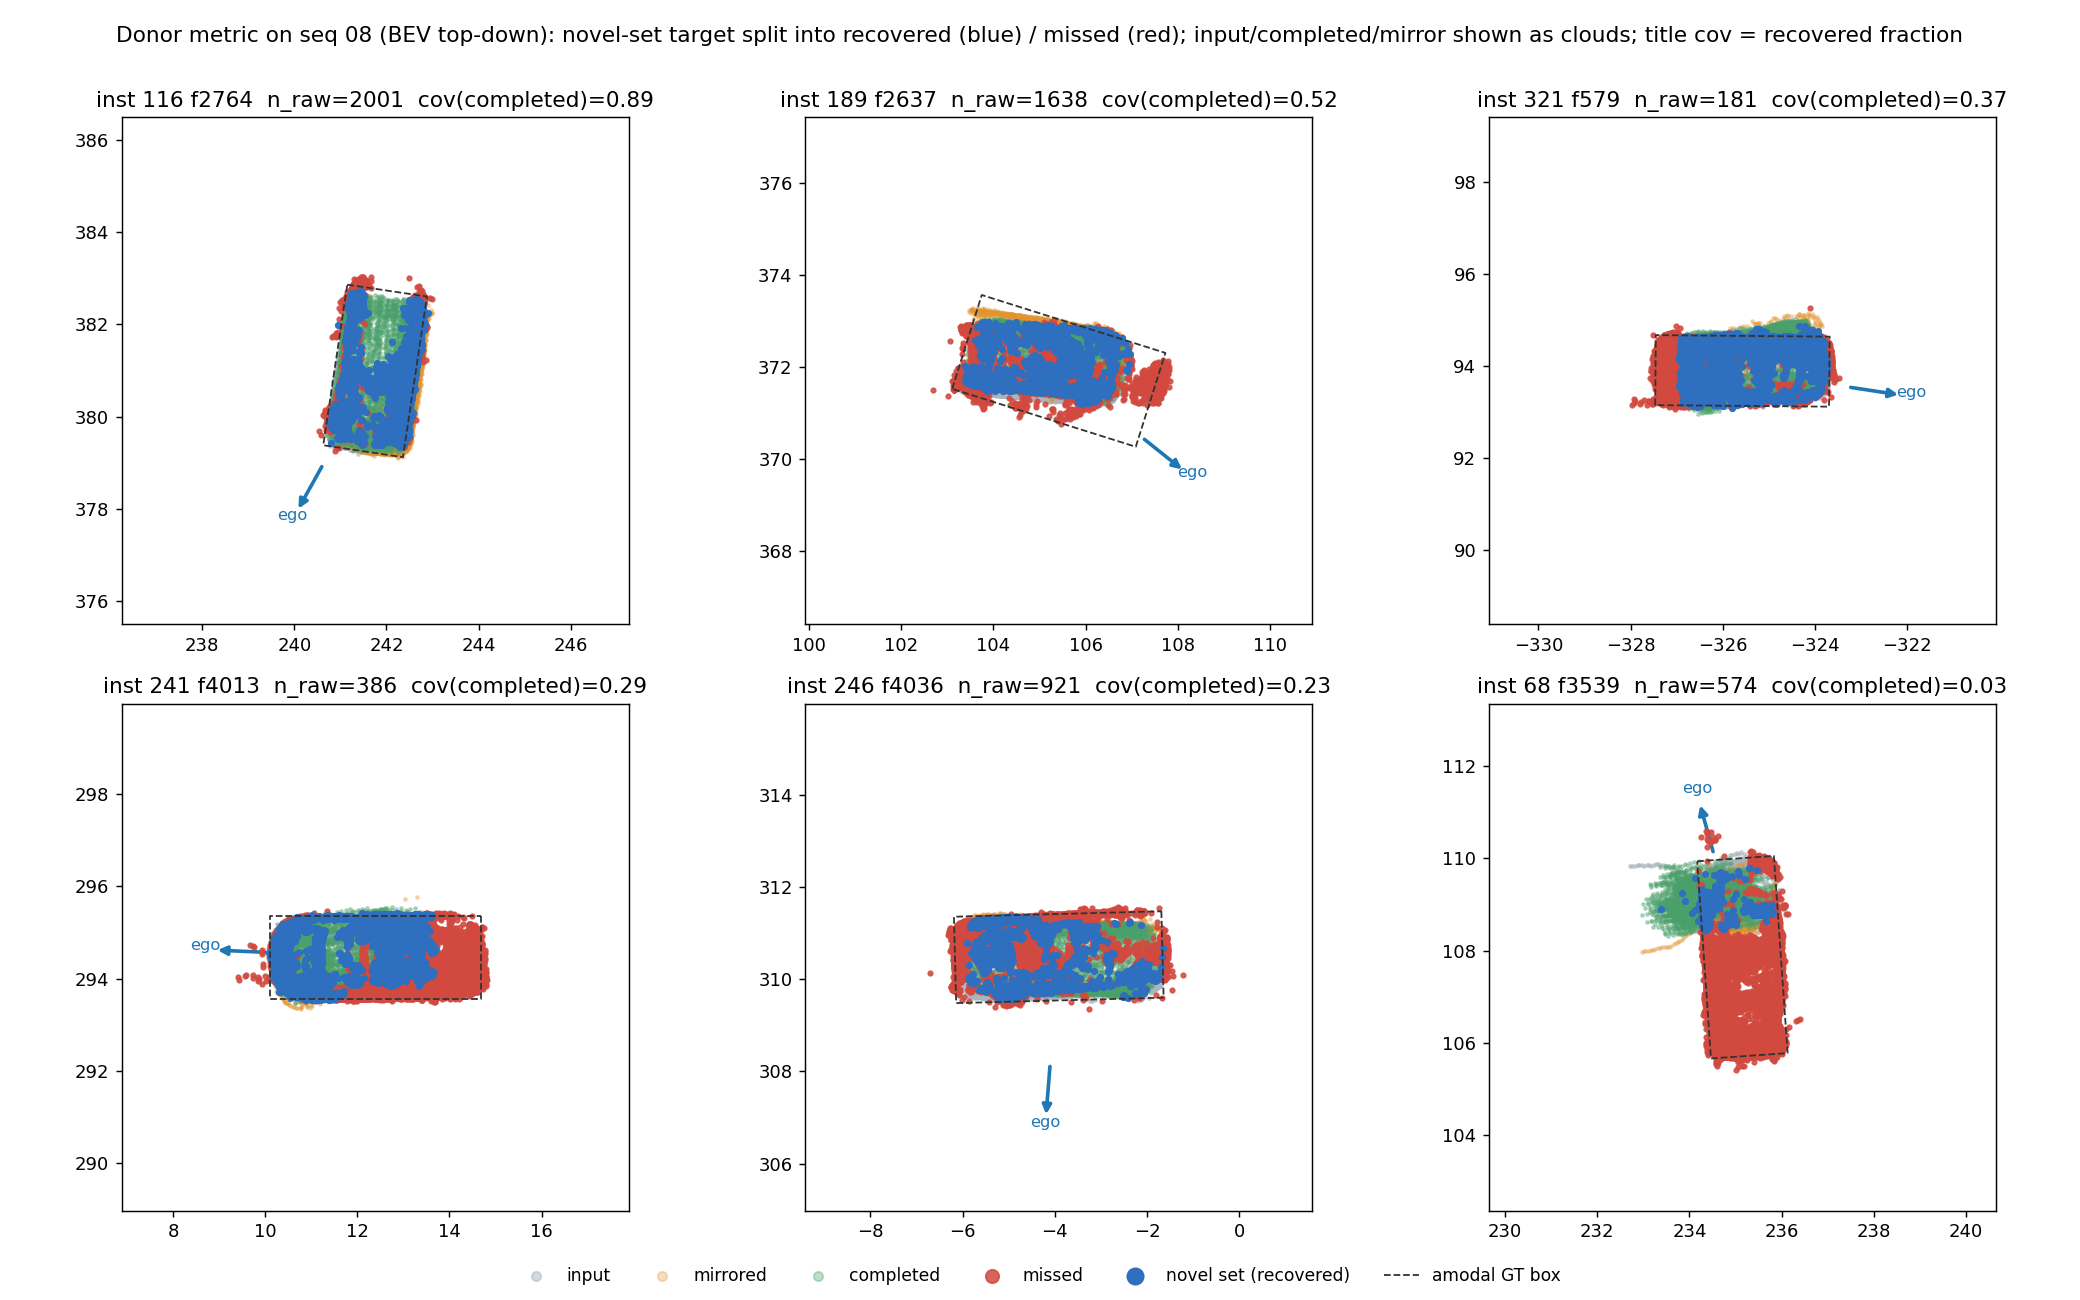
\includegraphics[width=\linewidth]{donor_metric_08.png}
  \caption[The donor metric on six seq-08 cars]{The donor metric in bird's-eye view on six seq-08 cars, spanning the
    coverage range from best (top-left) to a residual failure (bottom-right). The
    \emph{novel set} --- the donor-only surface the input frame never saw --- is
    drawn blue where the completion recovers it within \SI{0.1}{\meter} and red
    where it does not, so the blue fraction of the target is exactly the reported
    \texttt{cov@0.1} in each title. The three candidate clouds are shown faintly
    for context: the input partial (grey), its symmetry mirror (orange), and the
    completion itself (green). The upper panels close the occluded far side almost
    entirely; the last isolates the residual failure modes --- far-end
    under-completion and heading/centre error on diagonal or sparse views --- that
    Section~\ref{sec:results-box} and Section~\ref{ch:completion-method} address.
    Rendered by \texttt{scratchpad/donor\_metric\_viz.py}.}
  \label{fig:donor-coverage}
\end{figure}

\section{Downstream utility: the amodal bounding box}
\label{sec:results-box}

Surface coverage shows the completion is geometrically faithful; the box
evaluation shows it is \emph{useful}. For each true-positive (frame, car) pair on
the well-observed static cars we fit an oriented box to the raw partial and to the
completion with the \emph{same} fitter used to build the amodal ground-truth
boxes (so fitter bias cancels), and compare each against the GT box. This is the
pre-registered ``completion adds value'' test.
Table~\ref{tab:box-quality} reports it.

\begin{table}[H]
  \centering
  \caption[Amodal box quality: raw partial vs.\ completion]{Amodal box quality, raw partial vs.\ completion (seq~08, per-car
    medians, $n=39$ of the \num{40} well-observed static cars --- one has no
    completed pair). BEV IoU is the oriented
    bird's-eye-view box overlap; $|\Delta W|,|\Delta H|,|\Delta L|$ are absolute
    dimension errors; centre error is in the ground plane. $p$ is the Wilcoxon
    signed-rank across cars. These figures use the original detection
    configuration; the width, height, and overlap wins reproduce under the promoted
    configuration of Table~\ref{tab:length-geometry} (BEV IoU
    \num{0.725}$\to$\num{0.747}, $|\Delta W|$ \num{0.210}$\to$\num{0.122},
    $|\Delta H|$ \num{0.227}$\to$\num{0.144}).}
  \label{tab:box-quality}
  \begin{tabular}{lcccl}
    \toprule
    Metric & Raw & Completed & Wilcoxon $p$ & \\
    \midrule
    BEV IoU $\uparrow$        & 0.707 & \textbf{0.747} & \num{1.9e-3}  & better \\
    $|\Delta W|$ (m) $\downarrow$ & 0.270 & \textbf{0.170} & \num{1.5e-4}  & better \\
    $|\Delta H|$ (m) $\downarrow$ & 0.255 & \textbf{0.131} & \num{1.6e-10} & better \\
    centre err.\ (m) $\downarrow$ & 0.286 & \textbf{0.234} & \num{2.8e-5}  & better \\
    $|\Delta L|$ (m) $\downarrow$ & 0.447 & 0.456          & 0.65          & neutral \\
    yaw err.\ (deg) $\downarrow$  & 3.5   & 3.0            & 0.74          & neutral \\
    \bottomrule
  \end{tabular}
\end{table}

Completion improves the box on width, height, centre, and overall BEV overlap
with strong significance, and nothing degrades significantly. The improvements
are largest where the sensor saw least --- BEV IoU by input size rises
\num{0.461}$\to$\num{0.599} on the sparsest cars (${<}100$ points),
\num{0.585}$\to$\num{0.678} at \num{100}--\num{300}, and \num{0.703}$\to$\num{0.744}
above \num{300} --- which is the right profile for the use case, since a
well-observed car needs little help. The width gain is not an artefact of the
GT accumulation: it holds both for the \num{13} cars whose width the accumulation
genuinely constrains (both flanks eventually seen: \num{0.291}$\to$\num{0.182})
and for the other \num{26} (\num{0.167}$\to$\num{0.118}).

\paragraph{Length was the exception, and the geometry work fixed it.} In
Table~\ref{tab:box-quality} length is neutral --- the completion neither helps nor
hurts $|\Delta L|$. That was too generous a reading of an untreated defect: the
completion of a partial truncated at the occluded far end stops short, so it
\emph{under}-completes length. Table~\ref{tab:length-geometry} isolates this on
the promoted configuration ($n=40$) and tracks the two Section~\ref{ch:completion-method} fixes ---
the fixed \SI{4.14}{\meter} prior and the per-car length estimate --- against the raw partial and the completion \emph{without} any
length correction.

\begin{table}[H]
  \centering
  \caption[Length geometry on the amodal box]{Length geometry on the amodal box (seq~08, well-observed static cars,
    per-car medians, $n=40$, promoted configuration).
    ``no prior'' is the completion with the canonical-frame centre but no
    longitudinal push; ``fixed \SI{4.14}{}'' is the population-median prior;
    ``per-car'' is the final \nth{90}-percentile track estimate. The compact
    row is signed $\Delta L$ on cars ${<}\SI{3.6}{\meter}$ ($n=8$), where a fixed
    prior over-extends.}
  \label{tab:length-geometry}
  \begin{tabular}{lcccc}
    \toprule
    Metric & Raw & no prior & fixed \SI{4.14}{} & \textbf{per-car (final)} \\
    \midrule
    $|\Delta L|$ (m) $\downarrow$   & 0.428 & 0.476 & 0.354 & \textbf{0.304} \\
    BEV IoU $\uparrow$              & 0.725 & 0.743 & 0.747 & \textbf{0.771} \\
    centre err.\ (m) $\downarrow$   & 0.271 & 0.227 & 0.229 & \textbf{0.184} \\
    \midrule
    compact signed $\Delta L$ (m)   & $-0.007$ & --- & $+0.295$ & \textbf{$+0.063$} \\
    \bottomrule
  \end{tabular}
\end{table}

Two things are visible here, and both are stated as the honest picture rather
than the flattering one. First, Table~\ref{tab:box-quality}'s neutral
$|\Delta L|$ averages over- and under-completion and so hides a real regression:
the \emph{signed} length shows the completion systematically \emph{under}-extends
the occluded far end (normal cars $-0.485\to-0.545$). On the
promoted configuration this surfaces even in the absolute $|\Delta L|$, where
completion \emph{without} a length prior makes box length \emph{worse} than the
raw partial (\num{0.428}$\to$\num{0.476}, $p=0.027$), which the far-end truncation
causes. The fixed prior
reverses it (\num{0.354}) and the per-car estimate improves it further
(\num{0.304}) while lifting BEV IoU to \num{0.771} and cutting centre error to
\num{0.184}. Second, moving from the fixed prior to the per-car estimate is what
removes the over-extension of genuinely compact cars: their signed $\Delta L$ goes
from \num{+0.295} (the fixed median over-extends a short car) to \num{+0.063}
($p=0.016$ at $n=8$), with the same fix showing up in the per-band hallucination
guard of Section~\ref{sec:donor-metric}.

\paragraph{The trade-off, stated plainly.} The per-car estimate buys this box
accuracy at a measured cost in donor coverage: pooled completed \texttt{cov@0.1}
falls \num{0.403}$\to$\num{0.364} and far-end coverage \num{0.346}$\to$\num{0.316}
relative to the fixed prior. Per band it is better on compact and
long cars and worse on normal ones. The two metrics genuinely disagree here, and
a control run settled which reading is right: deliberately over-extending
(\nth{90} percentile $+\SI{0.45}{\meter}$) improved \emph{both} coverage and the
box on normal and long cars, which means those completions are still honestly too
short rather than the metric being fooled. In other words the per-car estimate
trades a little pooled coverage --- driven by the normal band it slightly
shortens --- for a correctly-sized box across all bands, and the residual
shortfall is a real limitation, addressed next.

\paragraph{A bounded negative on the residual shortfall.} Targeting each car's
\emph{true} length still leaves completions short on normal and long cars, which
pointed to a second under-extension mechanism inside the completion itself (PCN
under-fills its normalised frame, and the centre push doubles as an output
rescale). Section~\ref{ch:completion-method} investigated this under pre-registration (the
``closed negative''): decoupling the scale from the length push and adding a
calibrated fill factor did fix the target (normal-car $|\Delta L|$
\num{0.329}$\to$\num{0.232}) but over-extended compacts and failed the
pre-registered compact non-regression guard on both test sequences. The verdict
was to reject it; the knobs stay in the code defaulted off. It is reported here
because it \emph{bounds} the result: the residual far-end shortfall on long cars
is a characterised, length-dependent limit, not an oversight.

\begin{figure}[htbp]
  \centering
  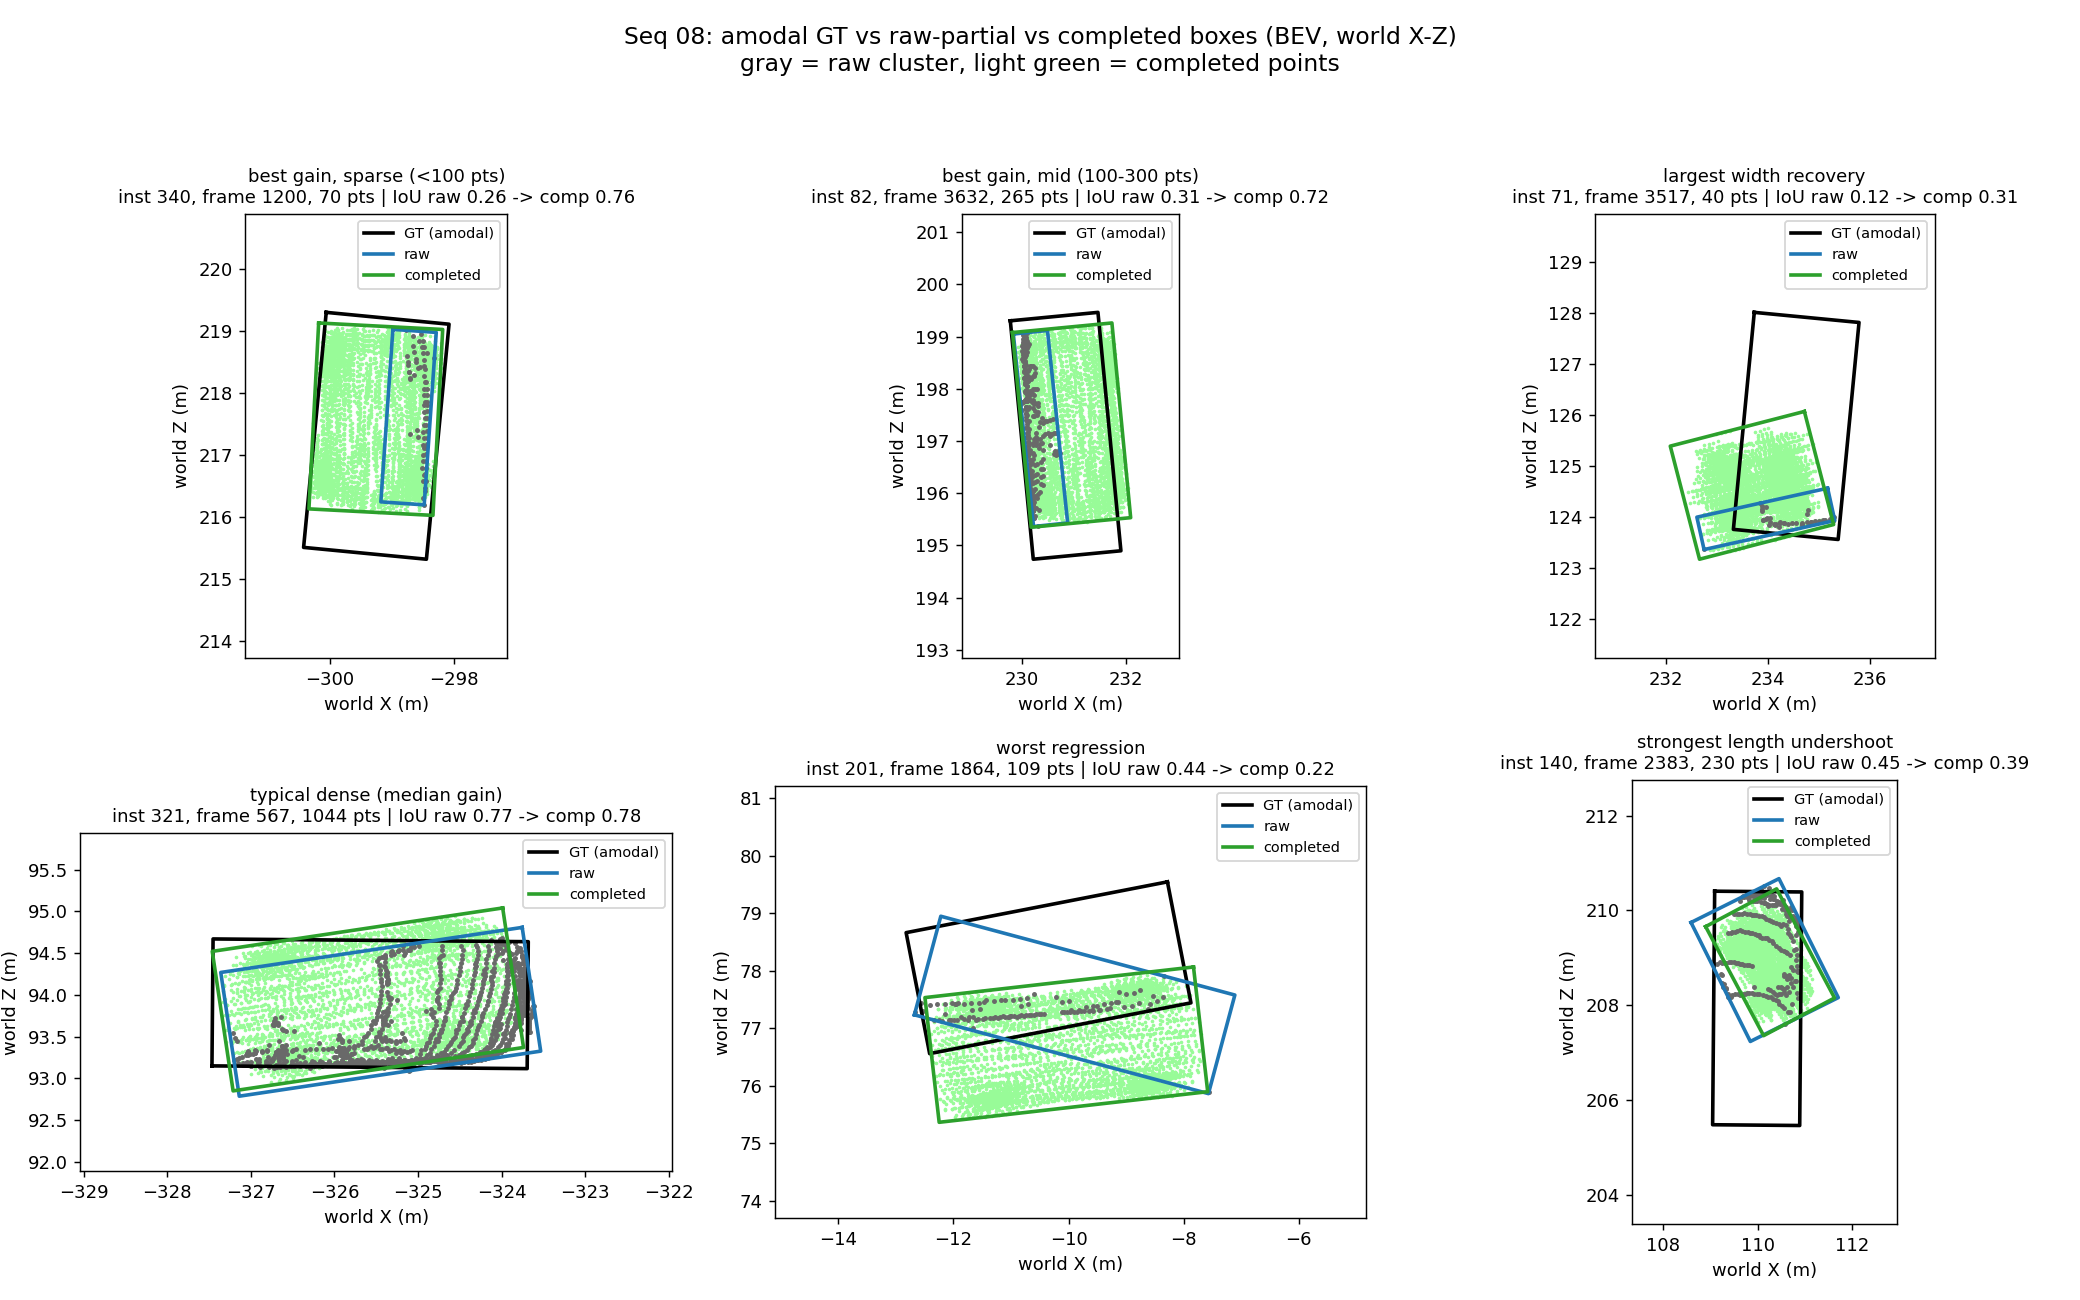
\includegraphics[width=\linewidth]{completion_box_overlays_08.png}
  \caption[Amodal box overlays on six seq-08 cars]{Amodal box overlays on six seq-08 cars: the ground-truth box (black),
    the box fitted to the raw single-frame partial (blue), and the box fitted to
    the completion (green), over the raw points (grey). The completion tightens
    the box on the occluded width and far end and centres it better; the one
    strong regression panel is a heading error on a sparse (\num{109}-point)
    input, a diagonal-view failure mode also visible in
    Figure~\ref{fig:donor-coverage}. Rendered by
    \texttt{scratchpad/completion\_box\_eval\_viz.py}.}
  \label{fig:box-overlays}
\end{figure}

\section{Moving cars}
\label{sec:results-movers}

Both metrics so far are defined on \emph{static} cars by construction: a paired
amodal reference needs a stationary target. Production nonetheless completes
moving cars, and those completions were never validated. Because completion runs
on a single reference frame's cluster --- not on accumulated points --- there is
no motion smear in its input, so there is a mechanistic reason to expect motion
not to matter; this section checks it. On the final seq-08 output
(\num{518} completed car tracks) each track is labelled static, moving, or
ambiguous by the net horizontal displacement of its centroid (a label-free proxy,
since the output tracks are unlabelled), and each completion is scored by a
size-plausibility recipe (bird's-eye dimensions falling in the car range).
Table~\ref{tab:movers} gives the result.

\begin{table}[H]
  \centering
  \caption[Completion plausibility by track motion]{Completion plausibility by track motion (final seq-08 output,
    \num{518} completed car tracks). Motion is the net displacement
    of the track centroid (median of first vs.\ last five frames). Plausible =
    bird's-eye dimensions in the car range ($L\in[3.3,4.9]$, $W\in[1.5,2.1]$,
    $H\in[1.1,1.7]$~m).}
  \label{tab:movers}
  \begin{tabular}{lcccc}
    \toprule
    Group (net displacement) & $n$ & plausible & rate & median $L/W/H$ (m) \\
    \midrule
    static ($\leq\SI{2}{\meter}$)   & 419 & 225 & \SI{53.7}{\percent} & 3.81 / 1.94 / 1.49 \\
    \textbf{moving ($\geq\SI{5}{\meter}$)} & \textbf{19} & \textbf{11} & \textbf{\SI{57.9}{\percent}} & 3.84 / 2.05 / 1.44 \\
    ambiguous (\SIrange{2}{5}{\meter}) & 80  & 46  & \SI{57.5}{\percent} & 3.95 / 1.92 / 1.49 \\
    all                             & 518 & 282 & \SI{54.4}{\percent} & 3.83 / 1.94 / 1.49 \\
    \bottomrule
  \end{tabular}
\end{table}

Moving cars complete \emph{no worse} than static ones --- slightly higher, in
fact (\SI{57.9}{} vs.\ \SI{53.7}{\percent}), well within noise at $n=19$ --- with
near-identical median dimensions, and every motion bucket clusters at
\SIrange{54}{58}{\percent}. Motion does not degrade completion plausibility, as
the single-frame input predicts. One honest caveat about the absolute level, not
the comparison: the plausibility recipe uses axis-aligned dimensions, which
overestimate width and length for cars oriented diagonally to the world axes, so
the \raisebox{0pt}[0pt][0pt]{$\sim$}\SI{54}{\percent} rate \emph{understates}
completion quality (most failures are inflated width on genuine car-shaped
footprints). Since both groups use the identical recipe, the static-vs-moving
conclusion is unaffected. The value of the check is that the statics-only design
of the earlier sections does not hide a mover failure mode.

\begin{figure}[htbp]
  \centering
  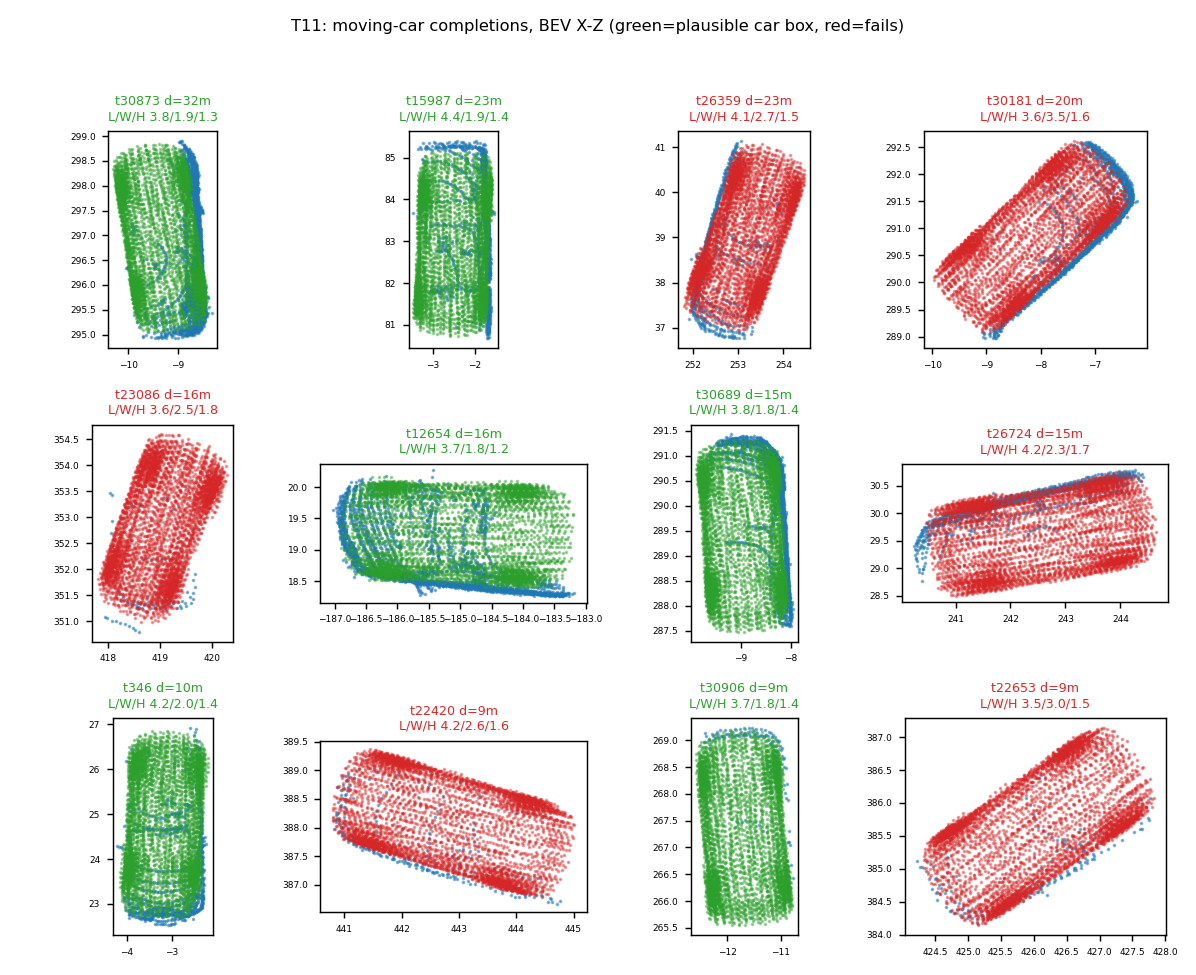
\includegraphics[width=\linewidth]{t11_mover_completions_bev.png}
  \caption[Completions of moving-car tracks on seq~08]{Bird's-eye completions of moving-car tracks on seq~08 (blue partial
    input, green completion). Most form recognisable car footprints; the failures
    are width inflation on diagonally-oriented cars, an artefact of the
    axis-aligned plausibility measure rather than of motion. Rendered by
    \texttt{scratchpad/t11\_mover\_plausibility.py}.}
  \label{fig:movers}
\end{figure}

\section{A pre-registered held-out replication}
\label{sec:results-heldout}

The completion constants --- the width and length priors, the scale correction,
the gate thresholds --- were all developed on seq~08. A fair test of whether the
method \emph{generalises} therefore has to run on a sequence that took no part in
that development, under a protocol fixed in advance so the outcome cannot be
reinterpreted after the fact. We pre-registered one (\texttt{preregistration\_heldout.md},
committed with an immutable timestamp before any held-out run). The held-out
sequence is seq~00 (seq~05 had too few well-observed
static cars to test); the two \emph{primary} metrics were fixed as BEV box IoU
(Section~\ref{sec:results-box}) and donor \texttt{cov@0.1}
(Section~\ref{sec:results-coverage}), each requiring the completion to beat the
raw partial with $p<0.05$; three refutation rules (fails to generalise / seq-08
specific length constants / an uncovered result) and a three-level outcome
taxonomy were registered alongside. Nothing was retuned for seq~00.

One confound is logged rather than hidden: seq~00 is in the classifier's training
split, so its \emph{detection} recall reads optimistically. This does not touch
the completion claim, which is a \emph{paired} raw-vs-completed comparison on
identical true-positive inputs, and PCN was trained only on synthetic data and
never saw seq~00. Table~\ref{tab:heldout} gives the outcome on the \num{45}
well-observed static cars.

\begin{table}[H]
  \centering
  \caption[Held-out replication on seq~00]{Held-out replication on seq~00 (well-observed static cars, per-car
    medians, $n=45$; the two pre-registered primaries in bold, secondary
    dimensions below). Both primaries are decisive wins over the
    raw partial.}
  \label{tab:heldout}
  \begin{tabular}{lccl}
    \toprule
    Metric & Raw & Completed & Wilcoxon $p$ \\
    \midrule
    \textbf{BEV IoU} $\uparrow$          & \textbf{0.739} & \textbf{0.766} & \textbf{\num{1.6e-3}} \\
    \textbf{donor \texttt{cov@0.1}} $\uparrow$ & \textbf{0.000} & \textbf{0.413} & \textbf{${\approx}0$} \\
    $|\Delta W|$ (m) $\downarrow$        & 0.203 & 0.165 & \num{4.0e-4} \\
    $|\Delta H|$ (m) $\downarrow$        & 0.278 & 0.120 & \num{7.8e-9} \\
    \bottomrule
  \end{tabular}
\end{table}

Both headline claims replicate: on a sequence that played no part in tuning, the
completion beats the raw partial on box overlap (\num{0.739}$\to$\num{0.766},
$p=\num{1.6e-3}$) and on surface coverage (\num{0.000}$\to$\num{0.413},
$p\approx0$), with the secondary width and height errors improving as they did on
seq~08. Applying the pre-registered rules verbatim, the arbitration verdict was
\textbf{partially holds}: neither generalisation rule triggered ---
both primaries won and no testable length band regressed against its seq-08 level
--- but seq~00's well-observed set contains \emph{no} long cars
(${\geq}\SI{4.6}{\meter}$), so the long-band predictions and the long-band
hallucination guard are simply untestable on it. The downgrade from ``holds'' to
``partially holds'' is therefore a \emph{coverage gap in the held-out data, not a
weak result}: everything that could be tested passed, and the one thing that could
not be tested is a property of seq~00's car population, not of the method.

\section{Summary and limitations}
\label{sec:results-summary}

The completion method rests on three measured results. It adds genuinely unseen
surface --- about \SI{30}{\percent} of never-observed surface within
\SI{0.1}{\meter}, seven times the symmetry-mirror baseline, with essentially no
hallucination (Section~\ref{sec:results-coverage}). It improves the amodal box on
width, height, centre, and overall overlap, most where the sensor saw least, and
the length-geometry work turns an untreated length regression into a net gain
(Section~\ref{sec:results-box}). And both headline claims survive a
pre-registered replication on a held-out sequence
(Section~\ref{sec:results-heldout}). Moving cars, which the static-car metrics
cannot score, complete no worse than static ones
(Section~\ref{sec:results-movers}).

The limitations are stated as findings, each already quantified. The
\emph{far end} of the car is the weakest-covered region, and on long cars the
residual under-extension is a characterised, length-dependent limit that a
pre-registered fix could not remove without regressing compacts.
The per-car length estimate falls back to the fixed population prior on
\SI{23}{\percent} of final tracks --- those with fewer than five gate-passed
frames --- which is above a comfortable threshold and is not
solved. The sparsest inputs complete more coarsely, and the axis-aligned plausibility
measure inflates the \emph{reported} width of diagonally-oriented cars. And the two quantitative metrics measure static cars directly;
moving cars are covered only by the weaker plausibility check. None of these
overturns the headline --- completion adds unseen surface and a better box, and
generalises --- but they mark exactly where the method is soft, and they set the
agenda for the discussion that follows.
                % Chapter 4: protocol + detection results + recall analysis + donor metric + completion results
% Chapter 5 -- Discussion and Conclusion (\input by main.tex): discussion + limitations
% + RQ answers + contributions + future work (conclusion half merged in below,
% formerly sec_9_conclusion.tex). Synthesises the detection and completion results into
% a single statement of what the thesis supports, then states every audit-identified
% limitation BY NAME so the committee cannot surface one the thesis has not already named.
%
% Honesty-phrasing rules applied (personal_agenda P1):
%   - claims matched to evidence tier (measured / inferred / speculative) explicitly
%   - "mean IoU" always qualified as "of matched detections"
%   - recall denominator restated (>=10 surviving points, Sec 4.1) wherever recall is cited
%   - completion claims scoped per the T9c outcome (PARTIALLY HOLDS) and to static cars
%   - negative results (#40/#45 etc.) presented as findings, not apologised for; #37 as a
%     metric-design lesson
%   - every number traces to a finding / artifact (cited Finding~\#NN)
%   - the six mandatory named limitations are all present: detection selection-exposure
%     (now bounded by LOSO cross-validation, Sec 4.1: precision-only, ~2 pts), statics-only
%     accuracy, compact-band d2, empty long band, 23% length-estimate fallback (#41),
%     SemanticKITTI label-quality assumption -- plus the clustering-objectness ceiling
%     (recall analysis, Ch 4) and the offline-runtime scope
%
\chapter{Conclusion and Future Work}
\label{ch:conclusion}

The preceding chapters reported results; this one interprets them and closes the
thesis. It first draws the conclusions, answering the two research questions and
restating the contributions (Section~\ref{sec:conclusion-rqs}); then gathers what the
evidence supports and how far each claim reaches, together with every limitation the
work carries, into a single section (Section~\ref{sec:disc-limitations}) --- the
validity of the evaluation, the scope of the completion claims, the ground-truth
assumptions, and the architectural and operational limits --- and finally turns the
most consequential boundaries into future work (Section~\ref{sec:conclusion-future}).
Every weakness named here is measured elsewhere in the document and cross-referenced to
the finding that quantifies it: a limitation the thesis names, quantifies, and bounds is
defended; one a committee surfaces first is not.

\section{Conclusion}
\label{sec:conclusion-rqs}

Chapter~\ref{ch:introduction} posed two research questions, both about measuring completion
on real LiDAR; each is answered in full in Section~\ref{sec:donor-validation} and restated
here in the form asked, with its reach discussed in Section~\ref{sec:disc-what-holds}.

\paragraph{RQ1 --- how to evaluate completion on real LiDAR.}
Reference-based Chamfer distance against accumulated pseudo-ground-truth is invalid, because
the accumulated reference is occluded on the same side as the input and so rewards
under-completion; the thesis replaces it with the donor-frame occluded-side coverage metric,
which scores recovery of surface seen only in other frames of the same static car and passes
a four-item validation gate.

\paragraph{RQ2 --- whether completion recovers unseen surface, and whether the benefit holds out.}
Yes, within a named scope. On sequence~08 the donor metric shows PCN recovers genuinely
occluded surface (coverage at \SI{0.1}{\metre} \num{0.000}~$\rightarrow$~\num{0.304} against
the mirror baseline \num{0.043}) and improves the amodal box
(\num{0.725}~$\rightarrow$~\num{0.771}); under a pre-registered test on held-out sequence~00
the benefit \textsc{partially holds} --- both metrics replicate, but the long band was
untestable and the compact guard fails. Moving cars are a plausibility check only.

\paragraph{Diagnostic findings.}
Two findings emerged along the way (Section~\ref{sec:recall-analysis},
Chapter~\ref{ch:evaluation}): recall is clustering-bound, not classifier-bound --- HDBSCAN
splits \SIrange{31}{37}{\percent} of cars and a chain of repair strategies fails to
generalise --- and synthetic pretraining is redundant once real clusters are plentiful, the
sim-to-real gap being total and symmetric.

\paragraph{Contributions.}
The thesis makes a single scientific contribution, methodological rather than architectural:
\textbf{a validated metric for completion quality on real LiDAR}, through which learned
completion is shown to recover genuinely occluded surface and improve amodal boxes on static
cars, partially replicated on a held-out sequence. Two diagnostic findings sit alongside it
--- the clustering-bound recall account and the redundancy of synthetic pretraining --- with
engineering contributions (the modular pipeline and its runtime characterisation, the amodal
box builder, the reproducibility infrastructure) and documented negative-result lines.

\section{Limitations and Discussion}
\label{sec:disc-limitations}

\subsection{Established Results and Their Reach}
\label{sec:disc-what-holds}

Two threads carry the strongest evidence, both belonging to the metric contribution. The
first is methodological: the donor-frame occluded-side coverage metric
(Section~\ref{sec:donor-validation}). We are not aware of a prior metric that scores a real
LiDAR car's completion against donor frames of the same static instance --- the reference-free
measures reviewed in Section~\ref{sec:bg-completion} all score against the observed input, a
synthetic prior, or the model's own outputs, and the closest prior construction (Ren et
al.~\cite{ren2022selfsupervised}) scores the accumulated cloud as a whole, not the
never-observed surface. It also carries a measured negative result about metrics: the obvious
alternative --- Chamfer distance against accumulated pseudo-ground-truth --- is invalid,
because accumulated LiDAR is itself one-sided and rewards under-completion (the raw partial
scored the lowest Chamfer distance on every real example), as do the field's standard
input-referenced UCD/UHD (Section~\ref{sec:reffree-compare}). The second thread is empirical
and rests on that metric: completion adds genuinely unseen surface (median occluded-side
coverage within \SI{0.1}{\metre} of \num{0.304} on sequence~08, against \num{0.043} for the
symmetry mirror and \num{0.000} for the raw partial) and improves the amodal box (median BEV
IoU \num{0.725}~$\rightarrow$~\num{0.771}, gains concentrated where the sensor saw least);
both survive a pre-registered held-out replication with named caveats (\textsc{partially
holds}; Section~\ref{sec:disc-eval-validity}).

The detection pipeline is a strong engineering result rather than a claim of
state-of-the-art accuracy: the supervised networks positioned in
Section~\ref{sec:bg-positioning} reach higher accuracy at the dense annotation cost this
pipeline avoids. It reaches precision \num{0.905}, recall \num{0.730}, $F_1$~\num{0.808} on
the full sequence~08 (mean IoU of matched detections \num{0.912}; recall denominator: car
instances with at least \num{10} points surviving preprocessing,
Section~\ref{sec:eval-protocol}), with an interpretable, near-annotation-free clustering
front end on modest hardware. Its recall shortfall is root-caused, not mysterious --- HDBSCAN
splitting large, close cars into fragments (Section~\ref{sec:recall-analysis}) --- and that
diagnosis, with the finding that synthetic pretraining is redundant at scale, are the two
secondary results the investigation produced.

These reaches vary. The detection operating point is the broadest, cross-validated across
all eleven labelled sequences (Section~\ref{sec:eval-loso}). Two completion results transfer
by argument rather than by sample --- the invalidity of accumulated-Chamfer follows from the
one-sidedness of accumulated LiDAR, and the donor metric is dataset-agnostic wherever static
cars are seen from multiple frames --- whereas the recall diagnosis is an inductive result
from two sequences, mechanistic but not a proven invariant. The tuned constants (the length
prior, the estimate quantile, the geometric thresholds) are sequence-derived and should be
re-checked on a new sensor, and the completion accuracy claims are scoped to static,
gate-passed cars in the compact and normal bands. For practice, three readings follow: the
interpretable, near-annotation-free detector is a viable choice where labelling budget or
inspectability outweighs peak recall, provided the domain is dense-scene; the donor metric is
a reusable instrument for any real-LiDAR completion where static objects recur across frames;
and because input quality, not model choice, governs whether completion is usable, effort is
better spent on segmentation than on swapping architectures. These reaches are bounded by the
limitations set out next.

\subsection{Validity of the Evaluation}
\label{sec:disc-eval-validity}

Detection is cross-validated, and the selection exposure is precision-only. SemanticKITTI
labels only sequences \numrange{00}{10}, so no labelled sequence can be reserved as a
conventional held-out detection test set, and the final classifier was historically selected
on sequence~08; leave-one-sequence-out cross-validation (Section~\ref{sec:eval-loso}) bounds
the exposure, the fold-08 classifier matching its recall (\num{0.737} versus \num{0.730}) and
losing only about two precision points (\num{0.881} versus \num{0.905}), so the selection
touched precision, not the clustering-imposed recall ceiling (\num{0.775}) that accounts for
most missed cars. Completion is held out more strongly still --- its claims are re-tested on
sequence~00 under a pre-registration and the model never saw a real sequence --- and that
replication returned \textsc{partially holds}: both primary metrics were decisive wins (BEV
IoU \num{0.739}~$\rightarrow$~\num{0.766}, $p=\num{1.6e-3}$; donor coverage
\num{0.000}~$\rightarrow$~\num{0.413}), but the long band was empty (no car
$\geq$~\SI{4.6}{\metre} survived the static-car construction), leaving long-car behaviour
untestable off the tuning sequence, and the compact-band guard fails there as on sequence~08.
The completion value is thus replicated once, not across a range of sequences.

\subsection{Scope of the Completion Claims}
\label{sec:disc-completion-scope}

The quantitative completion claims are bounded in what they can score. Both metrics require a
static car by construction, so moving cars cannot be scored by either and are reported only as
a plausibility check, where they reach plausible boxes at essentially the static rate
(\SI{57.9}{\percent} versus \SI{53.7}{\percent}) --- a parity result, not an accuracy claim,
and a conservative one, since the axis-aligned flag penalises the non-axis-aligned cars movers
over-represent. The metric also scores only clean, gate-passed clusters, and whether a car
reaches completion as one is decided upstream by the clustering that caps recall: the
ablations (Section~\ref{sec:abl-completion}) show the L-shape input gate sharply raises
plausible-completion rates on every sequence whereas swapping PCN for PoinTr changes them not
at all, so widening completion's reach is a segmentation problem, not a
completion-architecture one.

Within that scope, three residuals bound accuracy. The per-car length estimate falls back to
the \SI{4.14}{\metre} population prior on tracks with fewer than five gate-passed frames ---
\SI{23.0}{\percent} of sequence-08 tracks --- reintroducing compact overshoot there; the cost
sits inside the headline gain (median BEV IoU \num{0.725}~$\rightarrow$~\num{0.771}, measured
on the same tracks) and falls on the sparsest, most distant cars where the box matters least.
Even with an unbiased estimate the completed cloud stays slightly short at the far end by an
amount that scales with car length, and a pre-registered fix removed this on normal and long
cars but over-extended compacts, so the compensation is irreducibly length-dependent and the
far end remains the weakest-covered region. Both residuals compound the model's synthetic-only
training --- the source of the evaluation's independence but also the synthetic-to-real gap
(Section~\ref{sec:bg-completion}) behind the residual flatness of real completions --- which
shows most sharply on compact cars, where completions spray points outside the box at roughly
\num{100} times the mirrored baseline under the fixed prior and about \num{16} times under the
per-car estimate; no configuration clears the compact bar, so we report the ratios rather than
tune the guard, a band-localised failure the original pooled-median guard was blind to.

\subsection{Ground-Truth and Dataset Assumptions}
\label{sec:disc-gt}

Three assumptions underlie the ground truth. The amodal box is constructed by accumulating a
static car's frames, since no external amodal reference exists (KITTI raw tracklets for the
sequence-08 drive, \texttt{2011\_09\_30\_drive\_0028}, do not exist on the official archive);
it rests on the paired design comparing raw against completed on the \emph{same} box,
viewpoint- and motion-coverage guards, and a sane dimension distribution, so the claim is
robustness to plausible reference error, not an error-free reference. Recall is reported
against eligible cars --- those with at least \num{10} points surviving preprocessing ---
which excludes \SI{25.5}{\percent} of annotated cars too sparse or distant to reach the front
end, so recall against all annotated cars is approximately \num{0.54} against the \num{0.730}
eligible figure (both reported; the two ``$\geq$10-point'' rules are distinct). And all
counts, matches, and the amodal construction assume SemanticKITTI's labels are correct; we did
not audit them, and mislabelled cars would propagate into both the detection metrics and the
ground truth.

\subsection{Architectural and Operational Limits}
\label{sec:disc-architectural}

The remaining limits are architectural or operational. The recall ceiling is architectural,
not a tuning failure (Section~\ref{sec:recall-analysis}): coarsening the cluster voxel to
\SI{0.10}{\metre} recovered part of the loss (\num{0.699}~$\rightarrow$~\num{0.730}) but
coarsening further fuses adjacent cars, and no fixed-radius density clusterer reaches HDBSCAN's
recall at any tested radius, so the ceiling (\num{0.775} before any learned stage, splitting
\SIrange{31}{37}{\percent} of cars) is the measured price of the interpretable,
near-annotation-free design the thesis exists to evaluate, and lifting it means a learned
detector --- a different system. The operational domain is dense scenes: recall falls to
\num{0.336} on the sparse highway sequence~01 against \num{0.761} on dense-urban sequence~00,
mostly because highway cars are distant and recall collapses with range (\num{0.196} beyond
\SI{40}{\metre}) and partly because the front end was tuned on dense data, though the failure
is a conservative miss, not a false alarm (sequence~01 precision \num{0.951}). The system is
offline by design, running at about \SI{623.5}{\milli\second} per frame
(Section~\ref{sec:results-runtime}) with the $\leq\SI{400}{\milli\second}$ target unreachable
through the authorised tiers, and real-time operation is out of scope. Finally, the centroid
tracker feeds the length estimate and drives the \SI{23}{\percent} fallback but is never
scored as a tracker (no MOTA or IDF1), so its contribution to that fallback is unmeasured.

% Conclusion moved to the top of this chapter (Section~\ref{sec:conclusion-rqs}) to
% mirror the gospel's Conclusion-first order; the Established Results discussion is
% folded into Limitations and Discussion above. Honesty-phrasing rules (personal_agenda
% P1) still apply to the moved Conclusion: held-out outcome PARTIALLY HOLDS (#42),
% moving cars = plausibility only (#44), negatives as findings, claims within C1-C11.

\section{Future Work}
\label{sec:conclusion-future}

The limitations above named the boundaries of the present results. Three of them are the natural next
steps, each already scoped by a finding rather than left open.

\paragraph{A real-time variant.} The pipeline runs offline at roughly
\SI{623.5}{\milli\second} per scan (Section~\ref{sec:results-runtime}), dominated by the
classical CPU stages. The direct speed path is an implementation one: the residual
$\sim$\SI{185}{\milli\second} attributed to clustering is the cost of the \emph{Python}
HDBSCAN, not the HDBSCAN \emph{algorithm}, so a native or GPU implementation would attack
that floor without changing what is computed. Swapping in a faster fixed-radius clusterer is
not a free substitution --- the benchmark shows none reaches HDBSCAN's recall at any tested
radius --- so a real-time variant must preserve the HDBSCAN algorithm via a faster
implementation, or replace the front end with a learned detector, rather than trade measured
recall for speed.

\paragraph{Real-data fine-tuning for completion.} The completion model was trained on
synthetic KITTI-like partials only, which is at once the source of the donor metric's
validity and a ceiling on real-data crispness: on the sparsest, most one-sided inputs the
completions stay flat, which traces to the remaining synthetic-to-real
domain gap. Closing it would call for real-data fine-tuning, which is itself a documented
negative-result line in this project; it is a contingency
direction, to be attempted only with the leakage controls that make real-data supervision
safe.

\paragraph{Long-band amodal ground truth on a second held-out sequence.} The held-out
replication (Section~\ref{sec:results-heldout}) partially held in part because the long length band was empty on
sequence~00 --- no car of at least \SI{4.6}{\metre} survived the well-observed-static-car
construction --- so the per-car length estimate's behaviour on long cars could not be tested
off the tuning sequence. Building amodal ground truth for a third sequence with long cars
present would close that single coverage gap and upgrade the long-band claim from a
sequence-08 result to a replicated one. It is deferred here as a bounded data-construction
task, not a change to the method.

\bigskip

None of the thesis's results rests on an additional point of metric improvement: the
methodological contribution is a validated real-data completion metric, and each empirical
claim --- that learned completion adds genuinely unseen surface and improves amodal boxes on
static cars, that recall is clustering-bound, that synthetic pretraining is redundant at
scale --- is defended by explanation and, where the design allowed it, by a pre-registered
test whose outcome was reportable either way. That is the standard the work set for itself,
and the standard on which it asks to be judged.
     % Chapter 5: discussion + limitations + RQ answers + contributions + future work

% --- Bibliography (single, master-owned) ---
\bibliographystyle{IEEEtran}
\bibliography{../../references}

\end{document}
